\documentclass[a4paper,11pt]{report}

\usepackage[utf8]{inputenc}
\usepackage[T1]{fontenc}
\usepackage{lmodern}
\usepackage[french]{babel}
\usepackage{geometry}
\usepackage{graphicx}
\usepackage{float}
\usepackage{amsmath}
\usepackage{booktabs}
\usepackage{array}
\usepackage{tikz}
\usetikzlibrary{arrows.meta,positioning,calc,decorations.pathreplacing}
\usepackage[hidelinks,unicode]{hyperref}
\Urlmuskip=0mu plus 1mu
\newcommand{\figref}[1]{\hyperref[#1]{figure~\ref*{#1}}}

\geometry{margin=2.5cm}
\setlength{\parindent}{0pt}
\setlength{\parskip}{0.75em}
\newcolumntype{L}[1]{>{\raggedright\arraybackslash}p{#1}}
\renewcommand{\bibname}{Bibliographie et webographie}
\setcounter{tocdepth}{2}

\title{Rapport de stage\\\large Détection et estimation 3D d'une balle rapide par caméra événementielle}
\author{Rigon Ajvazi}
\date{Juillet 2026}

\begin{document}

\pagenumbering{gobble}

\begin{titlepage}
  \centering
  
\includegraphics[width=0.42\textwidth]{images/logo_UCA_Long_300dpi.png}\par
  \vspace{1.2cm}
  {\Large UNIVERSITÉ CLERMONT AUVERGNE\par}
  {\large Clermont-Ferrand\par}
  \vspace{0.4cm}
  \rule{0.35\textwidth}{0.4pt}\par
  \vspace{0.4cm}
  {\large École Universitaire de Physique et d'Ingénierie\par}
  \vspace{0.4cm}
  \rule{0.35\textwidth}{0.4pt}\par
  \vspace{1.2cm}
  {\Large\bfseries RAPPORT DE STAGE\par}
  \vspace{0.3cm}
  {\large 1\textsuperscript{ère} année de Master\par}
  {\large Spécialité: Mécatronique\par}
  \vfill
  {\large Rigon Ajvazi\par}
  \vspace{0.9cm}
  {\LARGE\bfseries Détection et estimation 3D d'une balle rapide par caméra événementielle\par}
  \vfill
  \begin{tabular}{L{0.42\textwidth}L{0.45\textwidth}}
    Période de stage & du 1\textsuperscript{er} avril 2026 au 25 juillet 2026 \\
    Organisme d'accueil & Institut Pascal, Université Clermont Auvergne / CNRS \\
    Soutien financier & Bourse CIR ITPS, International Research Centre on Innovative Transportation and Production Systems, I-SITE CAP 20-25 \\
    Tuteurs de stage & Sébastien Lengagne, Céline Teulière, Antonio Claudio de Sousa dos Santos Filho \\
    Tuteur académique & Benoit Thuilot \\
    Date de soutenance & 4 septembre 2026 \\
  \end{tabular}
  \vfill
  {\small Soutien financier\par}
  \vspace{0.25cm}
  \begin{minipage}{0.54\textwidth}
    \centering
    
\includegraphics[width=\linewidth]{images/logos/cir_itps.png}
  \end{minipage}
  \hfill
  \begin{minipage}{0.36\textwidth}
    \centering
    
\includegraphics[width=\linewidth]{images/logos/isite_cap_20_25.png}
  \end{minipage}
  \vfill
  {\large Année universitaire 2025--2026\par}
\end{titlepage}

\clearpage
\pagenumbering{roman}

\chapter*{Remerciements}
\phantomsection
\addcontentsline{toc}{chapter}{Remerciements}

Je tiens tout d'abord à remercier mon tuteur de stage, Sébastien Lengagne, ainsi que Céline Teulière et Antonio Claudio de Sousa dos Santos Filho, pour leur encadrement, leur disponibilité, leur aide et les échanges qui ont orienté mon travail tout au long du stage. Leur accompagnement m'a permis de mieux comprendre les enjeux de la perception robotique rapide et de situer mon travail dans un contexte de recherche appliquée.

Je remercie également mon tuteur académique, Benoit Thuilot, pour le suivi du stage et pour les conseils apportés dans la structuration du travail. Je remercie plus largement les membres de l'Institut Pascal et les personnes avec lesquelles j'ai pu échanger au cours du stage, pour leur accueil.

Enfin, je remercie l'Université Clermont Auvergne et l'Institut Pascal de m'avoir permis de réaliser ce stage dans un cadre associant robotique, vision événementielle et apprentissage par renforcement.

Ce travail a bénéficié du soutien du Centre International de Recherche \emph{Innovative Transportation and Production Systems} (CIR ITPS) de l'I-SITE CAP 20-25, par l'attribution d'une bourse CIR ITPS.

\clearpage

\chapter*{Résumé du sujet de stage}
\phantomsection
\addcontentsline{toc}{chapter}{Résumé du sujet de stage}

Ce rapport présente le travail réalisé pendant un stage effectué du 1\textsuperscript{er} avril 2026 au 25 juillet 2026 à l'Institut Pascal, unité mixte de recherche de l'Université Clermont Auvergne et du CNRS. Le sujet porte sur la détection et l'estimation 3D d'une balle rapide à partir d'une caméra événementielle DVXplorer, dans la perspective d'une tâche robotique d'interception.

L'objectif du stage est de construire une chaîne de perception capable de transformer le flux d'événements produit par la caméra en une position de balle exploitable par un robot. Cette information doit être suffisamment rapide et cohérente pour préparer une interception, tout en tenant compte des contraintes de calibration, de bruit et de mouvement rapide. Le rapport présente le contexte de l'organisme d'accueil, l'environnement de travail, les choix algorithmiques, les étapes de calibration intrinsèque et extrinsèque, la validation en simulation, les essais d'intégration et d'interception sur le robot UR3e réel et les perspectives pour fiabiliser la chaîne.

\textbf{Mots clés:} caméra événementielle, robotique, estimation 3D, détection de balle, ROS 2, Isaac Lab, apprentissage par renforcement.

\clearpage

\tableofcontents
\clearpage
\pagenumbering{arabic}

\chapter{Introduction}

Le sujet du stage s'appuie sur une situation simple à décrire. Une personne lance une balle vers un robot manipulateur, et le robot doit l'attraper avec un filet à papillon fixé à son effecteur. Pour réussir cette interception, le robot doit connaître très vite la position de la balle, puis utiliser cette information pour placer le filet au bon endroit au bon moment.

Le stage a été réalisé à l'Institut Pascal, au sein de l'Université Clermont Auvergne, du 1\textsuperscript{er} avril 2026 au 25 juillet 2026. Il concerne principalement la partie perception de cette chaîne. La balle est observée avec une caméra événementielle DVXplorer, c'est-à-dire un capteur qui ne fournit pas des images complètes à fréquence fixe, mais des événements datés lorsqu'un changement local de luminosité est détecté. Ce fonctionnement est adapté à une balle rapide, car il donne une information temporelle fine et limite la quantité de données à traiter.

Le problème central est donc de transformer un flux d'événements en une position 3D de balle fiable, avec une latence assez faible pour rester utile à la commande du robot. Une erreur de profondeur ou un retard de quelques millisecondes peut déplacer fortement le point d'interception. La perception doit donc être rapide, robuste au bruit, cohérente dans le temps et compatible avec la calibration entre la caméra et le robot.

Les objectifs généraux du projet sont les suivants:
\begin{itemize}
  \item obtenir une position 3D exploitable de la balle à partir d'une caméra événementielle;
  \item conserver une latence faible pour rendre l'information utilisable pendant le mouvement de la balle;
  \item assurer la cohérence entre la perception, la calibration caméra-robot et la commande d'interception;
  \item identifier les limites de la chaîne avant son intégration complète sur le robot réel.
\end{itemize}

Ce rapport commence par présenter l'organisme d'accueil, l'Université Clermont Auvergne et l'Institut Pascal, ainsi que l'axe de recherche et les équipes qui ont accueilli et encadré le stage. Le chapitre suivant décrit le poste occupé et l'étude confiée, puis cadre le travail: cahier des charges retenu pour la tâche d'interception, vue d'ensemble du système à construire, moyens techniques et organisation des tâches dans le temps. La suite est organisée autour de deux grands blocs techniques. Le premier concerne la perception événementielle de la balle, avec le positionnement du sujet par rapport aux travaux existants, la calibration de la caméra, les deux méthodes d'estimation 3D développées et leur comparaison chiffrée contre une vérité terrain. Le second concerne l'intégration robotique, avec la calibration entre la caméra et le robot, l'apprentissage d'une politique d'interception en simulation et les essais réalisés sur le robot réel, jusqu'à l'interception d'une balle. Le rapport se termine par un bilan des réalisations puis un bilan technique et personnel du stage.

\chapter{Présentation de l'organisme d'accueil}

\section{Université Clermont Auvergne}

L'Université Clermont Auvergne (UCA) est un établissement public expérimental d'enseignement supérieur et de recherche. Elle est issue de deux étapes récentes de structuration du site clermontois, la fusion en 2017 de l'université Blaise-Pascal et de l'université d'Auvergne, les deux universités historiques de Clermont-Ferrand, puis l'adoption du statut d'établissement public expérimental. La nouvelle UCA, sous ce statut, est née le 1\textsuperscript{er} janvier 2021 dans le prolongement de cette structuration et de la démarche I-SITE CAP 20-25; elle intègre notamment Clermont Auvergne INP, qui regroupe les écoles d'ingénieurs du site. Elle rassemble des activités de formation, de recherche et d'innovation sur plusieurs sites à Clermont-Ferrand et dans la région Auvergne.

L'UCA indique rassembler environ 36\,000 étudiants, 350 formations et 47 structures de recherche \cite{uca-universite}. Elle s'organise autour de six instituts qui regroupent les composantes de formation et de recherche par grands domaines. Cette organisation permet de faire le lien entre enseignement supérieur, laboratoires, plateformes expérimentales et partenaires socio-économiques. Le tableau~\ref{tab:identite-organisme} rassemble les principales caractéristiques administratives de l'établissement et de l'unité qui m'a accueilli; les rubriques financières habituelles d'une entreprise, comme le capital social ou le chiffre d'affaires, n'ont pas d'équivalent pour un établissement public et sont signalées comme non applicables plutôt que renseignées par une valeur approximative.

\begin{table}[H]
  \centering
  \caption{Carte d'identité synthétique de l'Université Clermont Auvergne et de l'organisme d'accueil.}
  \label{tab:identite-organisme}
  \begin{tabular}{L{0.31\textwidth}L{0.60\textwidth}}
    \toprule
    Élément & Information \\
    \midrule
    Nom de l'établissement & Université Clermont Auvergne (UCA) \\
    Statut & Établissement public expérimental à caractère scientifique, culturel et professionnel \\
    Adresse du siège & 49 boulevard François-Mitterrand, CS 60032, 63001 Clermont-Ferrand Cedex 1 \\
    Téléphone & 04 73 17 79 79 \\
    SIRET du siège & 130 028 061 00013 \\
    Organisme d'accueil du stage & Institut Pascal, UMR 6602 UCA/CNRS \\
    Adresse de l'Institut Pascal & Campus universitaire des Cézeaux, 4 avenue Blaise Pascal, TSA/CS 60026, 63178 Aubière Cedex \\
    Effectif de l'Institut Pascal & Environ 400 personnes \\
    Activité principale & Formation, recherche et innovation, en particulier en sciences de l'ingénierie pour l'Institut Pascal \\
    Capital social & Non applicable pour un établissement public \\
    \bottomrule
  \end{tabular}
\end{table}

\section{Institut Pascal}

L'Institut Pascal est l'unité de recherche dans laquelle le stage s'est déroulé. Il s'agit d'une unité mixte de recherche et de formation interdisciplinaire, UMR 6602, placée sous la tutelle de l'Université Clermont Auvergne et du CNRS, avec le CHU de Clermont-Ferrand comme tutelle secondaire. L'institut est également membre de Clermont Auvergne INP. Il couvre les sciences de l'ingénierie du site clermontois, qu'il s'agisse du génie des procédés, de la mécanique, de la robotique, de la physique des sciences de l'information ou de l'ingénierie de la santé.

L'Institut Pascal a été créé le 1\textsuperscript{er} janvier 2012 par le regroupement de laboratoires du site clermontois, dont le LASMEA pour l'électronique, l'automatique et la vision, le LaMI pour la mécanique et les ingénieries et le LGCB pour le génie chimique et biochimique, avec l'objectif de rassembler des compétences complémentaires en sciences de l'ingénierie et de favoriser des projets interdisciplinaires \cite{institut-pascal}. Ce périmètre s'est ensuite élargi par fusions successives, en 2017 puis en 2021, jusqu'à couvrir l'essentiel des sciences de l'ingénierie et des systèmes du site. L'institut rassemble environ 400 personnes, dont près de 150 enseignants-chercheurs et chercheurs et presque autant de doctorants \cite{institut-pascal}, et se positionne sur des recherches allant du développement de connaissances fondamentales jusqu'à leur intégration dans des systèmes. Ses domaines d'application principaux sont la mobilité et les transports, l'usine et l'industrie 4.0, ainsi que l'hôpital du futur. Cette orientation explique la place importante donnée aux systèmes robotiques, à la perception, à la commande et aux plateformes expérimentales.

\section{Implantation géographique}
\label{sec:implantation}

L'UCA est un établissement multi-sites. Son implantation dépasse largement Clermont-Ferrand. Outre les campus clermontois, elle est présente à Vichy, Montluçon et Moulins dans l'Allier, à Aurillac dans le Cantal et au Puy-en-Velay en Haute-Loire \cite{uca-universite}. Cette dispersion correspond à une mission d'aménagement du territoire, celle de maintenir une offre de formation supérieure dans des villes moyennes éloignées de la métropole régionale. Les activités de recherche, en revanche, restent très majoritairement concentrées sur l'agglomération clermontoise, où se trouvent les laboratoires et les plateformes expérimentales.

À l'échelle de Clermont-Ferrand, l'université se répartit sur trois ensembles principaux. Le centre-ville accueille le siège de l'établissement et les composantes de droit, d'économie, de gestion et de lettres. Le site santé, proche du CHU, regroupe la médecine et la pharmacie. Enfin, le campus universitaire des Cézeaux, situé à Aubière, à quelques kilomètres au sud-est du centre-ville, rassemble les sciences et technologies, avec les unités de formation en sciences, les écoles d'ingénieurs de Clermont Auvergne INP et les laboratoires associés.

C'est sur le campus des Cézeaux que s'est déroulé mon stage, l'Institut Pascal y ayant son adresse principale. Le laboratoire, la salle accueillant le UR3e et la caméra événementielle, les moyens de calcul et l'atelier d'impression 3D utilisé pour les supports mécaniques se trouvent sur ce même site. L'environnement de travail est décrit plus loin, dans la présentation de l'unité d'accueil (section~\ref{sec:unite-accueil}).

\section{Activités et axes de recherche}

Les activités de l'Institut Pascal concernent principalement la recherche académique, les projets collaboratifs, les contrats avec des partenaires industriels, la participation à des réseaux scientifiques et l'appui à la formation par la recherche.

Ces activités s'appuient sur cinq axes de recherche:
\begin{itemize}
  \item Génie des Procédés, Énergétique et Biosystèmes (GePEB);
  \item Image, Systèmes de Perception, Robotique (ISPR);
  \item Mécanique, Génie Mécanique, Génie Civil, Génie Industriel (M3G);
  \item Photonique, Ondes, Nanomatériaux (PHOTON);
  \item Thérapies Guidées par l'Image (TGI).
\end{itemize}

Ces activités se déclinent dans trois grands domaines d'application. Le premier concerne la mobilité et les transports des biens et des personnes, avec des systèmes plus sûrs, plus autonomes ou plus efficaces s'appuyant sur la mécanique, la robotique, la perception et la modélisation. Le deuxième concerne l'usine et l'industrie 4.0, avec des problématiques de production, d'automatisation, de robotique collaborative, de contrôle et d'interaction humain-machine. Le troisième concerne l'hôpital du futur, dans lequel l'image, les systèmes guidés et les dispositifs d'assistance jouent un rôle important.

L'Institut Pascal participe également à des dispositifs de partenariat structurants, associés à des projets soutenus par l'ANR, l'Union Européenne, la Région Auvergne-Rhône-Alpes ou le programme CAP 20-25, ainsi qu'à des collaborations industrielles comme FactoLab, laboratoire commun lié à Michelin. Cette proximité avec des problématiques réelles explique que les travaux de recherche ne se limitent pas à des modèles théoriques, mais cherchent souvent à produire des solutions testables sur des plateformes expérimentales.

\section{Centre International de Recherche CIR ITPS}

Le Centre International de Recherche \emph{Innovative Transportation and Production Systems} (CIR ITPS) est l'un des dispositifs de l'I-SITE CAP 20-25. Il a pour rôle de fédérer les activités de recherche du site clermontois autour des systèmes innovants pour les transports et la production, de renforcer la visibilité internationale du site et de contribuer au déploiement territorial des activités scientifiques et de valorisation \cite{cir-itps}.

Ses thématiques couvrent plusieurs enjeux liés à la mobilité, à la production et aux systèmes autonomes, de l'autonomie des robots mobiles et des véhicules au développement de cobots mobiles, à la planification des systèmes de production ou de transport, aux nouveaux vecteurs énergétiques et à l'acceptabilité des nouvelles technologies \cite{cir-itps}. Le CIR ITPS rassemble ainsi des compétences qui vont de la mécanique et de la robotique jusqu'à l'aide à la décision, aux matériaux durables et aux sciences humaines.

Le sujet de ce stage s'inscrit principalement dans la partie robotique et perception de ce cadre. L'objectif final, qui consiste à permettre à un robot d'intercepter une balle rapide, correspond à une problématique de système dynamique où la perception, la commande et l'expérimentation doivent être étudiées ensemble. La caméra événementielle répond au besoin d'une perception rapide, tandis que la partie robotique prépare l'utilisation de cette information pour une action physique.

Le stage présenté dans ce rapport a bénéficié d'une bourse CIR ITPS. Cette aide rattache le travail à un cadre de recherche appliquée où les méthodes développées doivent pouvoir être testées sur des systèmes réels ou proches du réel. La mention de ce soutien et l'utilisation des logos CIR ITPS et I-SITE CAP 20-25 répondent aux consignes officielles applicables aux rapports de stage soutenus par ce centre \cite{cir-itps-useful}.

\section{Organisation interne}

La structure interne de l'Institut Pascal repose sur des axes scientifiques qui correspondent à de grands ensembles de compétences. Cette organisation permet de regrouper les chercheurs et personnels techniques par disciplines, tout en favorisant des projets transversaux. Dans le cas de mon stage, la perception événementielle mobilise des notions complémentaires de géométrie 3D, de traitement du signal, de programmation temps réel, de robotique et d'apprentissage. Le sujet se rattache à l'axe ISPR, présenté en détail dans la section suivante avec les deux équipes qui ont encadré le travail. La \figref{fig:organigramme-ip-stage} donne une lecture simplifiée de cette organisation et de la place du stage.

\begin{figure}[H]
  \centering
  \begin{tikzpicture}[
      orgbig/.style={draw, rounded corners=2pt, align=center, text width=0.36\textwidth, minimum height=0.85cm},
      orgsmall/.style={draw, rounded corners=2pt, align=center, text width=0.13\textwidth, minimum height=0.75cm, font=\small},
      orgteam/.style={draw, rounded corners=2pt, align=center, text width=0.22\textwidth, minimum height=0.85cm, font=\small},
      arrow/.style={-{Latex[length=2.5mm]}, thick}
    ]
    \node[orgbig] (tutelles) {Tutelles\\UCA / CNRS};
    \node[orgbig, below=0.8cm of tutelles] (ip) {Institut Pascal\\UMR 6602};
    \node[orgsmall, below=1.0cm of ip, xshift=-5.6cm] (gepeb) {GePEB};
    \node[orgsmall, below=1.0cm of ip, xshift=-2.8cm] (ispr) {ISPR};
    \node[orgsmall, below=1.0cm of ip] (m3g) {M3G};
    \node[orgsmall, below=1.0cm of ip, xshift=2.8cm] (photon) {PHOTON};
    \node[orgsmall, below=1.0cm of ip, xshift=5.6cm] (tgi) {TGI};
    \node[orgteam, below left=0.9cm and 0.35cm of ispr] (maccs) {Équipe MACCS\\robotique et commande};
    \node[orgteam, below right=0.9cm and 0.35cm of ispr] (comsee) {Équipe ComSee\\vision artificielle};
    \draw[arrow] (tutelles) -- (ip);
    \foreach \x in {gepeb,ispr,m3g,photon,tgi} {
      \draw[arrow] (ip.south) -- (\x.north);
    }
    \draw[arrow] (ispr) -- (maccs);
    \draw[arrow] (ispr) -- (comsee);
  \end{tikzpicture}
  \caption{Organigramme simplifié situant le stage dans l'organisation scientifique de l'Institut Pascal.}
  \label{fig:organigramme-ip-stage}
\end{figure}

\section{Unité d'accueil: l'axe ISPR et les équipes MACCS et ComSee}
\label{sec:unite-accueil}

\subsection{L'axe ISPR}

Le stage s'est déroulé au sein de l'axe Image, Systèmes de Perception, Robotique (ISPR), l'un des cinq axes de recherche présentés plus haut. Cet axe travaille dans le domaine de la perception et de la vision artificielle pour la commande de systèmes robotiques. Son objectif scientifique est de développer des concepts théoriques, méthodologiques et architecturaux permettant à un système de percevoir son environnement, d'en extraire une information fiable, puis d'utiliser cette information pour agir \cite{ispr-axe}. Le sujet du stage, transformer le flux d'une caméra événementielle en une position de balle exploitable pour une interception robotique, est une déclinaison directe de cette question.

L'axe regroupe des enseignants-chercheurs, des chercheurs, des ingénieurs et des doctorants, et il est organisé en quatre thèmes complémentaires \cite{ispr-axe}:

\begin{itemize}
  \item ComSee (\emph{Computers that See}), consacré à la vision par ordinateur;
  \item DREAM, consacré aux architectures embarquées et aux systèmes multi-capteurs;
  \item MACCS (Modélisation, Autonomie et Contrôle dans les Systèmes Complexes), consacré à la modélisation et à la commande des systèmes robotiques;
  \item PerSyst, consacré aux systèmes de perception.
\end{itemize}

Ces thèmes partagent des applications communes autour des véhicules et robots mobiles autonomes, de la robotique de manipulation, de la perception embarquée et de l'interaction avec l'environnement. Ils s'appuient sur les plateformes expérimentales du site clermontois et s'inscrivent dans les programmes structurants de l'institut et du CIR ITPS évoqués précédemment, pour lesquels la robotique autonome est une thématique fédératrice.

\subsection{Les équipes MACCS et ComSee}

Au sein de l'axe ISPR, le stage a été co-encadré par des chercheurs de deux équipes dont les compétences correspondent aux deux volets du sujet.

L'équipe MACCS s'intéresse principalement à la modélisation et à la commande de robots mobiles et de manipulateurs, à la vision robotique, à l'asservissement visuel et aux comportements anticipatifs \cite{ip-maccs}. C'est la composante robotique du stage. Le choix du robot UR3e, la définition de la tâche d'interception, l'apprentissage de la politique de commande et les contraintes de sécurité des essais réels relèvent de cette culture scientifique. Mon tuteur principal, Sébastien Lengagne, appartient à cette équipe, de même qu'Antonio Claudio de Sousa dos Santos Filho, doctorant de l'équipe qui a participé à mon encadrement et dont les travaux servent de point de départ à mon stage. Mon tuteur académique, Benoit Thuilot, en est également membre; ses travaux portent sur la commande et la robotique mobile \cite{ip-maccs}.

L'équipe ComSee est consacrée à la vision par ordinateur \cite{ip-comsee}. Ses travaux portent notamment sur la calibration de capteurs et la reconstruction 3D sans contact, la reconnaissance et le suivi temps réel de motifs visuels, y compris par apprentissage, et la localisation de véhicules mobiles. La partie perception du stage, détection de la balle dans le flux événementiel, estimation 3D et calibration de la caméra, s'inscrit directement dans cette thématique, encadrée par Céline Teulière.

Ces travaux de thèse \cite{antonio-stage} portaient sur la vision, l'apprentissage par renforcement et le transfert de compétences pour une tâche robotique dynamique. Ils m'ont assuré une continuité concrète, avec un objectif applicatif déjà défini, un robot disponible et de premières analyses sur lesquelles m'appuyer.

\subsection{Environnement humain et technique du stage}

Au quotidien, le stage s'est déroulé sur le campus des Cézeaux, dans l'environnement d'expérimentation robotique de l'équipe, où sont installés le robot UR3e et la caméra événementielle DVXplorer utilisés pour les essais réels. L'environnement matériel mis à disposition comprend le bras manipulateur et son contrôleur, la caméra événementielle, un poste de travail pour le développement et le traitement temps réel, une station de calcul équipée d'un processeur graphique pour la simulation et l'apprentissage par renforcement, ainsi qu'un accès à l'impression 3D pour la fabrication des pièces mécaniques du projet, comme le support de mire et le support du filet décrits dans la suite du rapport.

L'environnement humain est celui d'une équipe de recherche, où enseignants-chercheurs, doctorants et stagiaires partagent les mêmes espaces, ce qui facilite les échanges informels et l'entraide technique. Le suivi du stage s'est fait par des points réguliers avec les encadrants, au cours desquels les résultats intermédiaires étaient discutés et les orientations suivantes décidées. Cette double appartenance, commande côté MACCS et vision côté ComSee, s'est révélée particulièrement adaptée au sujet, qui exige en permanence de raisonner sur les deux bouts de la chaîne à la fois.

Enfin, l'unité n'est pas isolée dans l'institut. Les questions mécaniques du projet, comme la conception des supports imprimés en 3D ou la rigidité du montage de calibration, touchent aux compétences de l'axe M3G, et l'institut anime des programmes transversaux qui relient les axes entre eux autour des machines et robots intelligents \cite{institut-pascal}.

\subsection*{Positionnement du sujet dans l'organisme}

Le sujet de stage se situe au croisement de plusieurs objectifs de l'Institut Pascal, développer des méthodes de perception, les tester sur des systèmes rapides et préparer leur utilisation dans un contexte robotique. Il ne s'agit pas uniquement de détecter une balle dans une image. Il faut produire une estimation 3D robuste, temporellement cohérente, suffisamment rapide et compatible avec une commande robotique. Le sujet est ainsi représentatif d'une problématique de mécatronique, puisque le résultat dépend à la fois du capteur, de l'algorithme, du modèle géométrique, du logiciel temps réel et du système robotique.

\chapter{Poste occupé, cahier des charges et organisation du stage}
\label{chap:poste-cadrage}

Ce chapitre décrit la fonction que j'ai occupée pendant le stage et l'étude qui
m'a été confiée, puis le cadrage du travail: les exigences retenues pour la
tâche d'interception, la vue d'ensemble du système à construire, les moyens
techniques mis à disposition et le découpage des tâches dans le temps. Les deux
chapitres suivants entrent ensuite dans le détail des deux volets techniques, la
perception événementielle de la balle puis l'intégration robotique.

\section{Poste occupé et étude confiée}

Pendant le stage, j'ai occupé une fonction de développement et d'expérimentation autour d'une chaîne de perception robotique. Le travail confié consistait à étudier comment détecter une balle rapide dans un flux événementiel, estimer sa position 3D, analyser les limites des méthodes mises en place et préparer l'utilisation de cette information par une partie robotique.

La tâche finale à réaliser est de permettre à un robot à 6 degrés de liberté, ici un UR3e, d'attraper une balle lancée vers lui. Pour détecter la balle avec une latence suffisamment faible, le système s'appuie sur une caméra événementielle, dont les données doivent être transformées en une information de position exploitable par le robot.

Les tâches principales ont été les suivantes:
\begin{itemize}
  \item comprendre le fonctionnement de la caméra événementielle et le format des données produites;
  \item développer une chaîne C++/ROS 2 \cite{ros2-docs} de filtrage, regroupement et estimation de la balle;
  \item comparer une méthode par ajustement de cercle avec une méthode par analyse de trace;
  \item utiliser des séquences simulées pour disposer d'une vérité terrain et analyser les erreurs;
  \item identifier les besoins de calibration entre la caméra et le robot;
  \item préparer le lien avec une politique d'interception apprise en simulation.
\end{itemize}

Le tableau~\ref{tab:bilan-realisations}, en conclusion du rapport, récapitule par thème l'ensemble des réalisations techniques produites pendant le stage et l'état atteint pour chacune.

\section{Cahier des charges}
\label{sec:cahier-des-charges}

La tâche visée consiste à attraper au filet une balle lancée à la main vers un
UR3e. Le tableau~\ref{tab:cahier-des-charges} rassemble les fonctions attendues
et les objectifs utilisés pour évaluer la solution.

\begin{table}[H]
  \centering
  \caption{Cahier des charges synthétique du système.}
  \label{tab:cahier-des-charges}
  \small
  \begin{tabular}{L{0.07\textwidth}L{0.83\textwidth}}
    \toprule
    & Exigence \\
    \midrule
    F1 & Estimer la position 3D de la balle à partir du flux d'événements d'une caméra unique. \\
    F2 & Exprimer cette position dans le repère de la base du robot. \\
    F3 & Produire l'estimation à la cadence de la boucle de commande, soit \(60~\text{Hz}\). \\
    F4 & Commander le robot afin d'amener le filet sur la trajectoire de la balle. \\
    F5 & Garder l'émission de commande désarmée par défaut et interruptible à tout instant. \\
    \midrule
    P1 & Obtenir une erreur de position 3D inférieure au rayon utile du filet dans la zone d'interception. \\
    P2 & Conserver des estimations sur une fraction majoritaire du vol observé. \\
    P3 & Garder un temps de calcul très inférieur à la période de boucle de \(16{,}7~\text{ms}\). \\
    P4 & Obtenir une calibration caméra-robot suffisamment précise pour ne pas dégrader sensiblement la position de la balle. \\
    \bottomrule
  \end{tabular}
\end{table}

P1 à P3 sont évaluées contre une vérité terrain simulée à la
section~\ref{sec:comparaison-quantitative}. La calibration correspondant à P4
et les mécanismes de sécurité associés à F5 sont présentés au
chapitre~\ref{chap:robotique}.


\section{Vue d'ensemble du système}
\label{sec:vue-ensemble}


La chaîne de traitement transforme le flux brut d'événements en une position 3D exploitable par la partie robotique. Les événements proviennent soit de la caméra DVXplorer \cite{inivation-dvxplorer}, soit de séquences enregistrées pour répéter les essais. Ils sont d'abord filtrés, corrigés avec la calibration de la caméra, conservés dans une fenêtre temporelle courte puis échantillonnés afin de limiter la charge de calcul. Les points restants sont ensuite regroupés spatialement pour isoler la balle, puis analysés par une méthode d'estimation 2D, par cercle ou par trace. Cette estimation est convertie en position 3D, visualisée dans l'interface et publiée dans ROS 2 \cite{ros2-docs}. La position est ensuite envoyée à l'agent PPO, qui calcule les actions à appliquer au robot pour placer le filet d'interception. La \figref{fig:chaine-traitement} résume cet enchaînement et sert de fil conducteur au reste du rapport, dont les deux chapitres suivants détaillent chacun de ces blocs, de la calibration de la caméra jusqu'à la commande du robot.

\begin{figure}[H]
  \centering
  \resizebox{\textwidth}{!}{%
  \begin{tikzpicture}[
      font=\small,
      block/.style={draw, rounded corners=2pt, align=center, text width=2.25cm, minimum height=1.05cm},
      source/.style={block, fill=blue!8},
      prep/.style={block, fill=cyan!8},
      estimate/.style={block, fill=orange!12},
      output/.style={block, fill=green!10},
      control/.style={block, fill=purple!10},
      robot/.style={block, fill=red!8},
      arrow/.style={-{Latex[length=2.5mm]}, thick}
    ]
    \node[source] (input) at (0,0) {DVXplorer\\ou replay};
    \node[prep] (preprocess) at (2.65,0) {Prétraitement\\filtrage, correction};
    \node[prep] (cluster) at (5.3,0) {Cluster balle\\fenêtre d'événements};
    \node[estimate] (estimate2d) at (7.95,0) {Estimation 2D\\cercle ou trace};
    \node[output] (pose3d) at (10.6,0) {Position 3D\\repère caméra};
    \node[output] (ros) at (13.25,0) {Publication ROS 2\\position balle};
    \node[control] (ppo) at (15.9,0) {Agent PPO\\calcule l'action};
    \node[robot] (robot) at (18.55,0) {UR3e + filet\\exécute l'action};

    \draw[arrow] (input) -- (preprocess);
    \draw[arrow] (preprocess) -- (cluster);
    \draw[arrow] (cluster) -- (estimate2d);
    \draw[arrow] (estimate2d) -- (pose3d);
    \draw[arrow] (pose3d) -- (ros);
    \draw[arrow] (ros) -- (ppo);
    \draw[arrow] (ppo) -- (robot);

    \node[align=center, font=\footnotesize, text width=14.5cm] at (9.25,-1.55)
      {Principe: ne pas reconstruire une image complète, mais garder les événements utiles pour produire rapidement une position de balle exploitable par la commande robotique.};
  \end{tikzpicture}}
  \caption{Vue simplifiée de la chaîne de traitement C++/ROS 2 \cite{ros2-docs}, depuis l'estimation 3D de la balle jusqu'à l'action calculée par l'agent PPO.}
  \label{fig:chaine-traitement}
\end{figure}

\section{Moyens techniques}
\label{sec:moyens-techniques}


L'environnement technique du stage combine plusieurs outils matériels et logiciels. La caméra DVXplorer \cite{inivation-dvxplorer} fournit les événements utilisés par les méthodes de détection. Les données peuvent provenir de la caméra réelle ou de séquences enregistrées, ce qui permet de répéter les essais et de comparer plusieurs versions de l'algorithme dans les mêmes conditions. Le traitement est réalisé principalement en C++, car la tâche impose une vitesse de calcul élevée et une latence faible, l'information produite devant rester utilisable pour une interception rapide. ROS 2 \cite{ros2-docs} est utilisé pour publier les résultats et préparer l'intégration avec la chaîne robotique. Une interface adaptée au projet est également développée avec raylib \cite{raylib}, une bibliothèque C/C++ légère destinée aux affichages graphiques interactifs, afin de visualiser les événements, les détections et les estimations 3D pendant les essais. Le tableau~\ref{tab:moyens-techniques} récapitule ces moyens et l'usage qui en est fait.

\begin{table}[H]
  \centering
  \caption{Principaux moyens techniques mobilisés pendant le stage.}
  \label{tab:moyens-techniques}
  \begin{tabular}{L{0.28\textwidth}L{0.62\textwidth}}
    \toprule
    Élément & Utilisation dans le stage \\
    \midrule
    Caméra événementielle DVXplorer \cite{inivation-dvxplorer} & Acquisition d'événements à faible latence pour suivre une balle rapide. \\
    Séquences enregistrées & Relecture des essais pour tester les algorithmes de manière reproductible. \\
    C++ et ROS 2 \cite{ros2-docs} & Traitement rapide à faible latence, publication des résultats et préparation de l'intégration robotique. \\
    OpenCV \cite{opencv-calib3d} & Correction géométrique, calibration intrinsèque et calculs associés à la projection caméra. \\
    raylib \cite{raylib} & Bibliothèque graphique légère utilisée pour créer une interface adaptée au projet et visualiser les résultats. \\
    Isaac Lab \cite{nvidia-isaac-lab} et PPO \cite{schulman-ppo} & Étude de la partie robotique et de l'apprentissage d'une politique d'interception. \\
    Visualisations 2D/3D & Diagnostic des clusters, des trajectoires et des erreurs de profondeur. \\
    \bottomrule
  \end{tabular}
\end{table}

Cette combinaison d'outils impose de garder une cohérence entre plusieurs repères et plusieurs échelles de temps. Les événements ont leurs propres timestamps, les estimations 3D sont exprimées dans le repère caméra, le robot travaille dans son repère de base, et la simulation utilise encore ses propres conventions. Une partie importante du travail consiste donc à vérifier que les informations produites par la perception pourront être utilisées sans ambiguïté dans la suite de la chaîne.

\section{Démarche de conception et de validation}

La chaîne complète ne peut pas être validée par un seul essai final: une balle
manquée peut provenir de la perception, d'une transformation de repère, de la
politique ou de la dynamique du robot. Le travail a donc été organisé par
niveaux, de façon à isoler progressivement ces causes. Le
tableau~\ref{tab:demarche-validation} relie chaque niveau à la question
principale qu'il permet de traiter.

\begin{table}[H]
  \centering
  \caption{Progression retenue pour concevoir et valider la chaîne complète.}
  \label{tab:demarche-validation}
  \small
  \begin{tabular}{L{0.25\textwidth}L{0.34\textwidth}L{0.31\textwidth}}
    \toprule
    Niveau & Moyen utilisé & Question étudiée \\
    \midrule
    Perception isolée & Rejeu de séquences identiques & La détection reste-t-elle reproductible et suffisamment rapide? \\
    Géométrie 3D & Simulation avec vérité terrain & Quelle erreur provient de la localisation image et de la profondeur? \\
    Commande isolée & Balle virtuelle sur le robot réel & La politique, les repères et les consignes produisent-ils le mouvement attendu? \\
    Chaîne complète & Balle et caméra réelles & Le système peut-il effectivement intercepter malgré les erreurs cumulées? \\
    \bottomrule
  \end{tabular}
\end{table}

Cette progression a également guidé les choix de développement. L'ajustement de
cercle a fourni une première chaîne complète et un point de comparaison. La
vérité terrain simulée a ensuite montré que l'erreur dominante venait de la
taille apparente, ce qui a motivé la méthode Trace. Les calibrations ont relié
cette perception au repère robot, puis la balle virtuelle a permis de vérifier
la commande avant les lancers réels. Le résultat final est ainsi interprété à
partir de validations intermédiaires, et pas uniquement à partir du succès ou de
l'échec d'un lancer.

\section{Organisation et déroulement du stage}
\label{sec:organisation-stage}

Le travail a été organisé autour d'une contrainte de dépendances plutôt que
d'un découpage calendaire strict. La perception devait exister avant de pouvoir
être évaluée, la calibration intrinsèque conditionnait la calibration
caméra-robot, et cette dernière conditionnait tout essai d'interception sur le
robot réel. L'apprentissage de la politique, qui se déroule entièrement en
simulation, ne dépendait au contraire d'aucune de ces étapes et a donc été mené
en parallèle. La \figref{fig:gantt-stage} résume ce découpage sur la durée du
stage.

\begin{figure}[H]
  \centering
  \resizebox{\textwidth}{!}{%
  \begin{tikzpicture}[x=0.60cm, y=0.58cm, font=\footnotesize,
      bar/.style={draw=black!55, rounded corners=1.5pt, line width=0.4pt},
      lbl/.style={anchor=east}]

    \fill[gray!6]  (0,-12.7) rectangle (4.3,0.15);
    \fill[gray!14] (4.3,-12.7) rectangle (8.7,0.15);
    \fill[gray!6]  (8.7,-12.7) rectangle (13.0,0.15);
    \fill[gray!14] (13.0,-12.7) rectangle (16.4,0.15);
    \foreach \x in {0,4.3,8.7,13.0,16.4} { \draw[gray!45, line width=0.4pt] (\x,0.15) -- (\x,-12.7); }

    \node[anchor=south] at (2.15,0.2)  {\bfseries Avril};
    \node[anchor=south] at (6.5,0.2)   {\bfseries Mai};
    \node[anchor=south] at (10.85,0.2) {\bfseries Juin};
    \node[anchor=south] at (14.7,0.2)  {\bfseries Juillet};

    \node[lbl] at (-0.3,-1)  {Prise en main du capteur et état de l'art};
    \node[lbl] at (-0.3,-2)  {Chaîne C++/ROS 2 et ajustement de cercle};
    \node[lbl] at (-0.3,-3)  {Interface de visualisation et rejeu};
    \node[lbl] at (-0.3,-4)  {Séquences simulées avec vérité terrain};
    \node[lbl] at (-0.3,-5)  {Méthode par trace événementielle};
    \node[lbl] at (-0.3,-6)  {Calibration intrinsèque};
    \node[lbl] at (-0.3,-7)  {Calibration extrinsèque caméra-robot};
    \node[lbl] at (-0.3,-8)  {Simulation et apprentissage PPO};
    \node[lbl] at (-0.3,-9)  {Boucle temps réel et supervision};
    \node[lbl] at (-0.3,-10) {Essais sur le robot réel};
    \node[lbl] at (-0.3,-11) {Évaluation quantitative des méthodes};
    \node[lbl] at (-0.3,-12) {Rédaction du rapport};

    \draw[bar, fill=orange!30] (0,-1.3)     rectangle (3.6,-0.7);
    \draw[bar, fill=orange!30] (1.5,-2.3)   rectangle (8.2,-1.7);
    \draw[bar, fill=orange!30] (3.0,-3.3)   rectangle (9.0,-2.7);
    \draw[bar, fill=violet!22] (7.0,-4.3)   rectangle (9.6,-3.7);
    \draw[bar, fill=orange!30] (8.4,-5.3)   rectangle (13.6,-4.7);
    \draw[bar, fill=cyan!30]   (9.4,-6.3)   rectangle (11.2,-5.7);
    \draw[bar, fill=cyan!30]   (14.0,-6.3)  rectangle (14.6,-5.7);
    \draw[bar, fill=cyan!30]   (10.0,-7.3)  rectangle (16.0,-6.7);
    \draw[bar, fill=violet!22] (7.6,-8.3)   rectangle (14.4,-7.7);
    \draw[bar, fill=red!18]    (11.0,-9.3)  rectangle (16.0,-8.7);
    \draw[bar, fill=red!18]    (13.4,-10.3) rectangle (16.4,-9.7);
    \draw[bar, fill=violet!22] (14.8,-11.3) rectangle (16.4,-10.7);
    \draw[bar, fill=gray!30]   (4.6,-12.3)  rectangle (16.4,-11.7);

    \draw[bar, fill=orange!30] (0,-13.75)    rectangle (0.5,-13.25);
    \node[anchor=west] at (0.7,-13.5) {Perception};
    \draw[bar, fill=cyan!30]   (5.0,-13.75)  rectangle (5.5,-13.25);
    \node[anchor=west] at (5.7,-13.5) {Calibration};
    \draw[bar, fill=violet!22] (10.0,-13.75) rectangle (10.5,-13.25);
    \node[anchor=west] at (10.7,-13.5) {Simulation et apprentissage};
    \draw[bar, fill=red!18]    (0,-14.65)    rectangle (0.5,-14.15);
    \node[anchor=west] at (0.7,-14.4) {Intégration robotique};
    \draw[bar, fill=gray!30]   (7.0,-14.65)  rectangle (7.5,-14.15);
    \node[anchor=west] at (7.7,-14.4) {Transversal};
  \end{tikzpicture}}
  \caption{Découpage des tâches du stage, du 1\textsuperscript{er} avril au 25 juillet 2026. Les tâches de perception, de calibration, de simulation et d'intégration robotique se recouvrent largement, la calibration intrinsèque conditionnant la calibration caméra-robot, elle-même préalable aux essais d'interception sur le robot réel.}
  \label{fig:gantt-stage}
\end{figure}

L'évaluation de l'ajustement de cercle a mis en évidence sa sensibilité à la
vitesse de la balle. Ce résultat a conduit à développer la méthode par trace
événementielle représentée sur le planning.

\chapter{Perception événementielle de la balle}
\label{chap:perception}

Ce chapitre traite le premier volet de l'étude, la transformation du flux
d'événements en une position 3D de balle. Il situe d'abord le sujet par rapport
aux travaux existants, présente la calibration de la caméra dont dépend toute
conversion en position métrique, puis les deux méthodes d'estimation
développées et leur comparaison chiffrée contre une vérité terrain.

\section{État de l'art et positionnement du travail}
\label{sec:etat-art}

Avant de décrire les méthodes développées, il est utile de situer le sujet par rapport aux travaux existants. Cette section ne prétend pas à l'exhaustivité et retient seulement les références qui ont orienté mes choix et qui permettent de comprendre ce que le stage apporte réellement.

Le principe du capteur remonte au \emph{Dynamic Vision Sensor} de Lichtsteiner \emph{et al.}, qui a montré qu'un pixel asynchrone réagissant aux variations logarithmiques de luminosité pouvait atteindre une latence de quelques dizaines de microsecondes et une plage dynamique très supérieure à celle d'une caméra classique \cite{lichtsteiner-dvs}. La synthèse de Gallego \emph{et al.} \cite{gallego-survey} donne une vue d'ensemble du domaine et rappelle la difficulté centrale de ces capteurs. La plupart des outils de vision par ordinateur supposent une image, alors que le flux événementiel n'en est pas une. Deux familles de solutions coexistent donc, soit reconstruire une représentation dense à partir des événements pour réutiliser les algorithmes classiques, soit travailler directement sur le nuage d'événements. La chaîne présentée dans ce rapport relève de la seconde famille, choisie pour ne pas payer le coût de reconstruction que la contrainte de latence interdit.

L'intérêt de ces capteurs pour la robotique rapide est établi par plusieurs démonstrations. Delbruck et Lang ont réalisé un gardien de but capable de réagir en \(3~\text{ms}\) avec une charge de calcul très faible, en suivant l'objet directement dans le flux d'événements \cite{delbruck-goalie}. Falanga \emph{et al.} ont utilisé le même argument de latence pour l'évitement d'obstacles lancés vers un drone, en quantifiant le gain apporté par le capteur événementiel sur le temps de réaction global du système \cite{falanga-avoidance}. Ces travaux confirment l'hypothèse de départ du projet. Pour une balle rapide, le facteur limitant est la latence de la boucle complète, et non la résolution spatiale du capteur.

Sur la détection de balle proprement dite, les travaux de référence viennent de l'équipe iCub. Glover et Bartolozzi détectent la balle par transformée de Hough circulaire appliquée aux événements, puis stabilisent le suivi en environnement encombré \cite{glover-ball}, avant d'étendre la méthode au cas d'une caméra elle-même en mouvement à l'aide d'un filtre particulaire \cite{glover-tracking}. Monforte \emph{et al.} exploitent ensuite ces détections pour prédire la suite de la trajectoire d'un objet rapide en vue de l'attraper \cite{monforte-prediction}. Ces travaux valident l'hypothèse circulaire retenue par la première méthode étudiée dans ce rapport, mais ils s'appuient sur la tête stéréo du robot, où la profondeur est obtenue par triangulation entre deux vues et non par la taille apparente de la balle.

Enfin, la calibration des caméras événementielles fait l'objet de travaux dédiés, car les mires imprimées classiques y sont inutilisables telles quelles. Deux stratégies s'opposent, reconstruire une image à partir des événements pour réutiliser une mire ordinaire, ou employer une cible active qui produit elle-même les variations de luminosité. Muglikar \emph{et al.} défendent la première et rapportent qu'elle surpasse les deux cibles actives auxquelles ils la comparent, une grille de diodes clignotantes et un écran déplacé devant la caméra \cite{muglikar-calibration}. Leur diagnostic est cependant précis. L'écran est mis en défaut parce qu'il est mis en mouvement, ce qui introduit un flou, et parce que la mire y est cherchée sous forme de coins d'échiquier dans une trame accumulée, une détection sensible au bruit d'événements produit par le clignotement de la dalle.

Le montage du stage se place dans une configuration différente, où la caméra est fixe et où l'écran reste immobile pendant chaque acquisition, seuls les motifs affichés changeant d'état. Cette configuration a conduit à développer un autre type de mire événementielle, présentée avec ses résultats à la section~\ref{sec:calibration-intrinseque}.

Le positionnement du travail découle de cette lecture. Le montage du projet ne dispose que d'une seule caméra événementielle, si bien que la profondeur ne peut pas être triangulée et doit être déduite de la taille apparente d'une balle de rayon connu. Ce choix de configuration déplace toute la difficulté sur une seule grandeur, la taille apparente mesurée dans l'image, dont dépend directement l'erreur de profondeur. C'est précisément le point que ce rapport étudie. La méthode par ajustement de cercle, proche de la littérature citée ci-dessus, est d'abord évaluée puis critiquée sur ce critère, et une seconde méthode fondée sur la trace laissée par la balle est proposée pour mesurer cette taille apparente de manière plus robuste. La comparaison chiffrée des deux méthodes contre une vérité terrain, présentée à la section~\ref{sec:comparaison-quantitative}, constitue la contribution principale de la partie perception.

\section{Calibration intrinsèque et repère caméra}
\label{sec:calibration-intrinseque}

La conversion d'une détection image en position 3D dépend des focales \(f_x\)
et \(f_y\), du centre optique \((c_x,c_y)\) et de la distorsion. Une première
calibration a été réalisée avec les outils d'iniVation \cite{inivation-docs},
qui reconstruisent une image événementielle d'un échiquier déplacé devant la
caméra. Elle atteint une erreur de reprojection de \(0{,}486~\text{px}\), mais
l'acquisition reste contraignante et l'image reconstruite bruitée.

\begin{figure}[H]
  \centering
  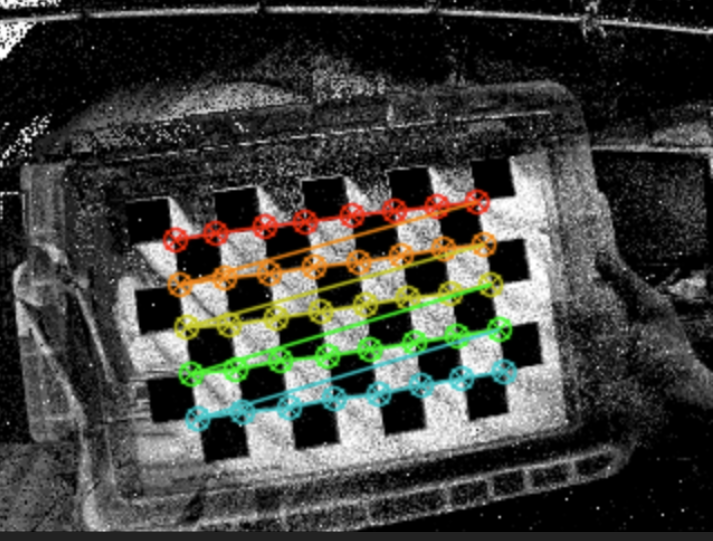
\includegraphics[width=0.62\textwidth]{images/Calibration/Calibration.png}
  \caption{Calibration initiale par échiquier dans une image reconstruite à partir des événements.}
  \label{fig:calibration-intrinseque}
\end{figure}

J'ai donc développé une mire adaptée au capteur: des disques lumineux
clignotent sur un écran fixe et produisent directement les événements utiles.
La grille est asymétrique afin de lever les ambiguïtés d'orientation, comme
l'illustre la \figref{fig:calibration-mire-concept}. Les événements sont
accumulés dans une image d'activité, puis les disques sont détectés et associés
à leurs positions physiques connues. Leurs centres image alimentent ensuite la
calibration OpenCV \cite{opencv-calib3d}.

\begin{figure}[H]
  \centering
  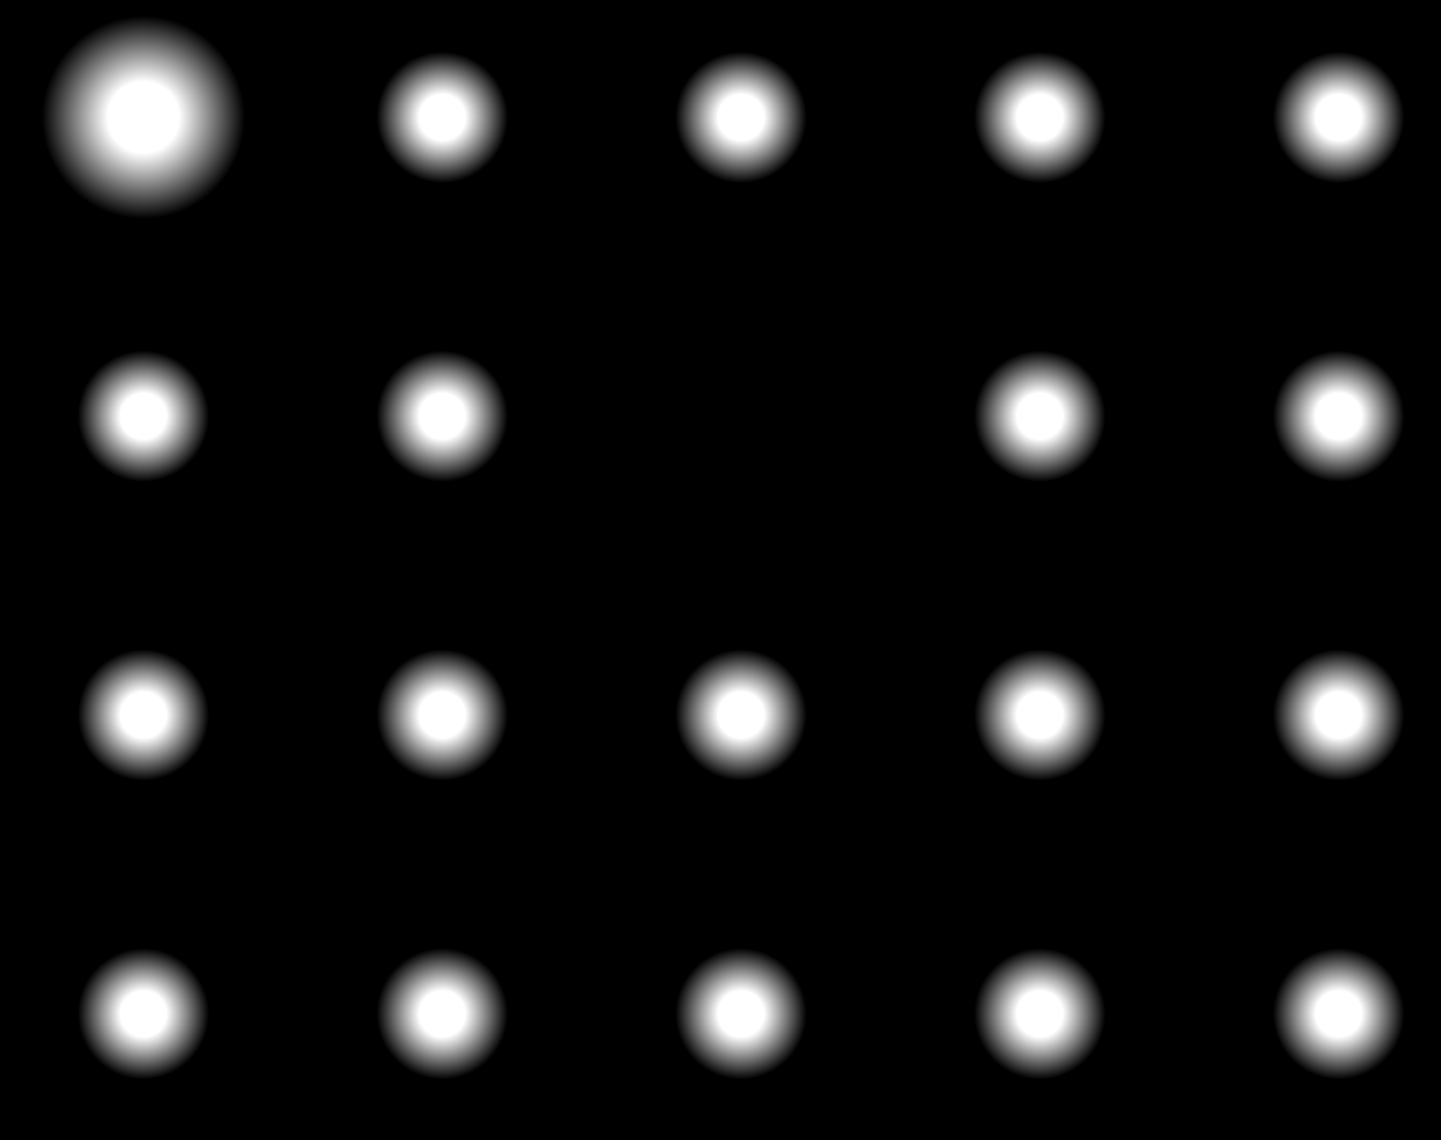
\includegraphics[width=0.58\textwidth]{images/Calibration/mire_concept.png}
  \caption{Mire asymétrique de disques clignotants utilisée pour la calibration événementielle.}
  \label{fig:calibration-mire-concept}
\end{figure}

Une cible plane observée uniquement de face contraint mal la focale: une focale
plus grande compensée par une distance plus élevée peut produire une image très
proche. Les acquisitions ont donc été réparties en position, en distance et en
inclinaison. La \figref{fig:poses-intrinseques} montre que le jeu retenu contient
bien des vues obliques et plusieurs distances. Il reste toutefois concentré au
centre de l'image et dominé par des inclinaisons modérées; une calibration
ultérieure gagnerait à mieux couvrir les bords du capteur.

L'inclinaison n'est donc pas un motif d'exclusion en elle-même. Une acquisition
est exploitable lorsque les disques restent distincts, entièrement visibles et
correctement associés à la géométrie de la mire. Une vue oblique apporte même
une information importante sur la perspective. À l'inverse, multiplier des
vues presque identiques de face augmente le nombre de points sans lever
l'ambiguïté entre focale et distance.

\begin{figure}[H]
  \centering
  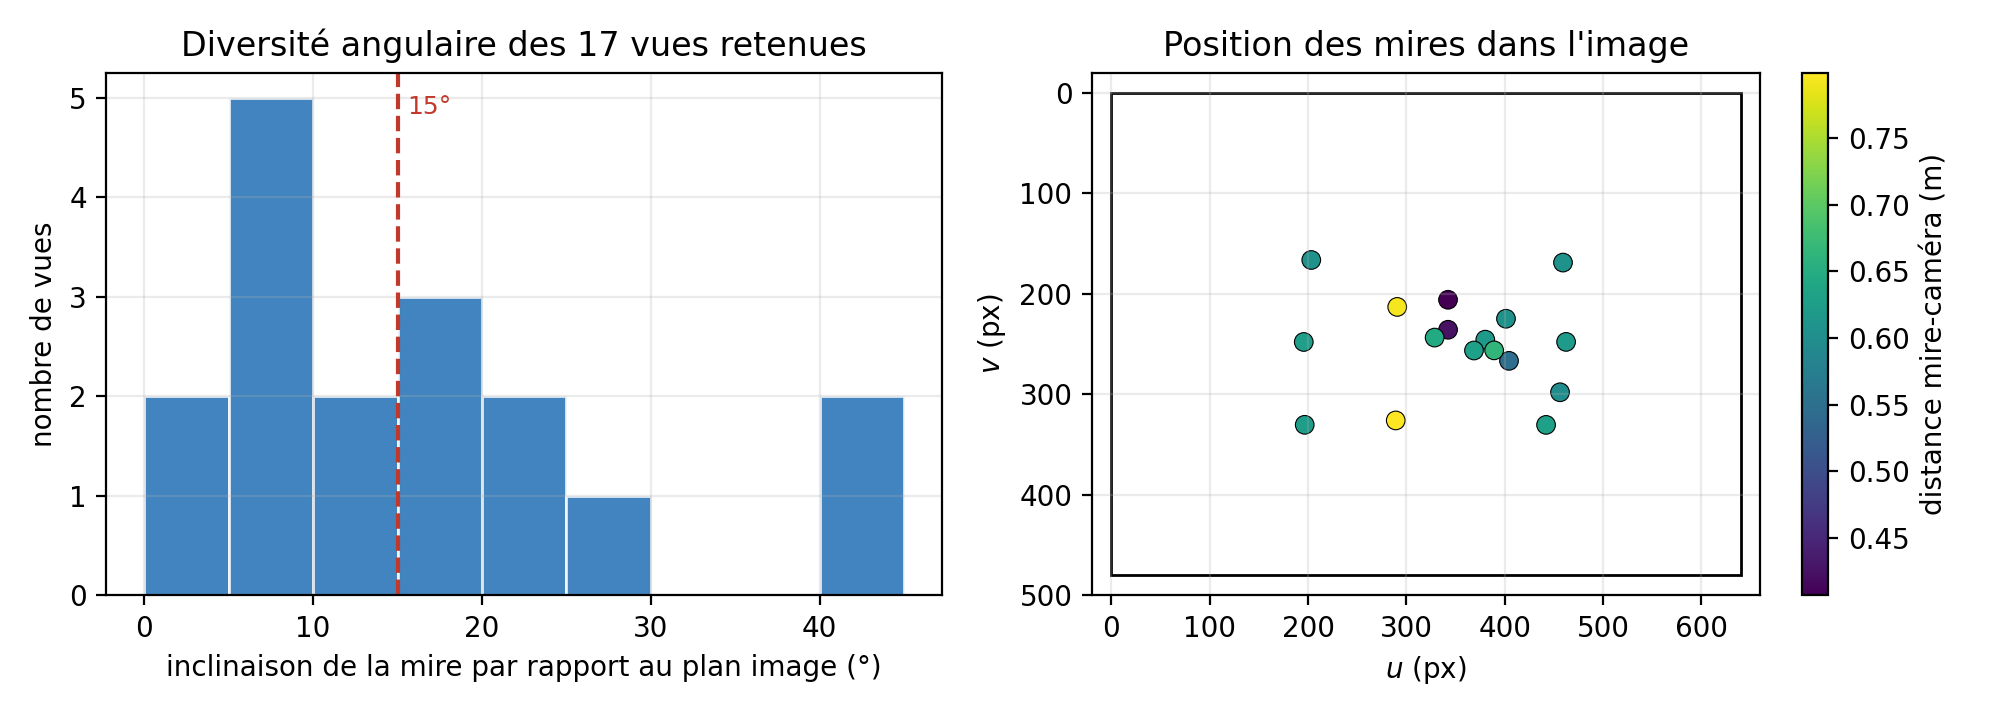
\includegraphics[width=\textwidth]{images/Calibration/poses_intrinseques.png}
  \caption{Répartition des poses utilisées pour la calibration intrinsèque: inclinaison de la mire, position dans l'image et distance à la caméra. Le trait rouge à \(15^\circ\) sert de repère pour visualiser la part des poses peu inclinées.}
  \label{fig:poses-intrinseques}
\end{figure}

La calibration retenue atteint une erreur de reprojection RMS de
\(0{,}149~\text{px}\). Ses paramètres, utilisés pour la correction de
distorsion et l'estimation de profondeur, sont donnés dans le
tableau~\ref{tab:intrinsic-sets}. Les deux procédures ne peuvent pas être
comparées directement, car l'optique a été modifiée entre leurs acquisitions;
leurs RMS respectives indiquent seulement la qualité d'ajustement sur deux jeux
de données différents.

\begin{table}[H]
  \centering
  \caption{Paramètres de la calibration intrinsèque retenue pour la DVXplorer.}
  \label{tab:intrinsic-sets}
  \begin{tabular}{rrrrrrr}
    \toprule
    \(f_x\) & \(f_y\) & \(c_x\) & \(c_y\) & \(k_1\) & \(k_2\) & RMS \\
    \midrule
    \(526{,}4\) & \(525{,}8\) & \(331{,}3\) & \(242{,}7\) & \(-0{,}402\) & \(0{,}170\) & \(0{,}149~\text{px}\) \\
    \bottomrule
  \end{tabular}
\end{table}

Ces paramètres ont une influence directe sur le résultat principal du système.
Pour la méthode Trace, la profondeur est proportionnelle à la focale effective
et inversement proportionnelle à la largeur apparente. Au premier ordre, leur
propagation peut s'écrire:

\begin{equation}
\frac{\Delta Z}{Z}
\simeq
\frac{\Delta f_{\text{eff}}}{f_{\text{eff}}}
-
\frac{\Delta w_{px}}{w_{px}}.
\label{eq:propagation-intrinseques-trace}
\end{equation}

Une focale surestimée produit ainsi un biais d'échelle sur toutes les
profondeurs, tandis qu'une mauvaise correction de distorsion déplace les
événements et modifie localement la largeur du ruban. La calibration intrinsèque
n'est donc pas seulement une étape préparatoire: elle fixe l'échelle métrique
de la trajectoire. Cette relation explique aussi pourquoi la comparaison des
deux méthodes de perception en simulation utilise les paramètres de la caméra
virtuelle et non ceux mesurés sur la DVXplorer réelle.

Un contrôle indépendant a été réalisé avec une cible carrée qui n'a pas servi à
l'estimation. Il donne une erreur RMS de \(0{,}13~\text{px}\) et une erreur
moyenne d'espacement de \(0{,}16~\text{mm}\), ce qui confirme la cohérence de
la calibration retenue. Ce test n'a pas pu être répété sur l'ancien réglage
optique; il valide donc la nouvelle calibration sans établir de comparaison
directe avec la procédure iniVation. La \figref{fig:intrinsic-mire-script}
montre le montage et une sortie de ce contrôle.

Ce contrôle complète l'erreur de reprojection de calibration. Cette dernière
mesure l'accord avec les données ayant servi à calculer les paramètres, alors
que la cible carrée introduit une autre géométrie et n'intervient pas dans
l'optimisation. L'accord observé sur ses espacements apporte donc une
vérification plus proche de l'usage attendu, qui consiste à convertir une
distance connue dans l'image en grandeur métrique.

\begin{figure}[H]
  \centering
  \begin{minipage}{0.48\textwidth}
    \centering
    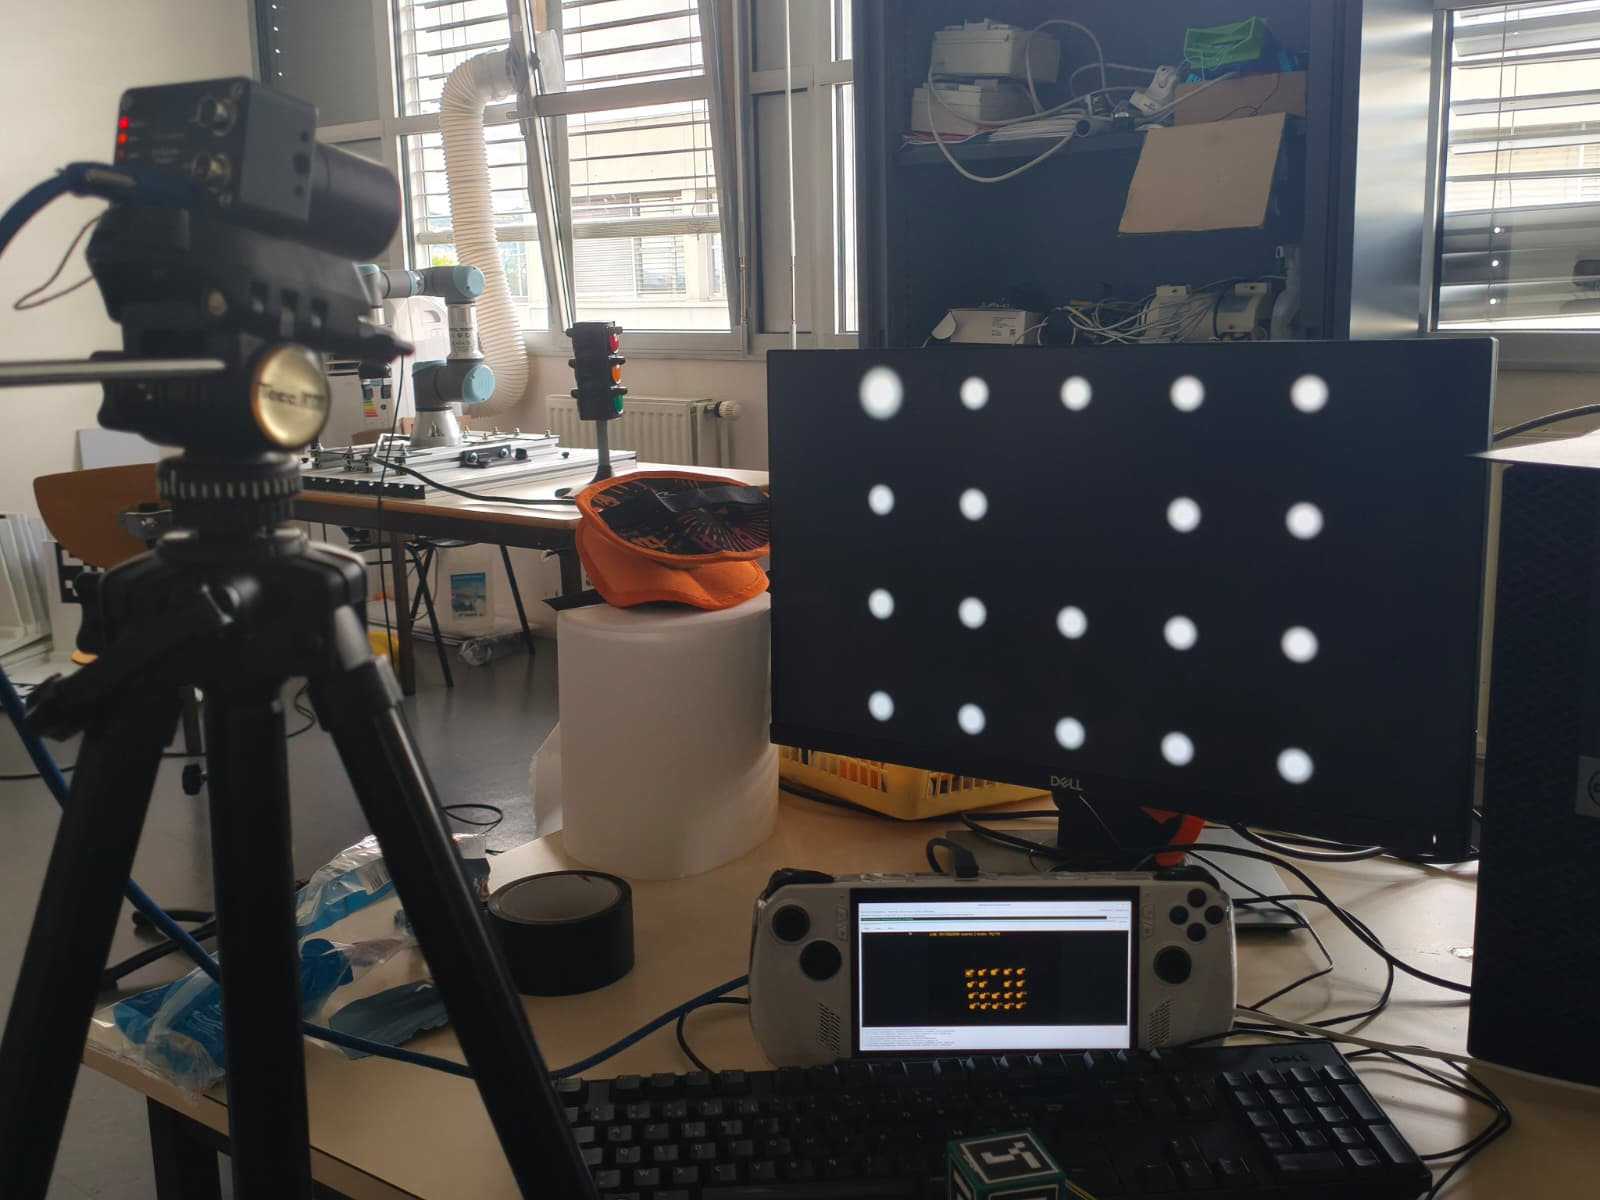
\includegraphics[width=\linewidth]{images/Calibration/Calibration_setup_ecran.jpeg}
  \end{minipage}
  \hfill
  \begin{minipage}{0.48\textwidth}
    \centering
    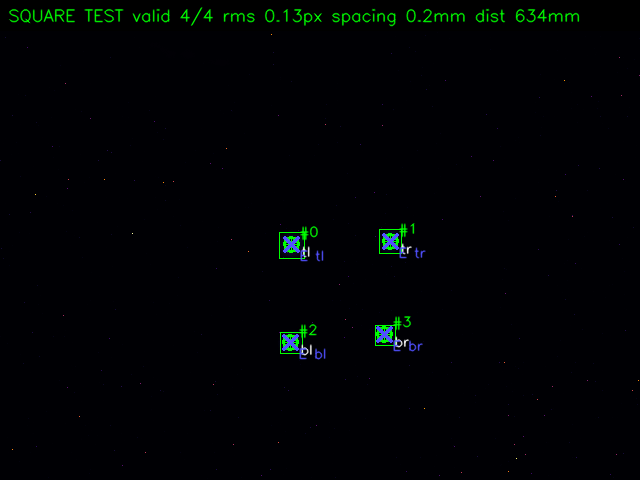
\includegraphics[width=\linewidth]{images/Calibration/square_test_20260611_110401_090251.png}
  \end{minipage}
  \caption{Calibration intrinsèque par mire événementielle. À gauche, la caméra observe une mire clignotante affichée sur écran; à droite, le test carré vérifie la cohérence de la calibration obtenue.}
  \label{fig:intrinsic-mire-script}
\end{figure}

\section{Méthode par circle fitting}

\subsection{Signal événementiel et polarités}

Une caméra événementielle transmet un événement lorsqu'un pixel détecte une
variation suffisante de luminosité:

\begin{equation}
e = (x, y, t, p),
\label{eq:evenement}
\end{equation}

où \(x\) et \(y\) sont les coordonnées du pixel, \(t\) son timestamp et \(p\)
la polarité, positive pour une augmentation de luminosité et négative pour une
diminution. Sur une balle en mouvement, les deux polarités apparaissent sur des
bords opposés, comme le montre la \figref{fig:event-ball-zoom}. Cette structure
aide à distinguer la balle du bruit.

\begin{figure}[H]
  \centering
  
\includegraphics[width=0.3\textwidth]{\detokenize{images/Algo_Cricle_Fitting/ball_events_zoom.png}}
  \caption{Événements produits par une balle en mouvement: polarité positive en bleu et négative en rouge.}
  \label{fig:event-ball-zoom}
\end{figure}

Si les événements sont accumulés trop longtemps, le contour instantané devient
une trace allongée. La durée d'observation doit donc fournir assez de points
sans mélanger trop de positions successives.

\subsection{Pipeline de l'algorithme}

La méthode par \emph{circle fitting} considère que la balle est une sphère dont la projection dans l'image peut être approchée par un cercle. L'idée est de détecter les événements appartenant probablement à la balle, d'ajuster un cercle sur ces points, puis d'utiliser le rayon apparent pour calculer la profondeur. La \figref{fig:algo-fitting-circle} résume les étapes principales de cette chaîne de traitement et l'information produite par chacune; une version détaillée des étapes internes est donnée dans l'annexe~\ref{ann:pipeline-circle}.

\begin{figure}[H]
  \centering
  \resizebox{\textwidth}{!}{%
  \begin{tikzpicture}[
      font=\small,
      block/.style={draw, rounded corners=2pt, align=center, text width=3.0cm, minimum height=1.2cm},
      source/.style={block, fill=blue!8},
      prep/.style={block, fill=cyan!8},
      estimate/.style={block, fill=orange!12},
      output/.style={block, fill=green!10},
      arrow/.style={-{Latex[length=2.5mm]}, thick},
      flow/.style={font=\footnotesize\itshape, midway, above}
    ]
    \node[source] (events) at (0,0) {Flux d'événements\\caméra ou séquence};
    \node[prep] (window) at (5.8,0) {Filtrage du bruit et\\fenêtre récente};
    \node[prep] (sample) at (11.6,0) {Échantillonnage et\\correction de distorsion};
    \node[prep] (dbscan) at (17.4,0) {Regroupement spatial\\DBSCAN};

    \node[estimate] (circle) at (17.4,-3.2) {Ajustement du cercle et\\validations: polarités,\\symétrie, points aberrants};
    \node[output] (pose) at (11.6,-3.2) {Pose 3D par\\projection inverse};
    \node[output] (traj) at (5.8,-3.2) {Régression de trajectoire\\et publication ROS 2};

    \draw[arrow] (events) -- node[flow] {événements bruts} (window);
    \draw[arrow] (window) -- node[flow] {événements récents} (sample);
    \draw[arrow] (sample) -- node[flow] {points corrigés} (dbscan);
    \draw[arrow] (dbscan) -- node[flow, right=1mm, align=left] {clusters candidats} (circle);
    \draw[arrow] (circle) -- node[flow] {cercle \((u,v,r)\)} (pose);
    \draw[arrow] (pose) -- node[flow] {position 3D} (traj);
    \draw[arrow, dashed] (circle.east) -- ++(1.0,0) |- (dbscan.east);
    \node[font=\footnotesize\itshape, anchor=west, align=left] at (20.15,-1.6) {validation échouée:\\cluster suivant};
  \end{tikzpicture}}
  \caption{Pipeline simplifié de la détection 3D par circle fitting. Chaque flèche porte l'information transmise à l'étape suivante; lorsqu'une validation échoue, le candidat est rejeté et le cluster suivant est examiné.}
  \label{fig:algo-fitting-circle}
\end{figure}

Les événements récents sont filtrés, corrigés de la distorsion puis regroupés
par DBSCAN. Les points isolés sont rejetés et les groupes couvrant une durée
trop longue sont découpés en sous-tranches afin de retrouver une forme proche
d'un cercle instantané. Les détails de ces étapes sont donnés dans
l'annexe~\ref{ann:pipeline-circle}.

\subsection{Ajustement du cercle et validation}

Chaque groupe candidat fournit un centre image et un rayon apparent:

\begin{equation}
(u, v, r),
\label{eq:cercle-uvr}
\end{equation}

où \(u\) et \(v\) sont les coordonnées du centre et \(r\) le rayon en pixels.
Le candidat est conservé si le résidu du cercle est faible et si les deux
polarités présentent la structure opposée visible sur la
\figref{fig:event-ball-zoom}. Les points aberrants sont ensuite retirés avant
un second ajustement.

\begin{figure}[H]
  \centering
  
\includegraphics[width=0.88\textwidth]{\detokenize{images/Algo_Cricle_Fitting/Sortie_algo_2D.png}}
  \caption{Sortie 2D de la méthode par cercle: événements, groupes candidats, cercle retenu et trajectoire image.}
  \label{fig:sortie-algo-2d}
\end{figure}

\subsection{Détermination de la pose 3D}

En connaissant le rayon réel \(R\) de la balle et la focale \(f_x\), la profondeur est estimée à partir du rayon apparent:

\begin{equation}
Z = \frac{f_x R}{r}.
\label{eq:profondeur-cercle}
\end{equation}

La position 3D complète est ensuite calculée par projection inverse:

\begin{equation}
X = \frac{u - c_x}{f_x} Z,
\qquad
Y = \frac{v - c_y}{f_y} Z.
\label{eq:projection-inverse}
\end{equation}

La pose obtenue est exprimée dans le repère caméra puis convertie en mètres pour
la suite de la chaîne.

\subsection{Régression de trajectoire 3D}
\label{sec:regression-3d}

Chaque position 3D valide est ajoutée à l'historique. Les positions sont auparavant exprimées dans le repère de travail de l'interface, obtenu du repère caméra par permutation d'axes, et dans lequel \(Z\) est l'axe vertical. La trajectoire y est modélisée par des régressions simples:

\begin{equation}
X(t) = a_x t + b_x,
\qquad
Y(t) = a_y t + b_y,
\qquad
Z(t) = a_z t^2 + b_z t + c_z.
\label{eq:modele-trajectoire}
\end{equation}

Les axes horizontaux sont modélisés par des droites et l'axe vertical par une
parabole. Une pondération favorise les points récents et réduit l'influence des
mesures aberrantes. Les expressions complètes sont données dans
l'annexe~\ref{ann:regressions}.

\subsection{Limite principale: sensibilité du rayon}

La limite principale vient de la dépendance de la profondeur au seul rayon
apparent. Sa sensibilité vaut:

\begin{equation}
\frac{dZ}{dr} = -\frac{f_x R}{r^2} = -\frac{Z}{r}.
\label{eq:sensibilite-rayon}
\end{equation}

Ainsi, une erreur de \(1~\text{px}\) produit une erreur de profondeur d'environ
\(Z/r\), d'autant plus grande que la balle est loin et que son rayon en pixels
est faible. Le tableau~\ref{tab:depth-sensitivity} chiffre cet effet aux
distances de travail visées: à \(1{,}5~\text{m}\), la balle ne mesure que
sept pixels de rayon et un pixel d'erreur déplace déjà la profondeur de plus de
\(20~\text{cm}\), soit bien au-delà du rayon utile du filet.

\begin{table}[H]
  \centering
  \caption{Sensibilité de la profondeur à une erreur d'un pixel, pour la calibration retenue (\(f_x \approx 526~\text{px}\)) et une balle de rayon \(R = 20~\text{mm}\). La dernière colonne correspond à la même erreur commise sur une largeur, deux fois plus grande que le rayon.}
  \label{tab:depth-sensitivity}
  \small
  \begin{tabular}{rrrrr}
    \toprule
    \(Z\) & Rayon \(r\) & Largeur \(w\) & Erreur pour \(1~\text{px}\) sur \(r\) & Erreur pour \(1~\text{px}\) sur \(w\) \\
    \midrule
    \(1{,}0~\text{m}\) & \(10{,}5~\text{px}\) & \(21{,}1~\text{px}\) & \(9{,}5~\text{cm}\) & \(4{,}7~\text{cm}\) \\
    \(1{,}5~\text{m}\) & \(7{,}0~\text{px}\) & \(14{,}0~\text{px}\) & \(21{,}4~\text{cm}\) & \(10{,}7~\text{cm}\) \\
    \(2{,}0~\text{m}\) & \(5{,}3~\text{px}\) & \(10{,}5~\text{px}\) & \(38{,}0~\text{cm}\) & \(19{,}0~\text{cm}\) \\
    \bottomrule
  \end{tabular}
\end{table}

À haute vitesse, la traînée événementielle élargit de plus le cercle ajusté et
rapproche artificiellement la balle de la caméra. Ce défaut n'étant pas stable
d'un lancer à l'autre, une correction unique serait fragile. Il motive la
méthode Trace, qui mesure la largeur sur plusieurs coupes de la forme réellement
observée.

\section{Méthode par trace événementielle}

\subsection{Motivation}

Pour une balle rapide, l'information utile est répartie dans toute la trace
événementielle. La méthode proposée exploite cette forme allongée comme un
ruban et mesure sa largeur sur plusieurs coupes. La profondeur ne dépend donc
plus d'un seul cercle ajusté localement.

Ce choix n'est pas seulement pratique, il est géométrique. Pendant la fenêtre
d'accumulation \(\Delta t\), la balle parcourt une distance \(v\,\Delta t\)
dans l'image: la silhouette accumulée s'étire dans la direction du déplacement,
mais reste inchangée dans la direction perpendiculaire, où son étendue vaut
toujours le diamètre apparent. Le rayon d'un cercle ajusté sur ce nuage croît
donc avec la durée d'accumulation, alors que la largeur mesurée
perpendiculairement à la trajectoire en est indépendante au premier ordre.
Mesurer une largeur transversale, et non un rayon, revient à choisir la seule
dimension de la trace qui ne soit pas polluée par le mouvement.

S'y ajoute un argument statistique. Le rayon est estimé à partir d'un contour
souvent partiel et bruité, et une seule valeur sert alors pour toute la fenêtre.
La trace fournit au contraire plusieurs dizaines de coupes le long du même
déplacement, dont la dispersion peut être exploitée pour écarter les mesures
incohérentes. Enfin, la largeur vaut le double du rayon: d'après le
tableau~\ref{tab:depth-sensitivity}, une même erreur d'un pixel y produit deux
fois moins d'erreur de profondeur. Ces trois effets se cumulent et expliquent
l'écart mesuré plus loin entre les deux méthodes.

\begin{figure}[H]
  \centering
  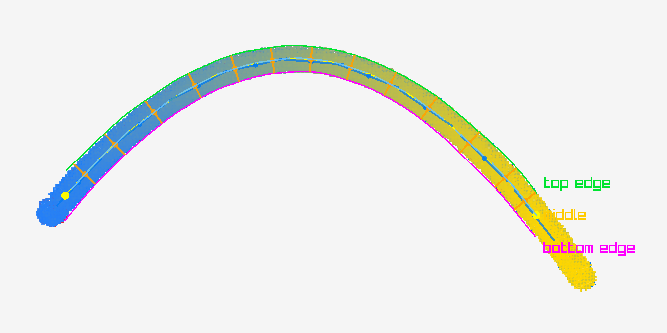
\includegraphics[width=0.70\textwidth]{images/Algo_Trace/Courbe1.png}
  \caption{Principe de la méthode Trace: bord haut en vert, ligne médiane en jaune, bord bas en magenta et mesures locales de largeur en orange.}
  \label{fig:trace-test}
\end{figure}

\subsection{Reconstruction du ruban}

Une fenêtre mobile sélectionne les événements proches de la trajectoire 2D. Une
analyse en composantes principales fournit ensuite la direction locale de la
trace. Le nuage est découpé le long de cette direction et, dans chaque portion,
les deux bords sont recherchés perpendiculairement. Les mesures isolées sont
rejetées avant d'ajuster le bord haut, la ligne médiane et le bord bas. La
\figref{fig:trace-ribbon} montre le résultat; les critères détaillés figurent
dans l'annexe~\ref{ann:trace-details}.


\begin{figure}[H]
  \centering
  \begin{tikzpicture}[font=\footnotesize, x=1cm, y=1cm]
    \begin{scope}[rotate=14]
      \fill[gray!8] (0,-0.5) rectangle (9,0.5);
      \draw[green!55!black, thick] (0,0.5) -- (9,0.5);
      \draw[magenta!80, thick] (0,-0.5) -- (9,-0.5);
      \draw[orange!90, thick, dashed] (0,0) -- (9,0);

      \foreach \x/\y in {0.35/0.31,0.7/-0.36,1.05/0.12,1.4/0.42,1.75/-0.28,2.1/0.05,2.45/-0.44,2.8/0.36,
                         3.15/-0.09,3.5/0.45,3.85/-0.31,4.2/0.18,4.55/-0.41,4.9/0.28,5.25/-0.14,5.6/0.4,
                         5.95/-0.35,6.3/0.09,6.65/-0.45,7.0/0.33,7.35/-0.2,7.7/0.44,8.05/-0.3,8.4/0.15}
        \fill[blue!55] (\x,\y) circle (1.1pt);

      \foreach \x in {1.8,3.6,5.4,7.2} \draw[gray!55, densely dotted] (\x,-1.0) -- (\x,1.0);
      \draw[gray!55, densely dotted] (2.7,-1.0) -- (2.7,1.0);
      \draw[gray!55, densely dotted] (4.5,-1.0) -- (4.5,1.0);
      \draw[gray!55, densely dotted] (6.3,-1.0) -- (6.3,1.0);

      \draw[{Latex[length=1.8mm]}-{Latex[length=1.8mm]}, thick] (4.05,-0.5) -- (4.05,0.5);
      \node[anchor=west, inner sep=1.5pt] at (4.12,0.0) {$w_j$};
      \node[anchor=north] at (4.05,-1.02) {bin $j$};

      \draw[-{Latex[length=2.2mm]}, thick] (8.6,-1.35) -- ++(1.1,0) node[below right, inner sep=1.5pt] {$s$, direction $d$};
      \draw[-{Latex[length=2.2mm]}, thick] (8.6,-1.35) -- ++(0,1.1) node[above, inner sep=1.5pt] {$h$, normale $n$};
    \end{scope}
    \node[anchor=west, green!45!black] at (0.2,3.45) {bord haut};
    \node[anchor=west, orange!80!black] at (0.2,3.05) {ligne médiane};
    \node[anchor=west, magenta!80] at (0.2,2.65) {bord bas};
  \end{tikzpicture}
  \caption{Géométrie du ruban. Les événements sont exprimés dans le repère local de la trace, \(s\) le long de la direction principale \(d\) et \(h\) selon la normale \(n\). La trace est découpée en bins le long de \(s\); dans chaque bin, les deux bords soutenus donnent la largeur locale \(w_j\), et leur milieu la ligne médiane. La largeur, mesurée perpendiculairement au déplacement, ne dépend pas de la durée d'accumulation, contrairement à la longueur de la trace.}
  \label{fig:trace-geometrie}
\end{figure}

La \figref{fig:trace-geometrie} fixe les notations. Le repère local de la
trace est défini par sa direction principale \(d\), estimée par analyse en
composantes principales, et par la normale \(n\) associée. Chaque événement y
est repéré par sa position \(s\) le long du déplacement et par sa position
\(h\) en travers du ruban. Le découpage en bins ramène alors un problème 2D
difficile à une suite de problèmes 1D: dans chaque bin, il suffit de trouver les
deux extrémités du paquet de valeurs \(h\), et un bord n'est retenu que s'il
est soutenu par plusieurs événements voisins, afin qu'un événement isolé ne
devienne pas à lui seul le bord de la balle.

Cette représentation locale sépare deux informations qui seraient mélangées
dans les coordonnées de l'image. La coordonnée longitudinale indique la
progression de la balle au cours de la fenêtre temporelle, tandis que la
coordonnée transversale décrit sa largeur apparente. La direction de la trace
peut ainsi évoluer sans imposer qu'elle soit horizontale ou verticale dans
l'image.

La reconstruction suit trois opérations complémentaires:
\begin{enumerate}
  \item les événements récents associés à la balle sont isolés et la direction
  dominante du déplacement est estimée;
  \item la trace est découpée en portions spatiales, dans lesquelles les deux
  bords doivent être soutenus par plusieurs événements voisins;
  \item les portions incohérentes avec la forme locale du ruban sont retirées,
  puis les bords et la ligne médiane sont ajustés sur les mesures conservées.
\end{enumerate}

Cette construction évite qu'un événement isolé devienne à lui seul un bord de
la balle. Elle permet également de conserver plusieurs mesures de largeur le
long d'un même mouvement, au lieu de réduire immédiatement tout le nuage à un
cercle unique.

\begin{figure}[H]
  \centering
  
\includegraphics[width=0.66\textwidth]{\detokenize{images/Algo_Trace/Screenshot from 2026-06-04 17-32-17.png}}
  \caption{Vue Trace dans l'interface pour une balle lancée vers la caméra. Les événements récents sont colorés selon le temps, puis le ruban est reconstruit avec un bord haut, une ligne médiane, un bord bas et plusieurs mesures de largeur.}
  \label{fig:trace-ribbon}
\end{figure}


\subsection{Conversion 3D par largeur de trace}

La conversion 3D repose sur le même principe géométrique que le circle fitting, mais la grandeur mesurée n'est plus le rayon d'un cercle. Pour plusieurs instants de la trace, la méthode mesure une largeur perpendiculaire à la ligne médiane. Cette largeur est utilisée comme diamètre apparent de la balle:

\begin{equation}
Z = \frac{f_{\text{eff}}D}{w_{px}},
\label{eq:profondeur-trace}
\end{equation}

où \(D\) est le diamètre réel de la balle et \(w_{px}\) la largeur mesurée en pixels, corrigée comme décrit plus bas. Comme la largeur n'est pas forcément horizontale ou verticale dans l'image, la méthode utilise une focale effective dans la direction de mesure. En notant \(n = (n_x, n_y)\) le vecteur unitaire de l'image perpendiculaire à la ligne médiane du ruban, c'est-à-dire la direction dans laquelle la largeur est mesurée, cette focale vaut:

\begin{equation}
f_{\text{eff}} =
\sqrt{(f_x n_x)^2 + (f_y n_y)^2}.
\label{eq:focale-effective}
\end{equation}

Le centre image \((u,v)\) de la mesure permet ensuite de retrouver les coordonnées caméra:

\begin{equation}
X = \frac{(u-c_x)Z}{f_x},
\qquad
Y = \frac{(v-c_y)Z}{f_y}.
\label{eq:projection-trace}
\end{equation}

Dans l'affichage 3D, ces coordonnées sont ensuite remappées dans le repère utilisé par l'interface. Les positions 3D aberrantes sont filtrées par sauts temporels et par résidu de trajectoire. Le résultat final est donc une suite de points 3D, puis une trajectoire ajustée sur ces points. Les sorties obtenues avec cette conversion sont présentées dans la section~\ref{chap:simulation-validation}, où la simulation fournit une vérité terrain pour comparer directement l'estimation à la position réelle de la balle.

\subsection{Correction du biais de largeur apparente}

La profondeur donnée par~\eqref{eq:profondeur-trace} est inversement
proportionnelle à la largeur mesurée. Une légère sous-estimation de cette
largeur suffit donc à placer la balle trop loin de la caméra. Ce phénomène est
peu visible lorsque la balle occupe une vingtaine de pixels, mais devient
prépondérant à longue distance, lorsque son diamètre apparent n'est plus que de
quelques pixels.

L'étude des séquences simulées a permis d'identifier l'origine principale du
biais. Les événements décrivent des centres de pixels et les bords soutenus du
ruban restent légèrement à l'intérieur de la silhouette réelle. De plus, lorsque
les événements sont peu denses, la distance entre les derniers échantillons du
bord augmente. Une correction identique pour toutes les distances ne suffit
donc pas. La largeur \(w_{px}\) utilisée dans~\eqref{eq:profondeur-trace} n'est donc pas la largeur brute du ruban, mais une largeur corrigée:

\begin{equation}
w_{px} = w_{\text{brut}} +
2\left(\delta_{px}+\kappa\,\bar{s}_{\text{bord}}\right),
\label{eq:correction-largeur-trace}
\end{equation}

où \(\delta_{px}\) compense la quantification liée au centre des pixels,
\(\bar{s}_{\text{bord}}\) représente l'espacement médian des événements près
des bords et \(\kappa\) adapte la correction à la densité observée. Les valeurs
utilisées et le calcul complet sont donnés dans
l'annexe~\ref{ann:trace-details}. La même correction est employée pour les
séquences nominales et lointaines: elle dépend de l'information mesurée sur le
ruban, pas d'une distance supposée de la balle.

\begin{figure}[H]
  \centering
  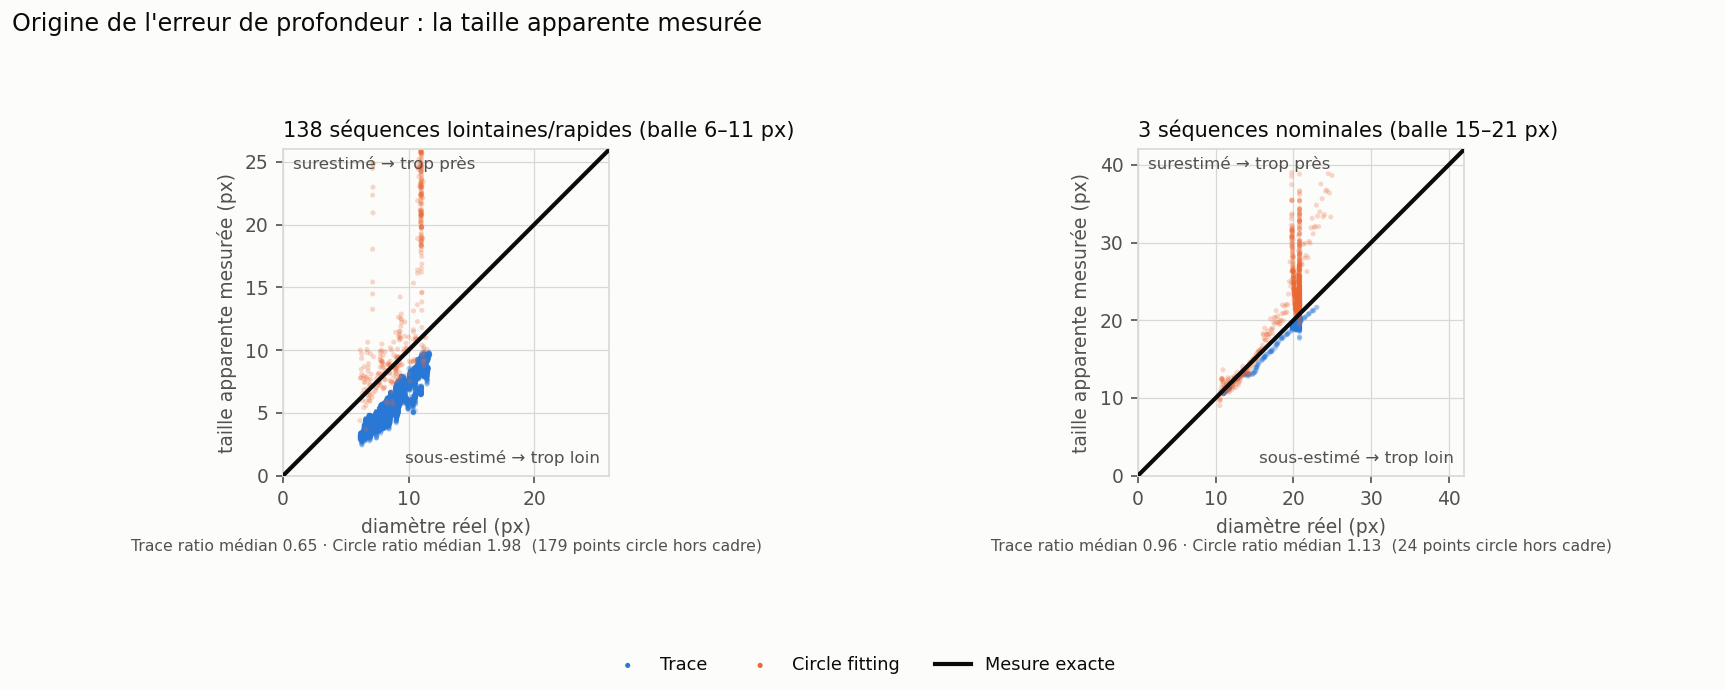
\includegraphics[width=0.93\textwidth]{images/Benchmark_Trace_Circle/biais_taille_apparente_avant.png}
  \vspace{0.3em}
  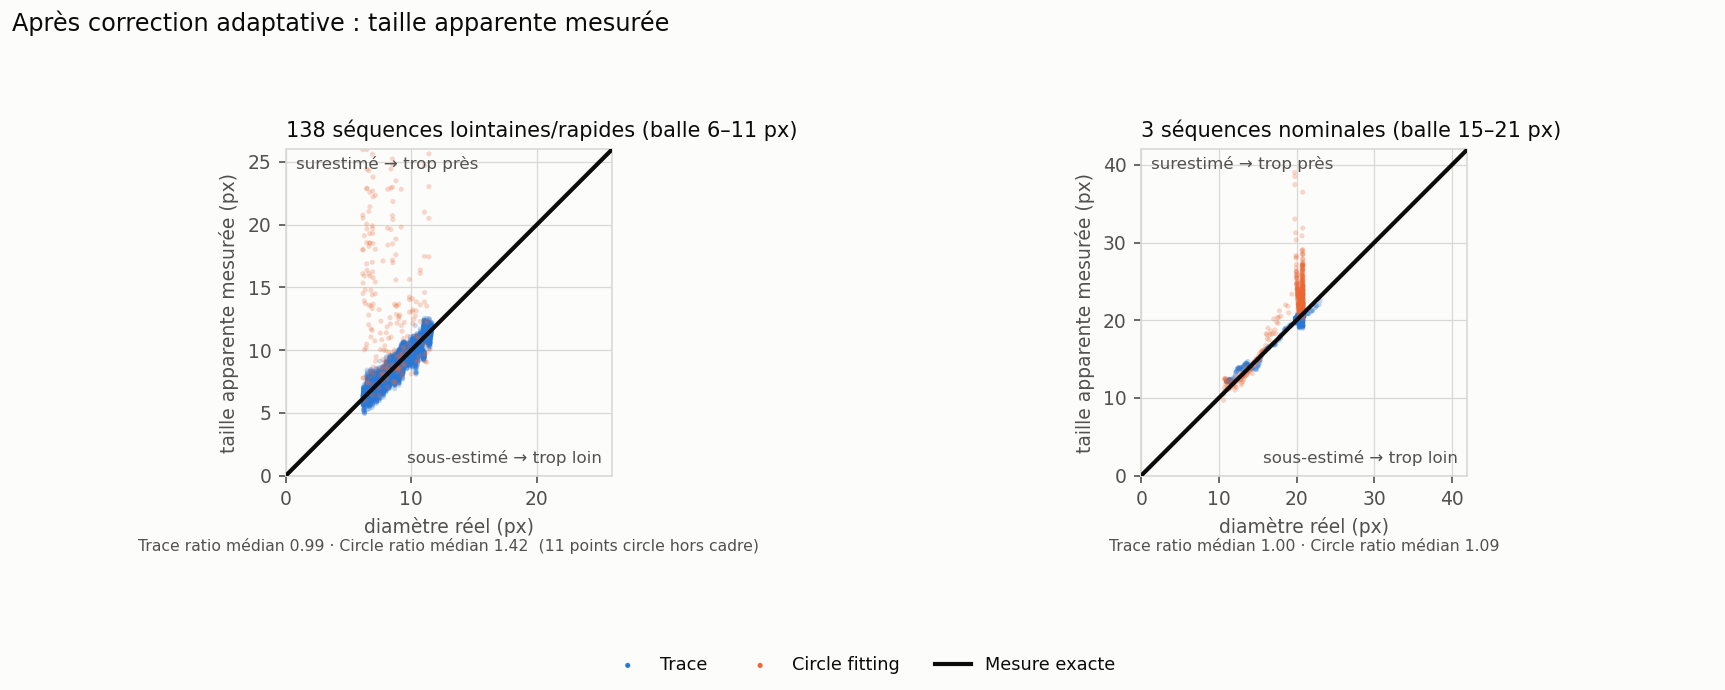
\includegraphics[width=0.93\textwidth]{images/Benchmark_Trace_Circle/biais_taille_apparente_apres.png}
  \caption{Taille apparente mesurée avant (en haut) et après (en bas) la correction des bords. La diagonale noire représente une mesure exacte. La correction rapproche les mesures Trace de cette diagonale dans les régimes nominal et lointain, sans chercher à corriger le circle fitting.}
  \label{fig:correction-largeur-trace}
\end{figure}

Le tableau~\ref{tab:ablation-correction-trace} isole l'effet de cette étape. En
régime nominal, le gain est modéré car la largeur brute est déjà proche de la
référence. À longue distance, la correction supprime en revanche l'essentiel
du biais d'échelle: le rapport entre largeur mesurée et largeur réelle passe de
\(0{,}65\) à \(0{,}99\). Le taux de détection ne change pas, ce qui montre que
l'amélioration vient bien de l'estimation géométrique des bords et non d'un
assouplissement du détecteur.

\begin{table}[H]
  \centering
  \caption{Effet de la correction de largeur sur la méthode Trace.}
  \label{tab:ablation-correction-trace}
  \begin{tabular}{L{0.25\textwidth}rrr}
    \toprule
    Régime & RMSE 3D avant & RMSE 3D après & Rapport largeur après \\
    \midrule
    Nominal & \(0{,}058~\text{m}\) & \(\mathbf{0{,}045~\text{m}}\) & \(1{,}00\) \\
    Lointain et rapide & \(1{,}716~\text{m}\) & \(\mathbf{0{,}157~\text{m}}\) & \(0{,}99\) \\
    \bottomrule
  \end{tabular}
\end{table}


\subsection{Régression pondérée de trajectoire}

La suite de positions 3D reste bruitée, en particulier sur l'axe de profondeur.
Une régression temporelle est donc ajustée sur les mesures conservées. Les
coordonnées horizontales sont modélisées par des fonctions affines, tandis que
la coordonnée verticale autorise un terme quadratique pour représenter la
gravité. Ce modèle volontairement simple peut être actualisé rapidement et ne
cherche pas à reproduire tous les effets aérodynamiques d'un lancer.

La pondération accorde davantage d'importance aux points récents et cohérents.
Les mesures anciennes contribuent encore à stabiliser l'estimation, mais une
valeur ponctuellement éloignée de la tendance influence moins la trajectoire
finale. Au début du lancer, peu de points sont disponibles et la courbure
verticale reste mal contrainte; la prédiction se stabilise ensuite à mesure que
la fenêtre s'enrichit. Les expressions de la régression sont regroupées dans
l'annexe~\ref{ann:regressions}.

\subsection{Bilan de la méthode Trace}

La méthode reste sensible à la largeur mesurée et à la densité d'événements,
mais elle exploite une information mieux adaptée aux mouvements rapides. Son
intérêt ne vient pas seulement d'une disponibilité accrue: la reconstruction
du ruban permet aussi d'expliquer puis de corriger le principal biais de
profondeur.

Son domaine de validité mérite cependant d'être précisé, car il découle
directement du principe retenu. La méthode suppose d'abord un déplacement
suffisant pendant la fenêtre d'accumulation: une balle lente produit une trace
courte, dont la direction principale est mal définie et dont les coupes se
confondent. Elle suppose ensuite un déplacement majoritairement transversal;
une balle arrivant exactement dans l'axe de la caméra ne parcourt presque
aucune distance dans l'image et ne forme donc pas de ruban exploitable. Elle
suppose enfin une densité d'événements suffisante pour que les bords soient
soutenus, condition qui se dégrade avec la distance et que la correction de
largeur ne compense que partiellement. Dans le cas d'usage visé, une balle
lancée vers le robot mais vue de côté par la caméra, ces trois conditions sont
réunies; elles rappellent en revanche que la méthode est adaptée à une
situation, et non universelle. La section suivante vérifie quantitativement
cet avantage contre une vérité terrain commune aux deux méthodes.

\section{Simulation et validation}
\label{chap:simulation-validation}

\subsection{Séquences simulées et vérité terrain}

Des lancers ont été générés avec Isaac Sim \cite{nvidia-isaac-sim}, puis les
images converties en événements avec \texttt{v2e}
\cite{v2e-github,v2e-paper}. La position réelle de la balle et sa projection
image sont conservées comme vérité terrain. Les paramètres de génération sont
donnés dans l'annexe~\ref{ann:sequences}.

\begin{figure}[H]
  \centering
  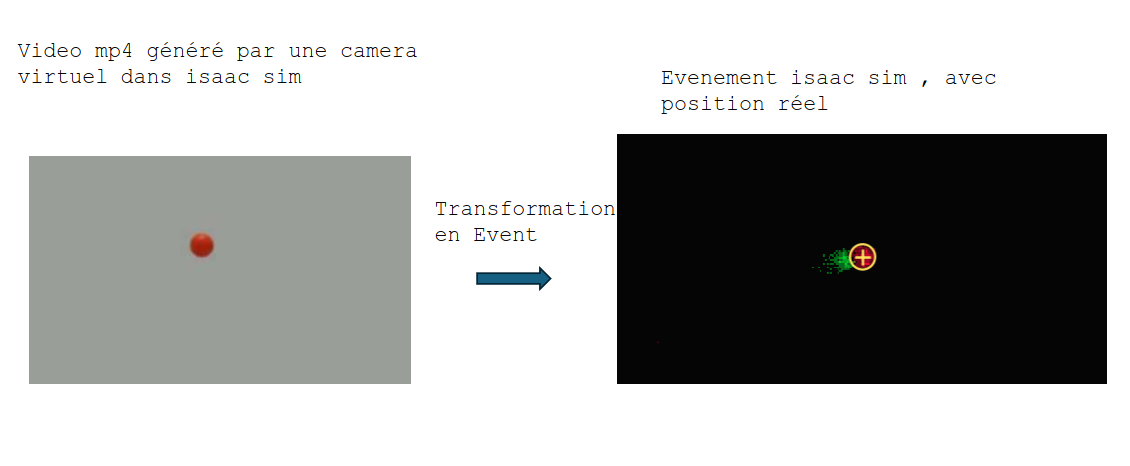
\includegraphics[width=0.64\textwidth]{images/V2e.png}
  \caption{Conversion d'une séquence simulée en flux événementiel avec \texttt{v2e} \cite{v2e-github,v2e-paper}.}
  \label{fig:v2e-conversion}
\end{figure}

Cette validation porte sur trois séquences nominales, proches de la zone
d'interception, et sur un lot de \(138\) lancers plus lointains et rapides. Elle
permet de mesurer séparément les erreurs dans l'image et en profondeur.

\subsection{Comparaison quantitative des deux méthodes}
\label{sec:comparaison-quantitative}

Chaque séquence est rejouée dans les deux chaînes avec les mêmes événements et
la même vérité terrain. Les deux méthodes utilisent les paramètres de la caméra
virtuelle, et non ceux de la DVXplorer réelle, puis chaque estimation est
comparée à la vérité terrain au même instant. Ce point n'est pas un détail de
mise en œuvre: la profondeur étant proportionnelle à la focale, appliquer par
mégarde la calibration de la caméra réelle multiplierait toutes les profondeurs
estimées par un facteur voisin de \(1{,}5\), sans produire le moindre symptôme
visible dans l'image. Le régime nominal couvre des
profondeurs de \(1{,}0\) à \(1{,}4~\text{m}\); le régime lointain s'étend de
\(1{,}8\) à \(3{,}4~\text{m}\), avec une balle de seulement \(6\) à
\(11~\text{px}\) de diamètre apparent.

Cinq grandeurs sont comparées. Le taux de détection est la proportion
d'instants où la méthode produit une pose 3D. Les RMSE 2D, de profondeur et 3D
mesurent les différentes composantes de l'erreur; le temps de calcul mesure le
coût moyen d'une estimation. Les résultats sont donnés dans le
tableau~\ref{tab:benchmark-trace-circle}.

\begin{table}[H]
  \centering
  \caption{Comparaison des deux méthodes contre la vérité terrain simulée, chacune à son meilleur point de fonctionnement. Le temps de calcul est le coût processeur moyen par estimation produite, mesuré pendant le rejeu hors ligne; la meilleure valeur de chaque colonne est en gras.}
  \label{tab:benchmark-trace-circle}
  \begin{tabular}{lrrrr}
    \toprule
    & \multicolumn{2}{c}{Régime nominal} & \multicolumn{2}{c}{Régime lointain et rapide} \\
    \cmidrule(lr){2-3}\cmidrule(lr){4-5}
    Métrique & Trace & Circle fitting & Trace & Circle fitting \\
    \midrule
    Taux de détection  & \(\mathbf{0.73}\)  & \(0.47\)  & \(\mathbf{0.74}\)  & \(0.013\) \\
    RMSE 2D            & \(\mathbf{5.4}~\text{px}\) & \(9.2~\text{px}\) & \(\mathbf{2.2}~\text{px}\) & \(7.3~\text{px}\) \\
    RMSE profondeur    & \(\mathbf{0.043}~\text{m}\) & \(0.128~\text{m}\) & \(\mathbf{0.153}~\text{m}\) & \(0.643~\text{m}\) \\
    RMSE 3D            & \(\mathbf{0.045}~\text{m}\) & \(0.136~\text{m}\) & \(\mathbf{0.157}~\text{m}\) & \(0.685~\text{m}\) \\
    Temps de calcul    & \(1.7~\text{ms}\) & \(\mathbf{0.008}~\text{ms}\) & \(1.7~\text{ms}\) & \(\mathbf{0.008}~\text{ms}\) \\
    \bottomrule
  \end{tabular}
\end{table}

La méthode Trace est environ trois fois plus précise en 3D en régime nominal et
fournit davantage d'estimations. Son temps de calcul de \(1{,}7~\text{ms}\)
reste compatible avec la période de commande de \(16{,}7~\text{ms}\). Le circle
fitting est beaucoup plus rapide, mais son erreur 3D et son faible taux de
détection à distance le rendent moins adapté à l'interception.

La \figref{fig:benchmark-nominal} montre que les deux méthodes suivent la balle
dans l'image. Leur différence vient surtout de la taille apparente: le cercle la
surestime davantage, ce qui dégrade directement la profondeur.

\begin{figure}[H]
  \centering
  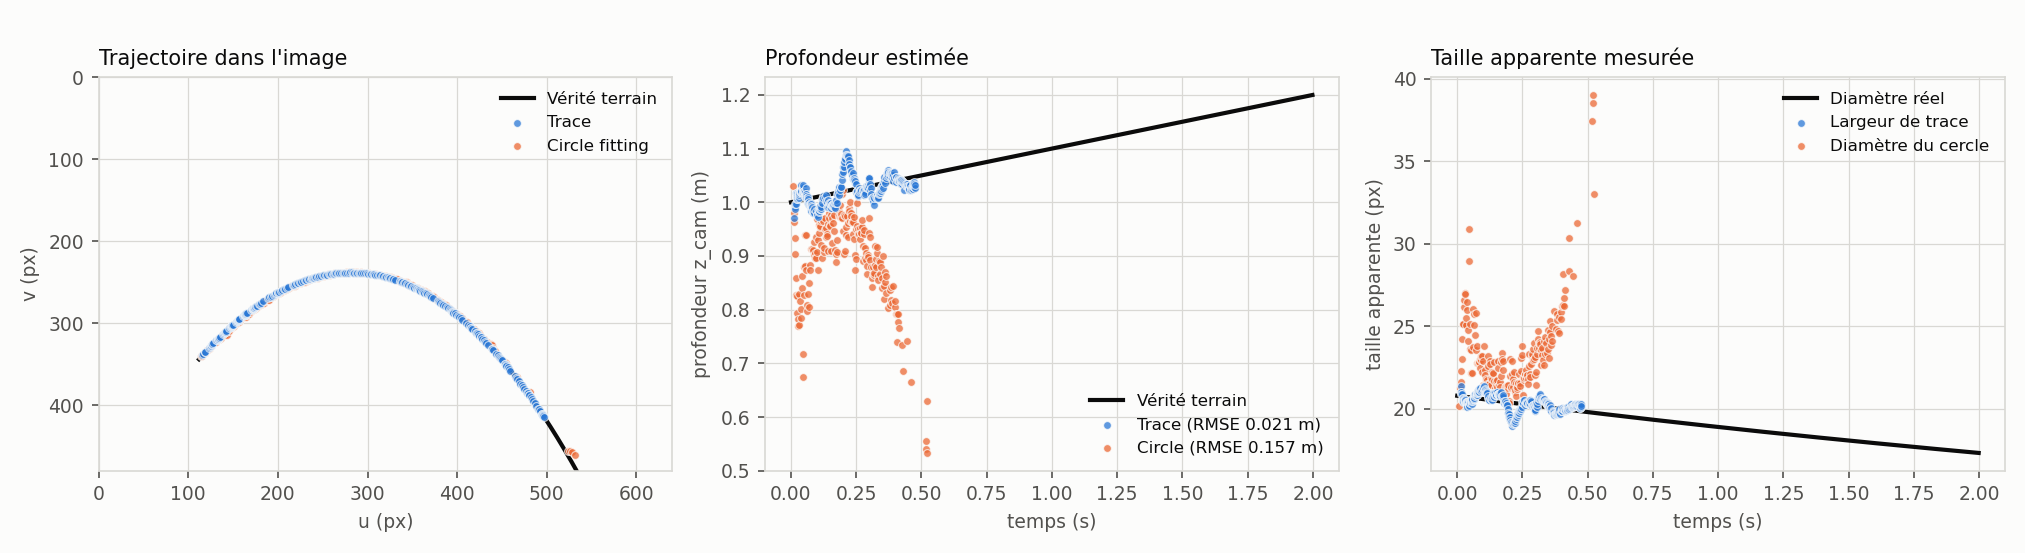
\includegraphics[width=\textwidth]{images/Benchmark_Trace_Circle/comparaison_nominal.png}
  \caption{Régime nominal (balle à environ \(1.0~\text{m}\)). De gauche à droite: trajectoire dans l'image, profondeur estimée et taille apparente mesurée, pour les deux méthodes comparées à la vérité terrain.}
  \label{fig:benchmark-nominal}
\end{figure}

À distance, la balle devient trop petite pour que la structure de polarités et
le rayon du cercle restent stables. La \figref{fig:benchmark-lointain} montre
alors une seule estimation par cercle, tandis que la trace reste disponible.

\begin{figure}[H]
  \centering
  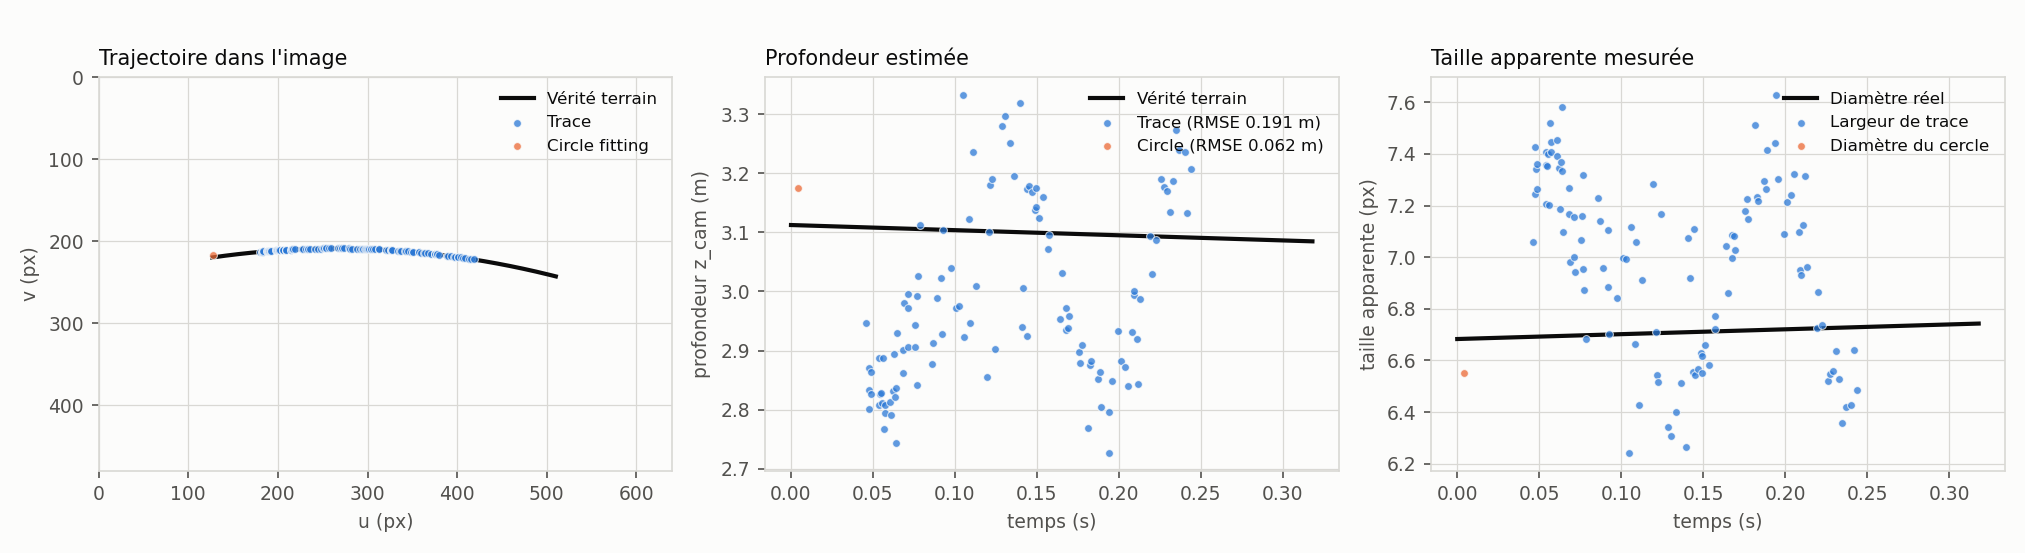
\includegraphics[width=\textwidth]{images/Benchmark_Trace_Circle/comparaison_lointain.png}
  \caption{Régime lointain et rapide (balle à environ \(3.1~\text{m}\), diamètre apparent de \(6.7~\text{px}\)). Le circle fitting ne fournit qu'une seule estimation sur toute la séquence, alors que la trace reste disponible en continu.}
  \label{fig:benchmark-lointain}
\end{figure}

La RMSE du circle fitting à distance doit être lue avec son taux de détection de
\(1{,}3~\%\): elle ne concerne que de rares estimations. La méthode Trace reste
elle aussi limitée à longue distance, car quelques dixièmes de pixel sur la
largeur entraînent déjà une erreur importante en profondeur.

\subsection{Interprétation des résultats}

Le taux de détection et la RMSE répondent à deux questions différentes. Le
premier indique pendant quelle part du vol une information est disponible; la
seconde mesure la qualité de cette information lorsqu'elle existe. Une méthode
peut donc présenter une erreur apparemment faible en ne conservant que quelques
instants faciles. C'est pourquoi le résultat lointain du circle fitting ne peut
pas être interprété indépendamment de son taux de détection de \(1{,}3~\%\).

Dans le régime nominal, la méthode Trace produit une position sur environ
\(73~\%\) des instants évalués et atteint une erreur 3D de \(4{,}5~\text{cm}\).
Le circle fitting est disponible moins d'une fois sur deux et son erreur atteint
\(13{,}6~\text{cm}\). Les trajectoires image de la
\figref{fig:benchmark-nominal} montrent pourtant que les deux méthodes localisent
globalement la balle dans le plan image. La différence provient principalement
de l'estimation de sa taille apparente, donc de la profondeur. Ce résultat
confirme qu'un suivi 2D visuellement correct n'est pas suffisant pour fournir
une position exploitable par le robot.

Le régime lointain rend ce phénomène plus sévère. Pour la séquence illustrée par
la \figref{fig:benchmark-lointain}, une erreur de \(1~\text{px}\) sur un diamètre
apparent de \(6{,}7~\text{px}\) représente environ \(15~\%\) de la mesure. Par
la relation inverse entre largeur et profondeur, cela peut déplacer la balle de
plusieurs dizaines de centimètres. La méthode Trace reste donc moins précise
qu'en régime nominal, mais elle conserve suffisamment de mesures pour ajuster
une trajectoire, contrairement au cercle.

Le coût de calcul conduit à une conclusion différente. Le circle fitting est
nettement plus rapide, mais les \(1{,}7~\text{ms}\) de Trace ne représentent
qu'environ un dixième de la période de décision de \(16{,}7~\text{ms}\). Dans le
cadre du cahier des charges, la précision et la continuité supplémentaires sont
donc obtenues sans compromettre la cadence visée. Ces mesures portent toutefois
sur le calcul de l'estimation seule; la latence complète jusqu'au mouvement du
robot est étudiée séparément lors des essais réels.

\subsection{Convergence de la trajectoire}

La \figref{fig:trace-convergence} superpose la trajectoire estimée à la vérité
terrain au fil d'un lancer du lot lointain. Les trois courbes bleues sont le
modèle de trajectoire ajusté sur une part croissante des mesures, tracé en trait
plein jusqu'au dernier point utilisé puis prolongé en pointillé. Sur la hauteur,
la parabole ajustée sur le premier tiers du vol s'écarte fortement dès qu'on
l'extrapole, alors que l'ajustement complet suit la référence. Sur la
profondeur, les estimations restent dispersées d'environ \(\pm 5~\text{cm}\)
autour de la valeur réelle: la régression retrouve la bonne pente mais conserve
un biais de l'ordre de \(2~\text{cm}\). Cette lecture sur un lancer unique
illustre ce que les RMSE du tableau~\ref{tab:benchmark-trace-circle} mesurent
sur l'ensemble du lot.

\begin{figure}[H]
  \centering
  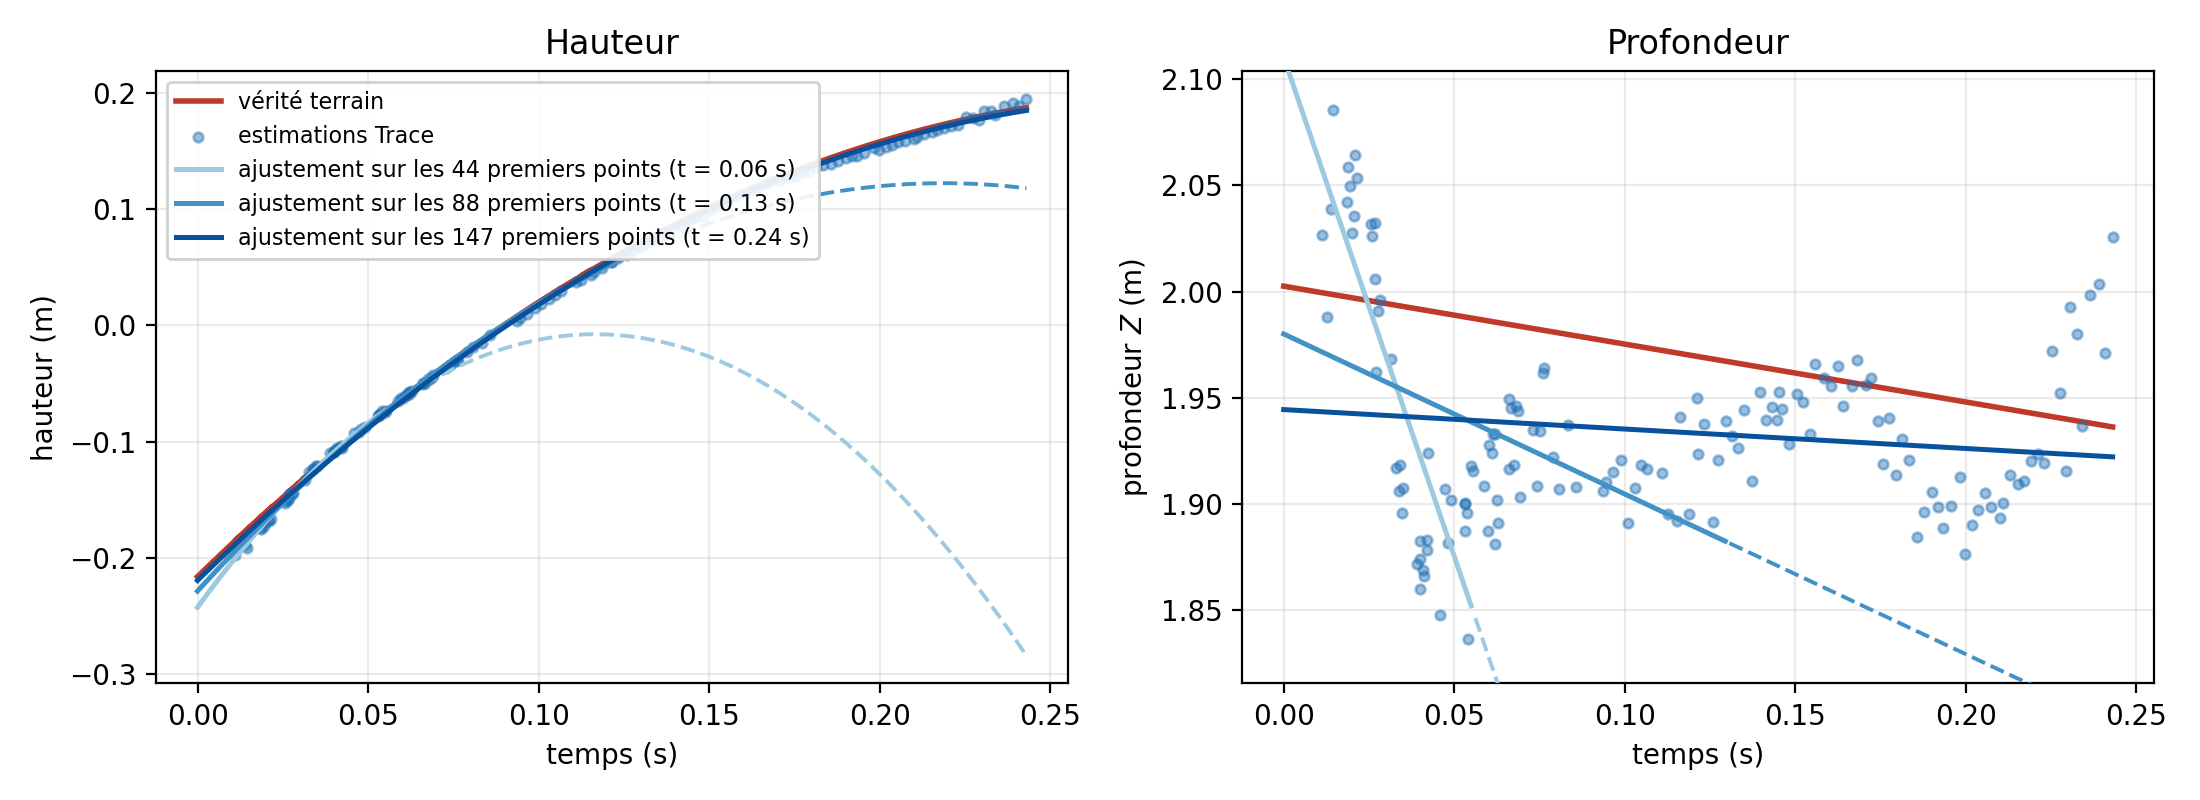
\includegraphics[width=\textwidth]{images/Algo_Trace/trace_convergence.png}
  \caption{Trajectoire Trace superposée à la vérité terrain, à gauche la hauteur et à droite la profondeur. Les points bleus sont les estimations instantanées, la courbe rouge la position réelle, et les trois courbes bleues les trajectoires ajustées sur une part croissante des mesures, en trait plein jusqu'au dernier point utilisé puis en pointillé en extrapolation. Séquence représentative du lot lointain, avec une balle d'environ \(10{,}5~\text{px}\) de diamètre apparent à \(1{,}95~\text{m}\).}
  \label{fig:trace-convergence}
\end{figure}

\subsection{Portée et limites de cette validation}

La simulation fournit une référence exacte, mais ne reproduit pas entièrement
l'éclairage et le bruit du capteur réel. Ces résultats comparent donc les deux
méthodes dans un cadre contrôlé; les essais réels du chapitre suivant évaluent
la chaîne complète.

\chapter{Intégration robotique et contrôle}
\label{chap:robotique}

\section{Calibration extrinsèque par mire événementielle}
\label{chap:calibration-extrinseque}

\subsection{Principe et montage}

Les méthodes précédentes estiment la balle dans le repère de la caméra. La
calibration extrinsèque cherche donc la transformation fixe entre ce repère et
la base du robot:

\begin{equation}
{}^{B}T_{C}.
\label{eq:transfo-base-camera}
\end{equation}

Le robot déplace un smartphone fixé à son effecteur et affichant la mire
clignotante déjà utilisée pour la calibration intrinsèque. La cinématique du
robot donne la pose de l'écran dans la base, tandis que la caméra observe la
mire. Plusieurs orientations et distances fournissent alors les contraintes
nécessaires pour estimer une transformation unique.

\begin{figure}[H]
  \centering
  \begin{minipage}{0.48\textwidth}
    \centering
    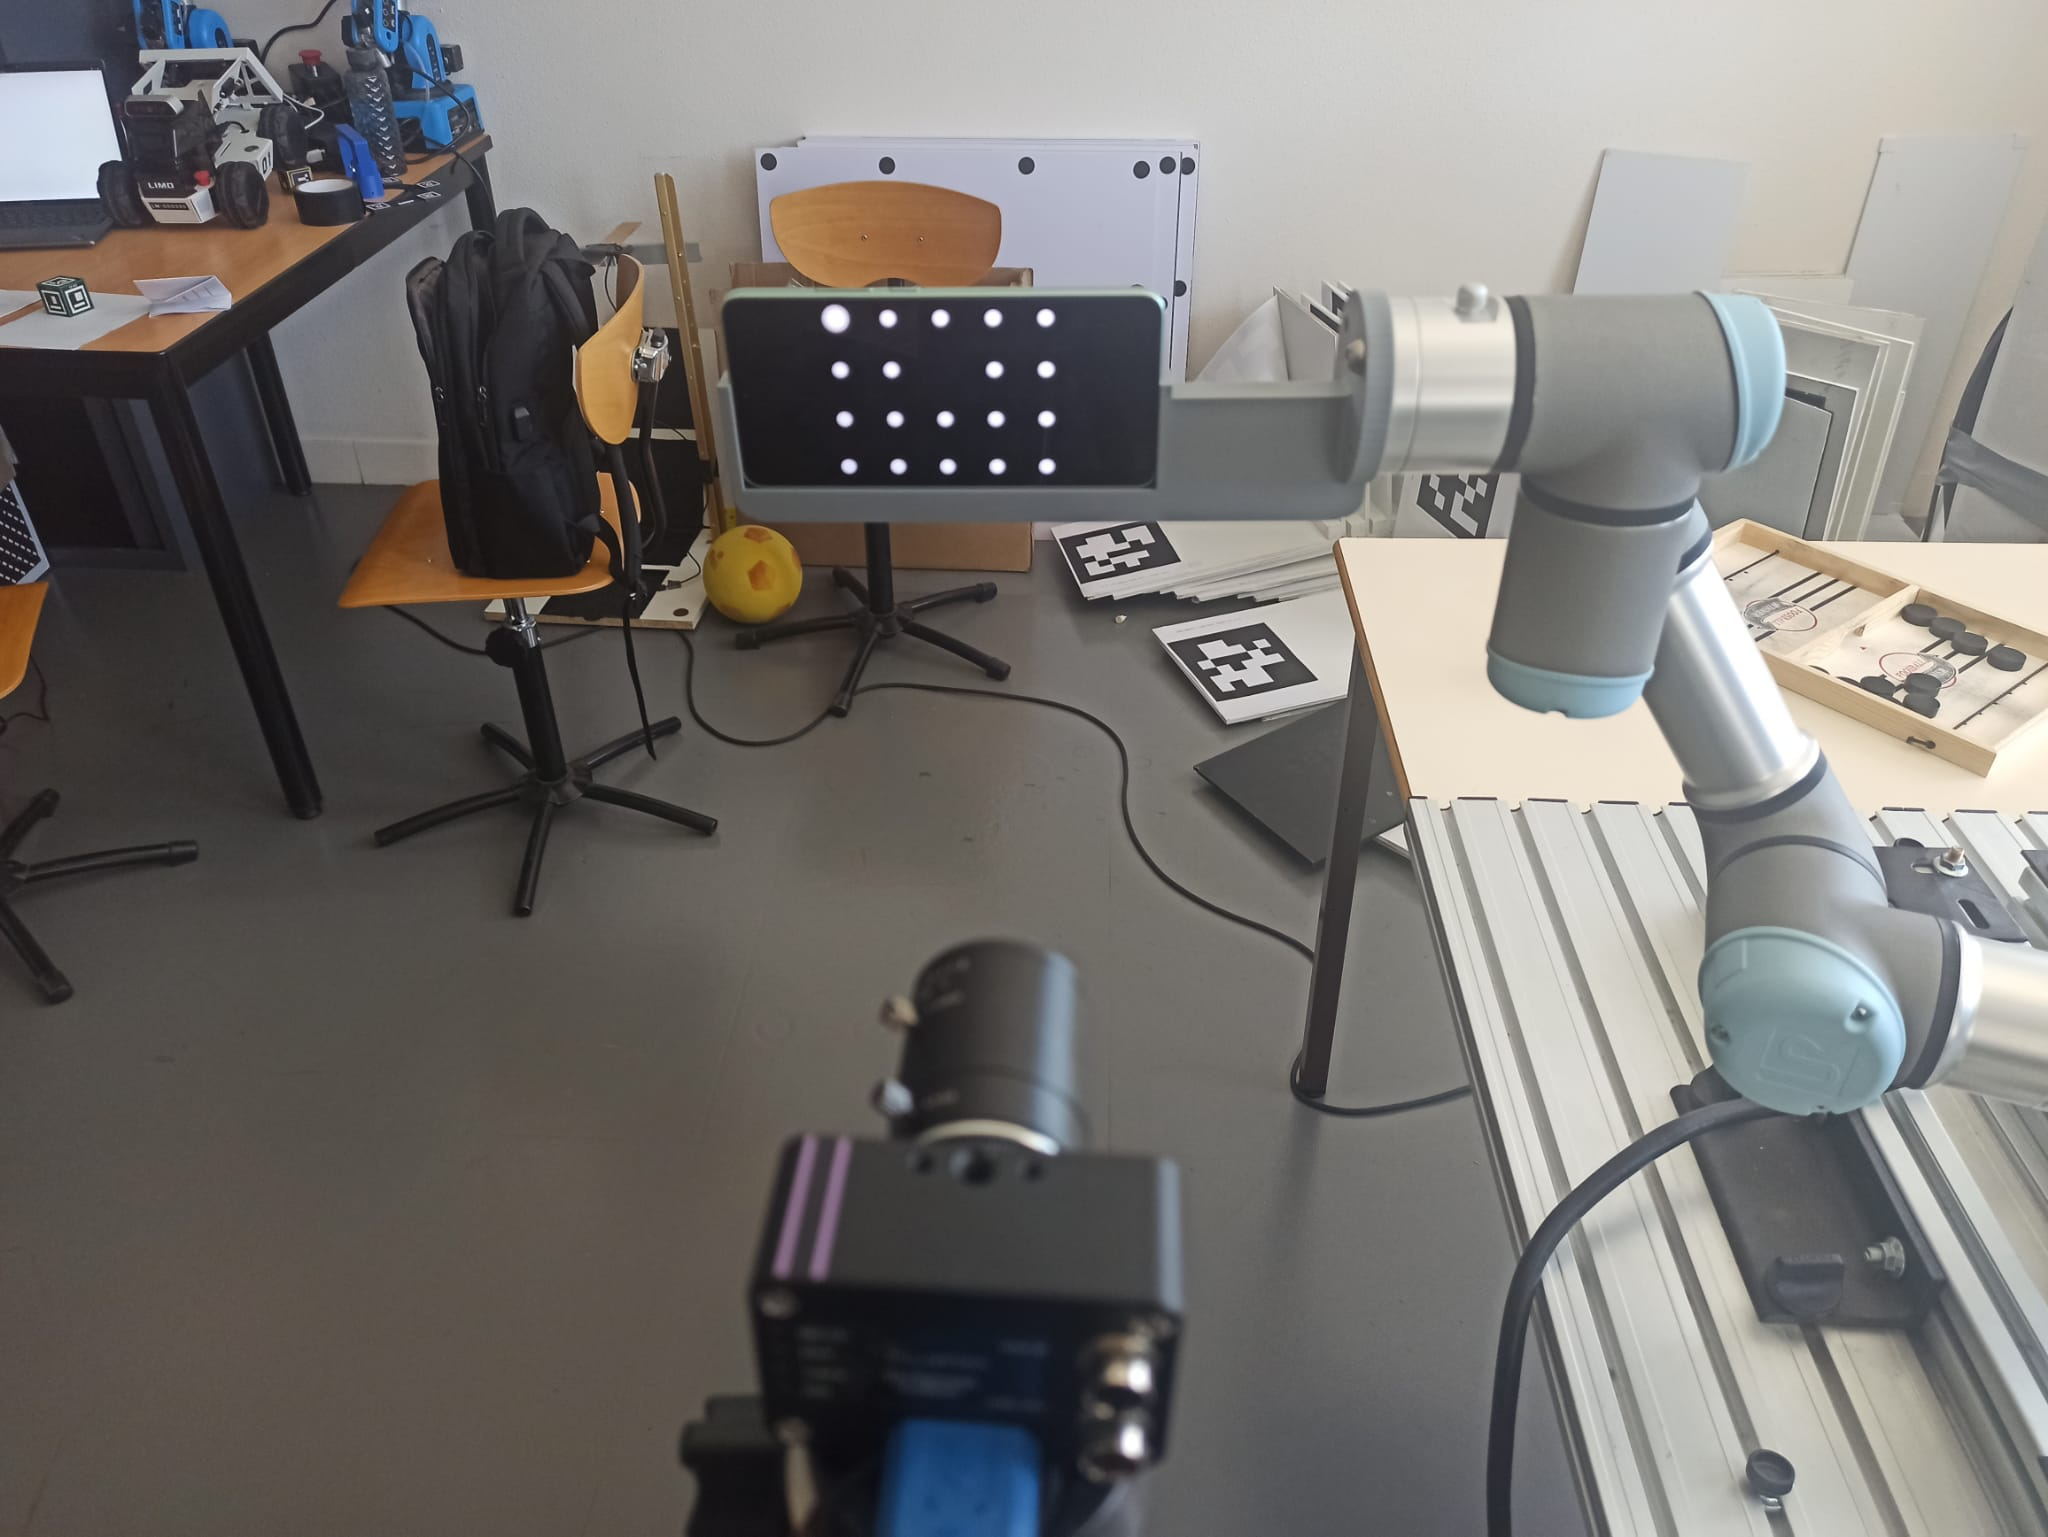
\includegraphics[width=\linewidth]{images/Calibration/Smartphone_Sur_Support.jpeg}
  \end{minipage}
  \hfill
  \begin{minipage}{0.48\textwidth}
    \centering
    
\includegraphics[width=\linewidth]{\detokenize{images/Calibration/Smartphone_Sur_Support_vue_coté.jpeg}}
  \end{minipage}
  \caption{Smartphone fixé à l'effecteur pour afficher la mire dynamique.}
  \label{fig:smartphone-support}
\end{figure}

\subsection{Repères et transformations}

Les repères \(B\), \(E\), \(S\) et \(C\) désignent respectivement la base du
robot, l'effecteur, la mire et la caméra. Pour une pose \(i\), la cinématique
donne \({}^{B}T_{E,i}\) et la géométrie du support donne \({}^{E}T_S\). La pose
de la mire dans la base vaut donc:

\begin{equation}
{}^{B}T_{S,i} = {}^{B}T_{E,i}\,{}^{E}T_S.
\label{eq:pose-mire-base}
\end{equation}

La caméra fournit en parallèle la pose \({}^{C}T_{S,i}\) à partir des centres
des disques, de leurs dimensions physiques et des paramètres intrinsèques. La
taille utile de l'écran a été mesurée afin de conserver une échelle métrique
correcte.

\begin{figure}[H]
  \centering
  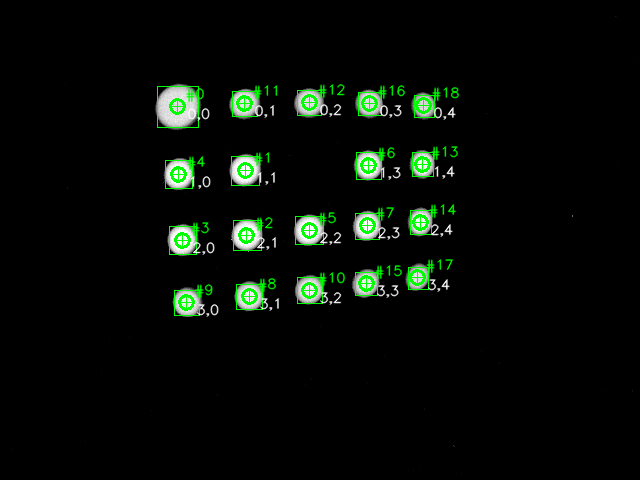
\includegraphics[width=0.64\textwidth]{images/Calibration/mire_overlay_vue_1.png}
  \caption{Détection et association des disques de la mire dans le flux événementiel.}
  \label{fig:mire-blob-output}
\end{figure}

\subsection{Calibration multi-poses}

La transformation finale est obtenue en minimisant l'erreur de reprojection sur
l'ensemble des poses et des points observés:

\begin{equation}
\min_{{}^{C}T_B}
\sum_{i,j}
\left\|
\pi\left({}^{C}T_B\,{}^{B}T_{S,i}\,P_j^S\right)
- \hat{\mathbf{u}}_{ij}
\right\|^2,
\label{eq:reprojection-globale}
\end{equation}

où \(\pi\) représente la projection caméra.

Les acquisitions couvrent plusieurs positions, distances et orientations de
l'écran. Une acquisition est conservée lorsque tous les disques sont détectés et
correctement associés, que le robot est immobile pendant la fenêtre
d'accumulation et que l'écran reste affiché en plein écran au format paysage,
condition nécessaire pour que sa géométrie métrique soit connue. Une inclinaison
suffisante est également requise: une cible plane vue presque de face admet deux
poses quasi équivalentes, si bien que ce sont les vues trop peu inclinées, et non
les vues obliques, qui doivent être écartées. La qualité de la solution est
ensuite contrôlée par l'erreur de reprojection et par une validation croisée
entre les poses.

\subsection{Résultats de la calibration physique caméra-robot}
\label{sec:resultats-handeye}

Le montage réel est visible sur la \figref{fig:handeye-setup-reel}. Le
smartphone est fixé au bout du UR3e et la caméra observe la mire depuis un
trépied fixe.

\begin{figure}[H]
  \centering
  \begin{minipage}{0.48\textwidth}
    \centering
    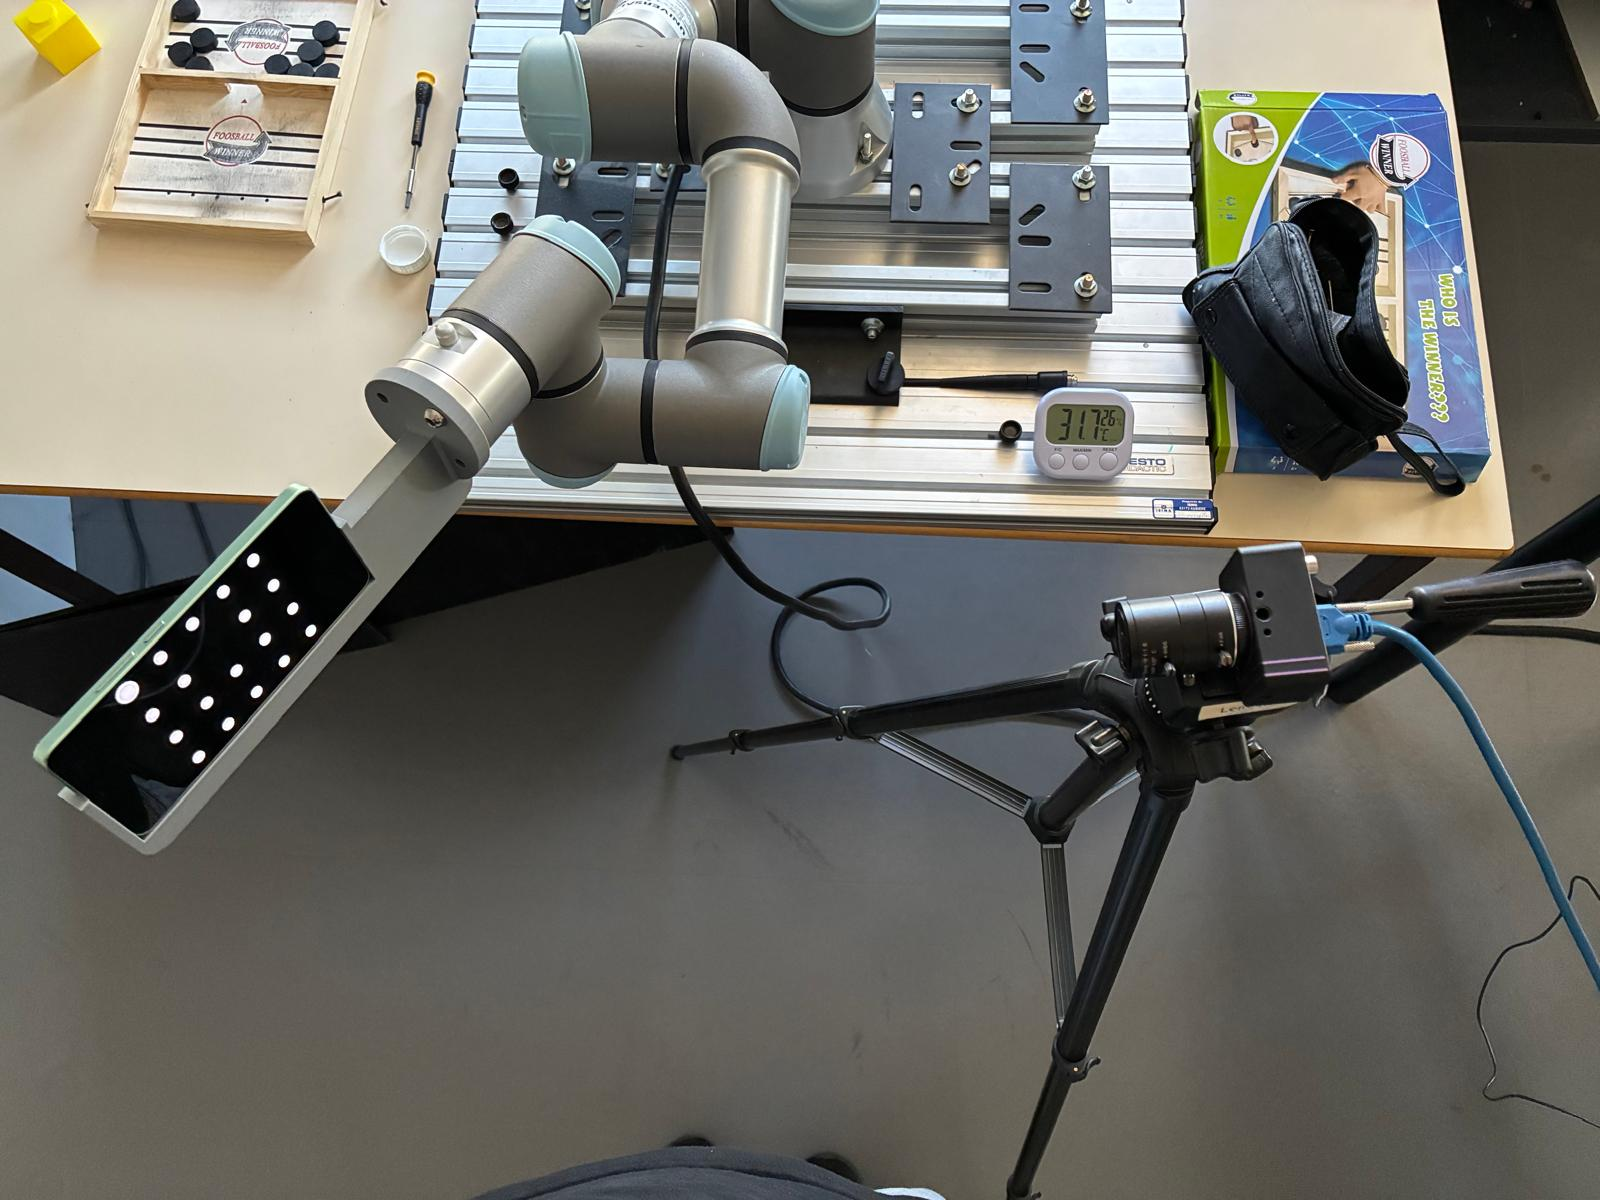
\includegraphics[width=\linewidth]{images/Calibration/Calibration_photo_setup.jpg}
  \end{minipage}
  \hfill
  \begin{minipage}{0.48\textwidth}
    \centering
    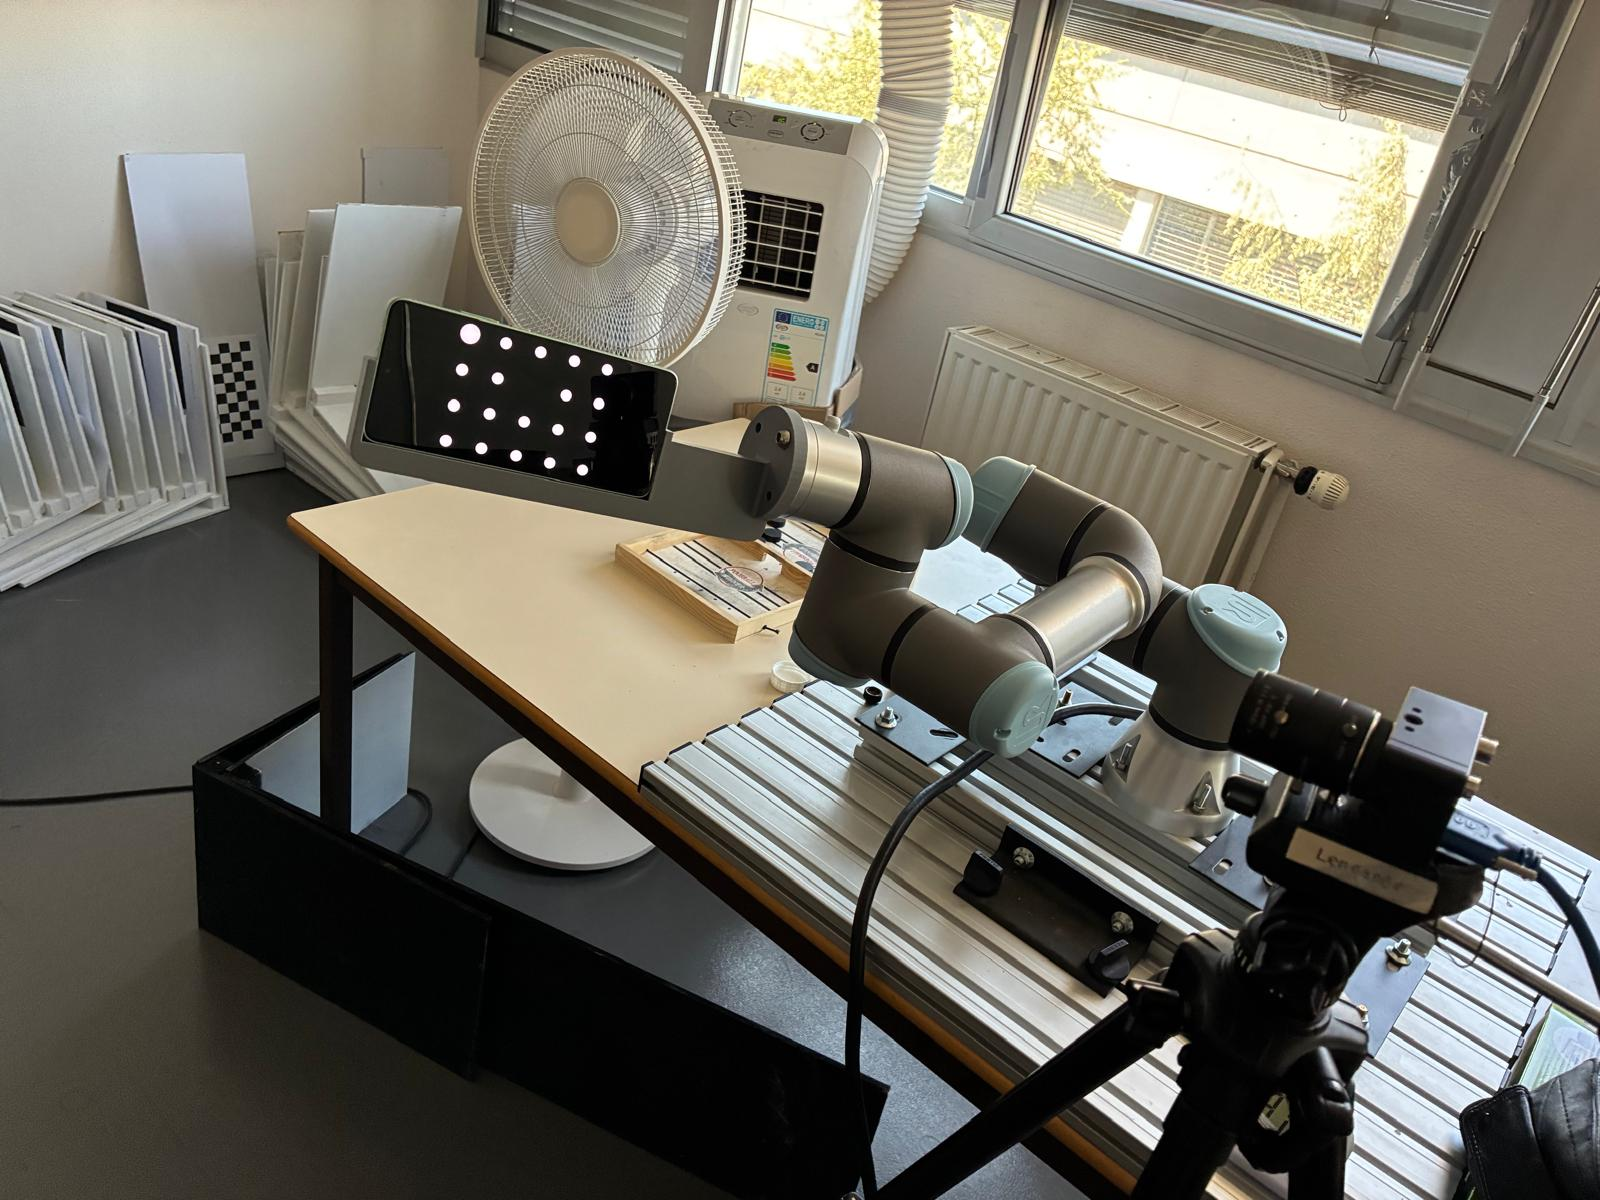
\includegraphics[width=\linewidth]{images/Calibration/Calibration_photo_setup2.jpg}
  \end{minipage}
  \caption{Montage réel de la calibration extrinsèque. Le smartphone affichant la mire clignotante est porté par le UR3e via le support imprimé en 3D, et la caméra événementielle observe la scène depuis un trépied fixe.}
  \label{fig:handeye-setup-reel}
\end{figure}

La solution obtenue présente un résidu moyen de \(1{,}11~\text{mm}\) en
translation et de \(0{,}27^\circ\) en rotation. L'erreur de reprojection vaut
\(0{,}98~\text{px}\) RMS. La validation croisée, qui retire successivement une
pose, déplace au maximum la solution de \(1{,}79~\text{mm}\) et
\(0{,}16^\circ\). Ces résultats indiquent une solution numériquement cohérente;
les valeurs complètes sont données dans l'annexe~\ref{ann:handeye}.

Ces indicateurs ne contrôlent pas exactement les mêmes propriétés. L'erreur de
reprojection vérifie que la transformation estimée explique correctement les
centres observés dans l'image. Les résidus en translation et en rotation
mesurent la cohérence des transformations obtenues à partir des différentes
poses. Enfin, la validation croisée vérifie que la solution ne dépend pas
fortement d'une acquisition particulière. Leur lecture conjointe est résumée
dans le tableau~\ref{tab:lecture-handeye}.

\begin{table}[H]
  \centering
  \caption{Lecture des principaux indicateurs de calibration caméra-robot.}
  \label{tab:lecture-handeye}
  \small
  \begin{tabular}{L{0.28\textwidth}L{0.18\textwidth}L{0.44\textwidth}}
    \toprule
    Indicateur & Valeur obtenue & Information apportée \\
    \midrule
    Reprojection RMS & \(0{,}98~\text{px}\) & Accord entre la géométrie estimée et les observations dans l'image. \\
    Résidu moyen & \(1{,}11~\text{mm}\), \(0{,}27^\circ\) & Cohérence des poses dans un même repère caméra-robot. \\
    Variation maximale en validation croisée & \(1{,}79~\text{mm}\), \(0{,}16^\circ\) & Stabilité de la solution lorsqu'une acquisition est retirée. \\
    \bottomrule
  \end{tabular}
\end{table}

Une faible erreur de reprojection ne constitue cependant pas, à elle seule, une
mesure physique indépendante de la position de la caméra. Les mêmes mesures
servent à estimer puis à contrôler la transformation. Ces résultats établissent
donc surtout sa cohérence interne et sa stabilité; les essais d'interception
restent nécessaires pour évaluer la chaîne complète dans les conditions
d'utilisation.

La transformation est ensuite restituée dans l'interface 3D, comme le montre la
\figref{fig:handeye-ui-3d}. La position et l'orientation affichées sont
cohérentes avec le montage observé.

\begin{figure}[H]
  \centering
  \begin{minipage}{0.48\textwidth}
    \centering
    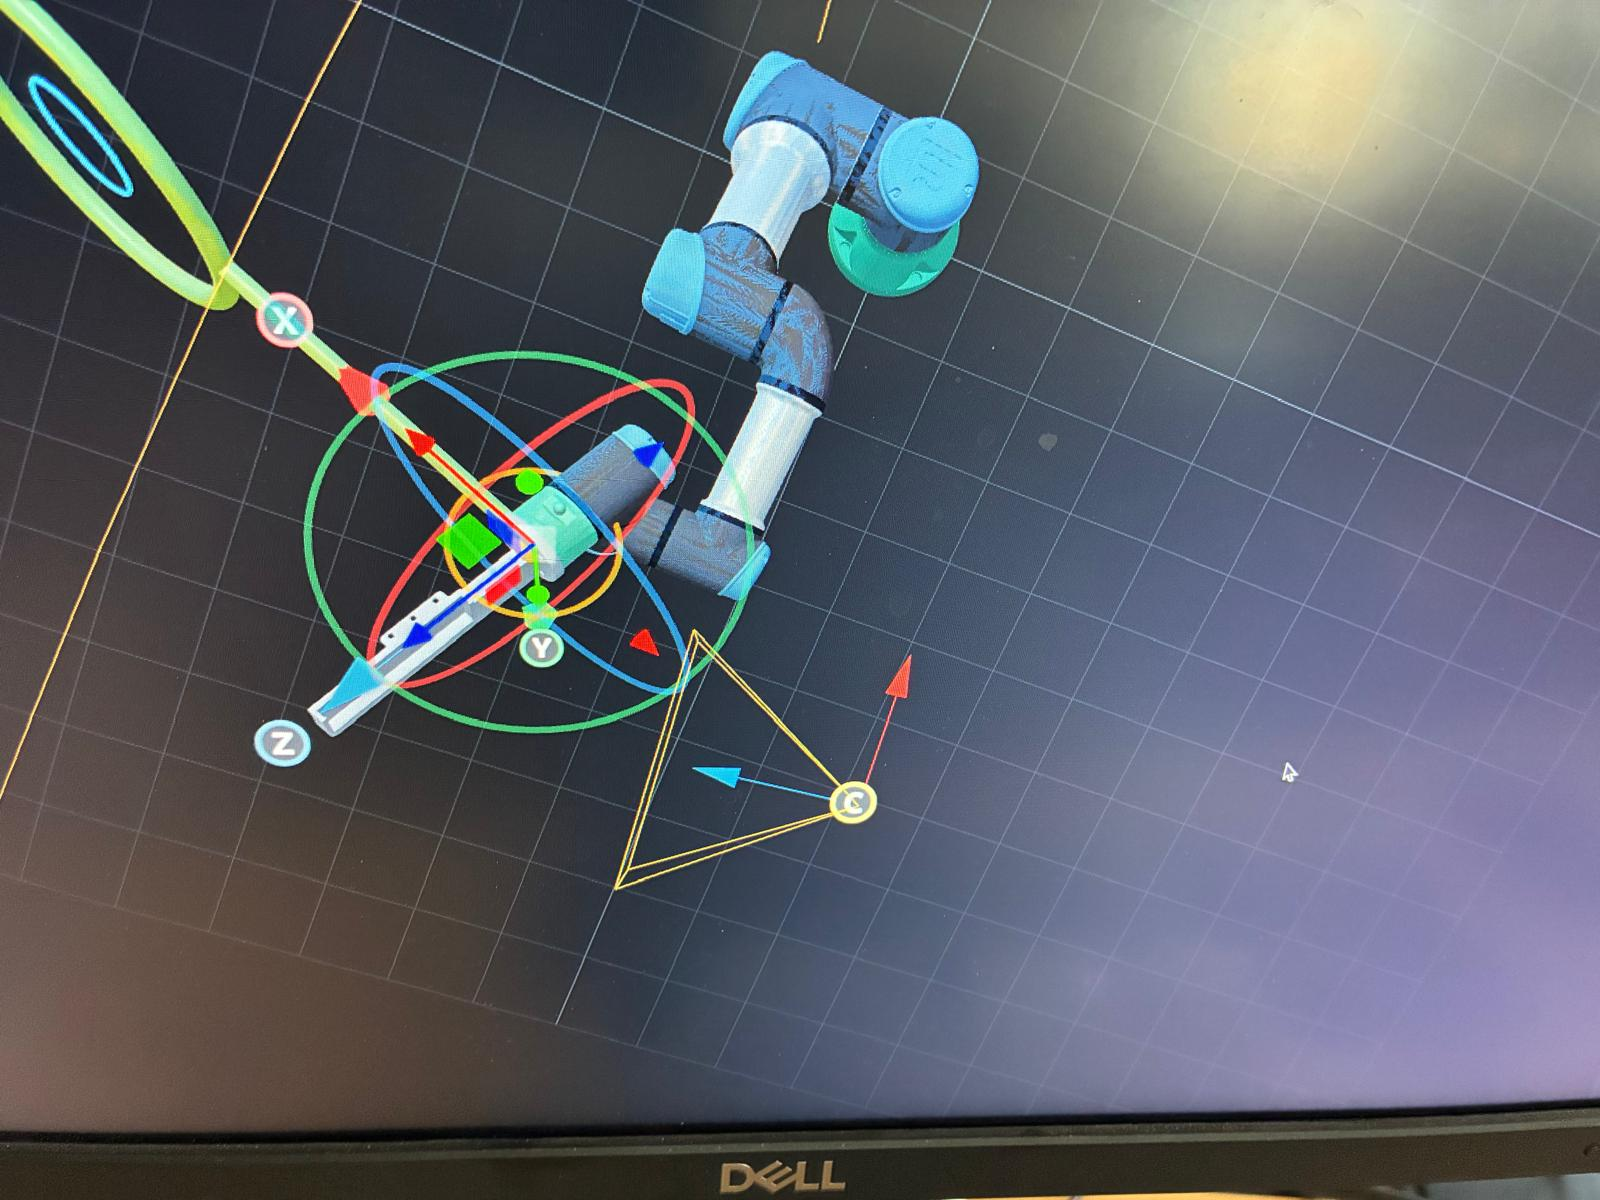
\includegraphics[width=\linewidth]{images/Calibration/Sortie_calibration_extrinseque_1.jpg}
  \end{minipage}
  \hfill
  \begin{minipage}{0.48\textwidth}
    \centering
    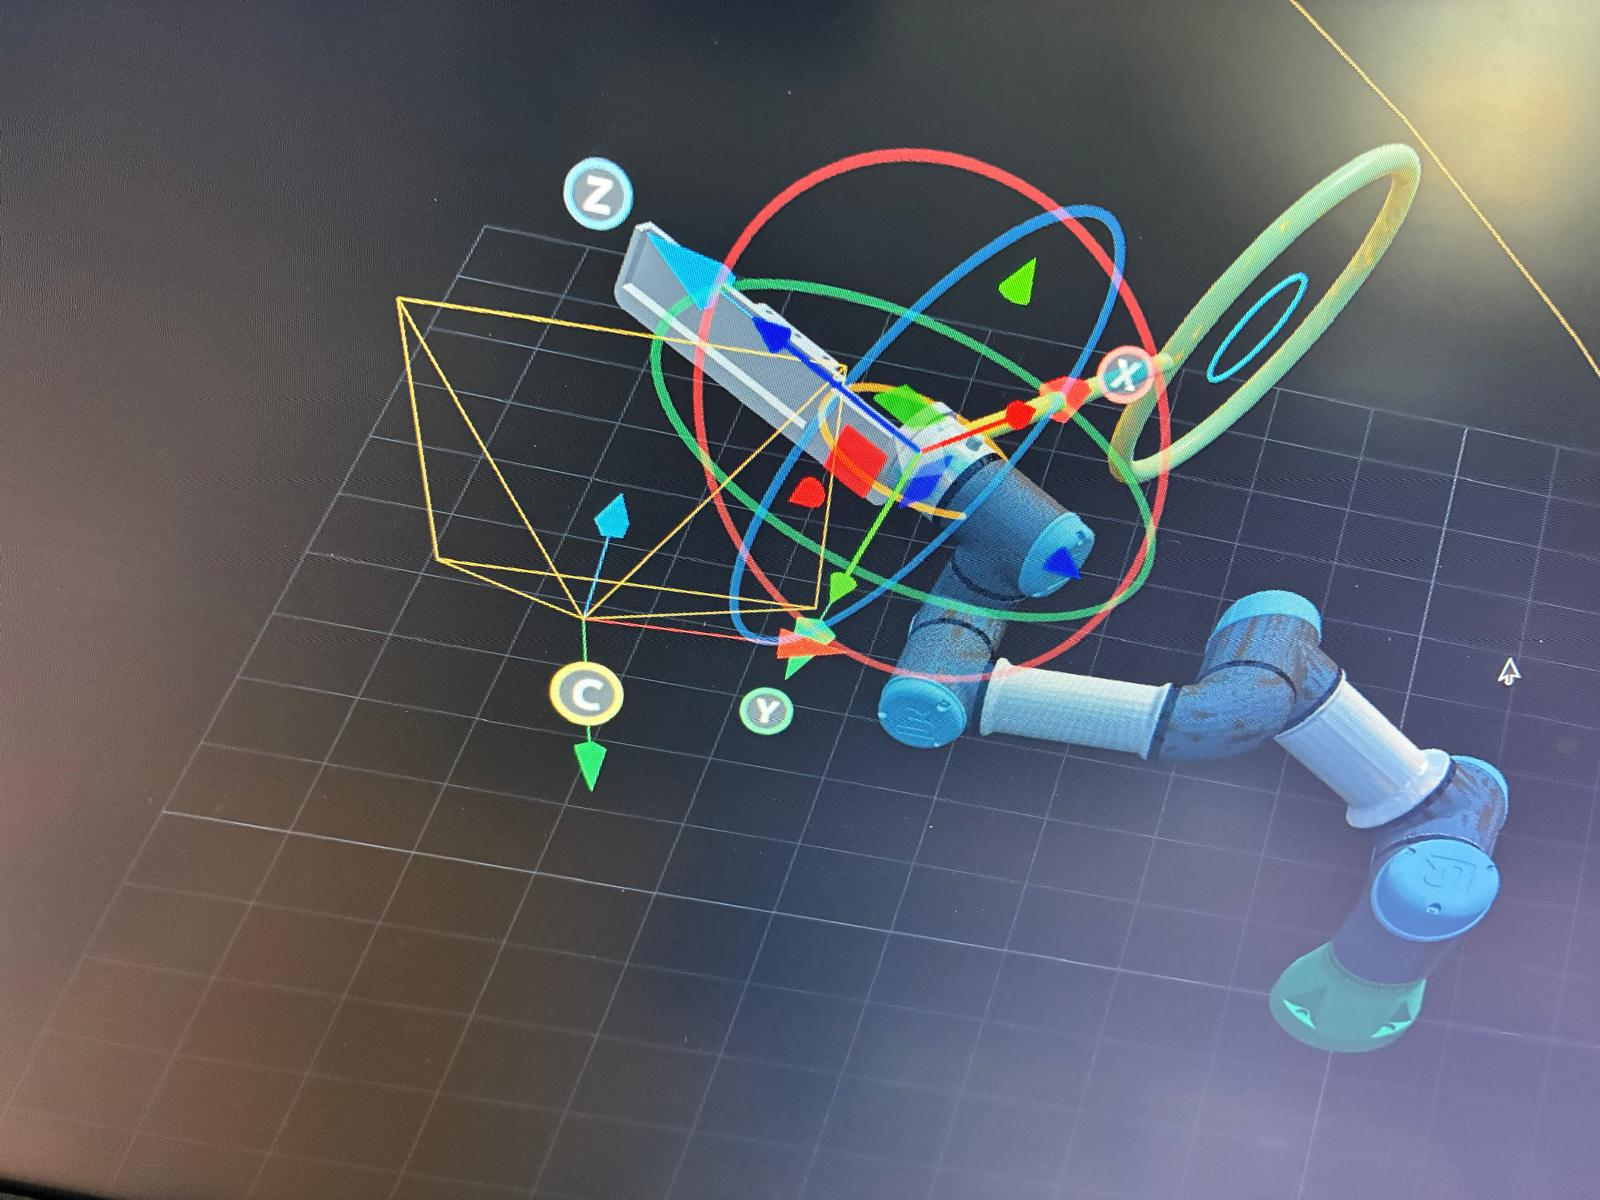
\includegraphics[width=\linewidth]{images/Calibration/Sortie_calibration_extrinseque_2.jpg}
  \end{minipage}
  \caption{Pose 3D de la caméra restituée dans l'interface de supervision après la calibration extrinsèque, sous deux angles de vue. La pyramide jaune représente le champ de vision de la caméra avec son repère; sa position et son orientation par rapport au robot et à l'écran porté par l'effecteur sont cohérentes avec le montage physique de la \figref{fig:handeye-setup-reel}.}
  \label{fig:handeye-ui-3d}
\end{figure}

Cette transformation reste propre à l'installation. Une mesure indépendante du
montage et une vérification de la transformation publiée restent utiles pour
séparer une éventuelle erreur de calibration des autres erreurs de la chaîne.

\subsection{Lien avec l'interception robotique}

Cette calibration est l'étape qui rend la perception exploitable par le robot. Une fois \({}^{B}T_C\) connue, une position de balle estimée dans le repère caméra peut être transformée dans le repère de la base:

\begin{equation}
P^B = {}^{B}T_C\,P^C.
\label{eq:changement-repere-balle}
\end{equation}

Grâce à~\eqref{eq:changement-repere-balle}, la trajectoire obtenue par la méthode Trace peut alors être exprimée dans le repère robot, filtrée, prédite, puis transmise à la commande ou à une politique d'interception. La qualité de cette transformation conditionne directement la précision finale, car même une bonne estimation caméra ne suffit pas si la calibration extrinsèque déplace la balle de plusieurs centimètres dans le repère du robot.

\section{Apprentissage d'une politique d'interception en simulation}

\subsection{Objectif de la partie robot}

La perception doit être associée à une commande capable de déplacer le filet.
Cette partie a été étudiée dans Isaac Lab \cite{nvidia-isaac-lab} avec
l'algorithme d'apprentissage par renforcement PPO
\cite{schulman-ppo}. La simulation permet de répéter les lancers sans risque
pour le robot réel.

\begin{figure}[H]
  \centering
  \includegraphics[page=12,width=0.70\textwidth]{RigonPresentation.pdf}
  \caption{Montage réel visé pour l'interception: robot, caméra et zone de réception.}
  \label{fig:robot-setup}
\end{figure}

\subsection{Environnement d'apprentissage}

L'observation contient \(33\) valeurs décrivant l'état articulaire du robot, la
position du filet, la position et la vitesse de la balle, leur position relative
et la dernière action. La politique produit six actions normalisées,
interprétées à \(60~\text{Hz}\) comme des incréments articulaires limités en
vitesse, en accélération et en position.

Les informations fournies à la politique peuvent être regroupées en trois
familles, présentées dans le tableau~\ref{tab:observation-ppo}. Cette séparation
permet de vérifier que la politique reçoit à la fois l'état du robot, la
géométrie instantanée de l'interception et une mémoire minimale du cycle
précédent. Toutes les positions utilisées pour l'apprentissage sont exprimées
dans un repère équivalent à la base du robot, afin de pouvoir reconstruire la
même observation lors du transfert réel.

\begin{table}[H]
  \centering
  \caption{Structure fonctionnelle de l'observation fournie à la politique PPO.}
  \label{tab:observation-ppo}
  \small
  \begin{tabular}{L{0.25\textwidth}cL{0.57\textwidth}}
    \toprule
    Famille & Dimension & Rôle \\
    \midrule
    État du robot & 12 & Positions et vitesses des six articulations, nécessaires pour produire une action compatible avec la configuration courante. \\
    Balle et filet & 13 & Positions, vitesse de la balle, direction et distance relatives pour décrire la géométrie de l'interception. \\
    Mémoire courte & 8 & Action précédente et indicateurs de passage de la balle, afin de conserver la continuité d'un cycle au suivant. \\
    \bottomrule
  \end{tabular}
\end{table}

Une action ne représente pas directement une position absolue des
articulations. Elle définit un déplacement élémentaire à partir de la consigne
précédente. Avant l'intégration, cette action est bornée, puis la vitesse et
l'accélération articulaires sont limitées. Cette sémantique incrémentale réduit
les discontinuités de consigne et peut être reproduite à l'identique dans la
boucle réelle. Elle laisse néanmoins à la politique la responsabilité de choisir
la direction du mouvement et de coordonner les six articulations.

La récompense favorise la proximité entre la balle et le filet, accorde un bonus
au passage de la balle et pénalise les échecs ainsi que les commandes trop
brusques. Du bruit et un retard sont ajoutés aux observations pour préparer le
transfert réel. Les équations, coefficients et hyperparamètres sont regroupés
dans l'annexe~\ref{ann:env-apprentissage}.

La récompense combine ainsi un signal progressif et un objectif final. Le terme
de proximité guide l'apprentissage avant même qu'une interception ne soit
réussie, tandis que le bonus de passage distingue une trajectoire qui traverse
réellement le plan du filet d'un simple rapprochement. La pénalisation des
actions évite enfin d'obtenir une politique efficace uniquement au prix de
mouvements très brusques. Le bruit et le retard introduits pendant
l'apprentissage cherchent à éviter une dépendance excessive à des observations
parfaites, qui ne seraient pas disponibles avec la caméra réelle.

\subsection{Déroulement et résultats de l'entraînement}

Deux politiques ont été entraînées, une pour chaque côté de montage du filet.
La \figref{fig:ppo-recompense} montre une progression rapide au début, puis une
amélioration plus lente jusqu'à environ \(15\,000\) étapes de collecte. La
récompense moyenne atteint alors environ \(1\,450\) pour la variante droite et
\(1\,600\) pour la variante gauche.

\begin{figure}[H]
  \centering
  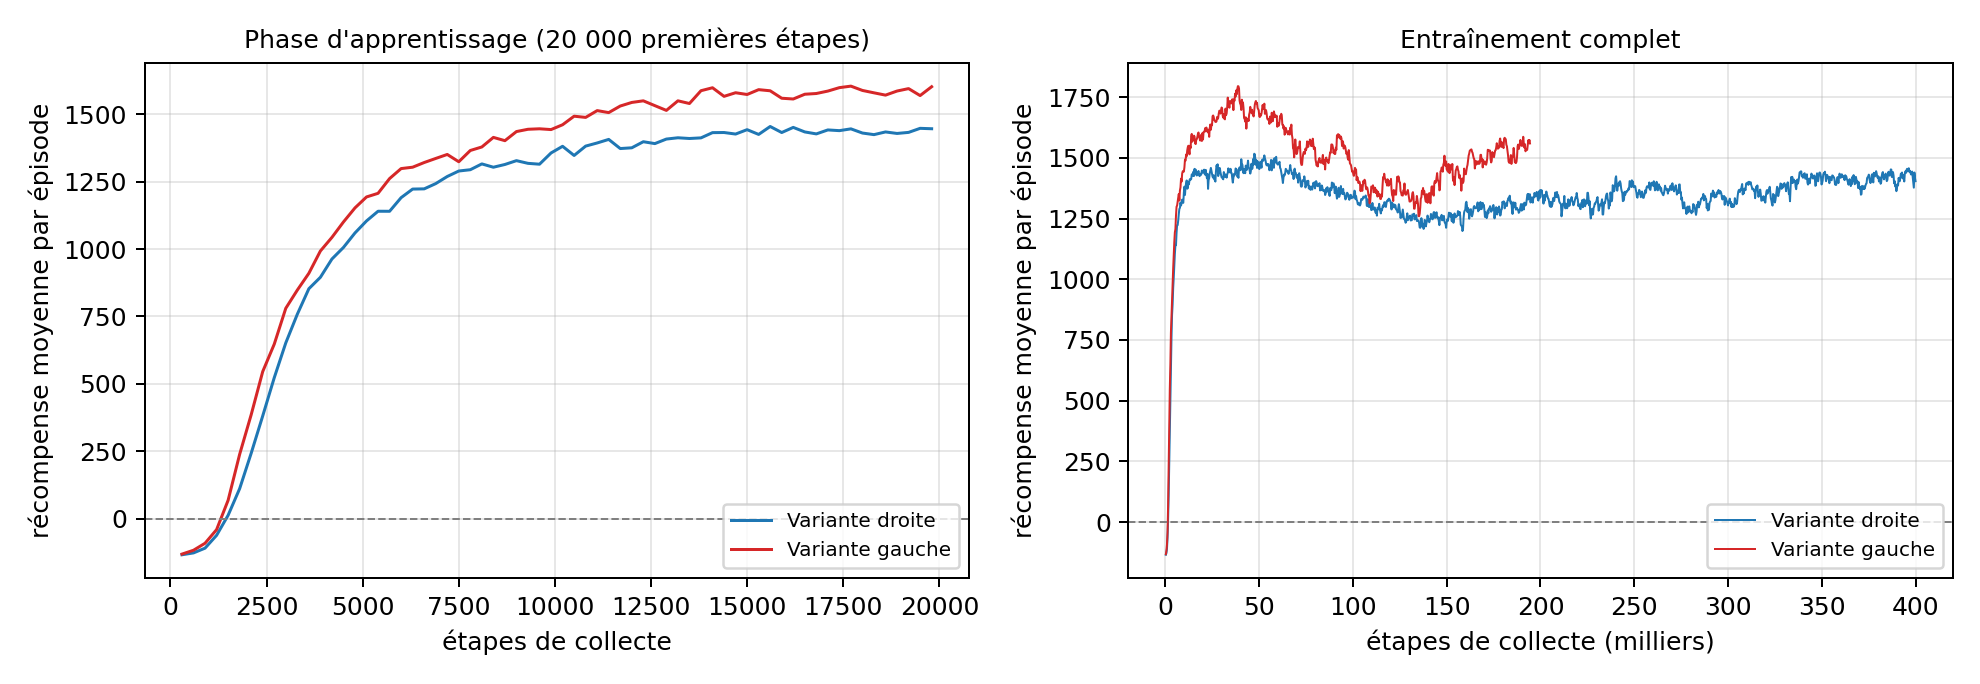
\includegraphics[width=\textwidth]{images/Apprentissage/courbe_recompense_ppo.png}
  \caption{Récompense moyenne au cours des deux entraînements PPO. À gauche, les \(20\,000\) premières étapes; à droite, les entraînements complets. Ces courbes décrivent l'entraînement, et non l'inférence de la politique finale.}
  \label{fig:ppo-recompense}
\end{figure}

Après cette progression, les courbes fluctuent autour d'un niveau stable.
L'entraînement exploitant \(12\,000\) environnements simulés en parallèle,
l'essentiel du comportement est acquis en quelques minutes de calcul et les
heures suivantes ne servent qu'à vérifier cette stabilité: la variante droite a
été poursuivie jusqu'à \(400\,000\) étapes de collecte en \(2\,\text{h}\,45\),
la variante gauche arrêtée à \(194\,000\) étapes en \(1\,\text{h}\,20\). C'est
le dernier état sauvegardé de cette dernière, qui correspond au montage
physique du filet, qui est déployé dans la boucle d'interception.

La récompense moyenne ne doit pas être confondue avec un taux de réussite. Elle
additionne la proximité, le passage dans le filet, les pénalités d'action et les
échecs sur l'ensemble des environnements simulés. Son augmentation montre que
la politique améliore simultanément ces comportements, mais la validation
décisive reste l'exécution sur le robot. Les deux entraînements atteignent des
niveaux différents, car le montage du filet et l'enveloppe des lancers sont
miroités d'un côté à l'autre; une politique est donc associée au côté physique
pour lequel elle a été entraînée.

\section{Boucle d'interception temps réel}

\subsection{Transfert de la politique}

Pour utiliser la politique sur le robot réel, une boucle de commande à \(60~\text{Hz}\) a été mise en place. À chaque cycle, elle reçoit la dernière position de balle estimée, la transforme dans le repère de la base du robot grâce à la calibration extrinsèque, construit le vecteur d'observation de \(33\) valeurs décrit précédemment, exécute la politique apprise, convertit l'action en consigne articulaire avec les mêmes limites de vitesse et d'accélération qu'en simulation, puis applique une couche de sécurité indépendante avant toute transmission au robot. La consigne finale est envoyée au contrôleur du robot sous forme d'un flux interpolé à \(500~\text{Hz}\), ce qui lisse le mouvement entre deux décisions de la politique.

Le transfert ne consiste donc pas uniquement à charger le modèle appris. Trois
conventions doivent rester identiques entre simulation et réalité: l'ordre et
les unités des \(33\) observations, le repère dans lequel la balle et le filet
sont exprimés, et l'interprétation incrémentale des six actions. Une erreur sur
l'une de ces conventions peut produire une commande plausible numériquement,
mais sans rapport avec le comportement appris.

Un cycle de décision peut être résumé ainsi:
\begin{enumerate}
  \item vérifier la fraîcheur de la position de balle et la transformer dans le
  repère de base;
  \item associer cette mesure à l'état articulaire et à la position actuelle du
  filet pour reconstruire l'observation;
  \item calculer l'action de la politique, puis appliquer les limites
  articulaires et les vérifications de sécurité;
  \item interpoler la consigne jusqu'au cycle de décision suivant.
\end{enumerate}

La politique ne reçoit pas un point d'intersection calculé à l'avance. Elle
observe l'évolution de la balle et du filet, puis produit une nouvelle action à
chaque cycle. Le point de rencontre résulte donc du comportement appris en
boucle fermée.

\subsection{Couche de sécurité}

La sécurité est traitée comme une propriété du système et non de la politique. L'émission de commande vers le robot est désactivée par défaut et doit être armée explicitement par l'opérateur. La boucle refuse de commander le robot si aucun modèle de politique n'est chargé, si la position de la balle arrive dans un repère inconnu, ou si la transformation donnant la position du filet n'est pas disponible. Un facteur global de réduction de vitesse permet une montée en régime progressive lors des essais, et un chien de garde interrompt la commande si les données nécessaires cessent d'arriver.

Cette séparation permet de tester la perception et l'inférence sans mouvement,
puis d'autoriser progressivement la commande. Elle protège également le robot
contre une sortie inattendue de la politique: une action reste soumise aux
limites de position, de vitesse et d'accélération avant d'atteindre le
contrôleur. Le fonctionnement sûr ne repose donc pas sur le seul fait que les
trajectoires d'apprentissage étaient valides en simulation.

\section{Premiers essais sur le robot réel}

\subsection{Validation de la chaîne de commande avec une balle virtuelle}

La chaîne de commande a d'abord été validée sans caméra, en remplaçant la perception par un générateur de balles virtuelles suivant la même enveloppe de lancers que la simulation d'apprentissage. Dans cette configuration, la chaîne complète fonctionne sur le robot réel. La politique calcule les actions à partir de la balle virtuelle et le robot amène le filet à sa rencontre, sans qu'aucun point d'intersection ne lui soit fourni: la commande reste une suite d'incréments articulaires produits à chaque cycle à partir de la position courante de la balle. Une fois la balle au sol, le robot maintient sa position. Sous les limites de mise en service, avec le facteur de vitesse réduit de moitié, la réponse du robot reste cependant plus lente que le comportement simulé; l'optimisation de cette réponse fait partie des travaux restants.

Cette étape intermédiaire isole la partie commande. Puisque la trajectoire de la
balle est connue et déjà exprimée dans le bon repère, un échec ne peut pas être
attribué à la détection événementielle ou à la calibration caméra-robot. Elle a
ainsi permis de vérifier le format des observations, le sens des actions et le
comportement des sécurités avant d'ajouter l'incertitude de la perception
réelle.

\subsection{Interception d'une balle réelle}
\label{sec:essais-interception}

La chaîne complète a ensuite été essayée dans sa configuration finale, avec la caméra événementielle réelle, perception par la méthode Trace, politique d'interception et commande du robot activée, avec une balle lancée à la main vers le robot. Le filet est solidarisé au poignet du robot par un support conçu et imprimé en 3D pendant le stage, décrit dans l'annexe~\ref{ann:support-filet}. Dans cette configuration, le robot intercepte effectivement la balle et la retient dans le filet, comme le montre la \figref{fig:interception-reelle}. C'est le premier résultat de bout en bout du projet, et il valide simultanément la perception événementielle, la calibration caméra-robot, la politique apprise en simulation et la boucle de commande temps réel.

\begin{figure}[H]
  \centering
  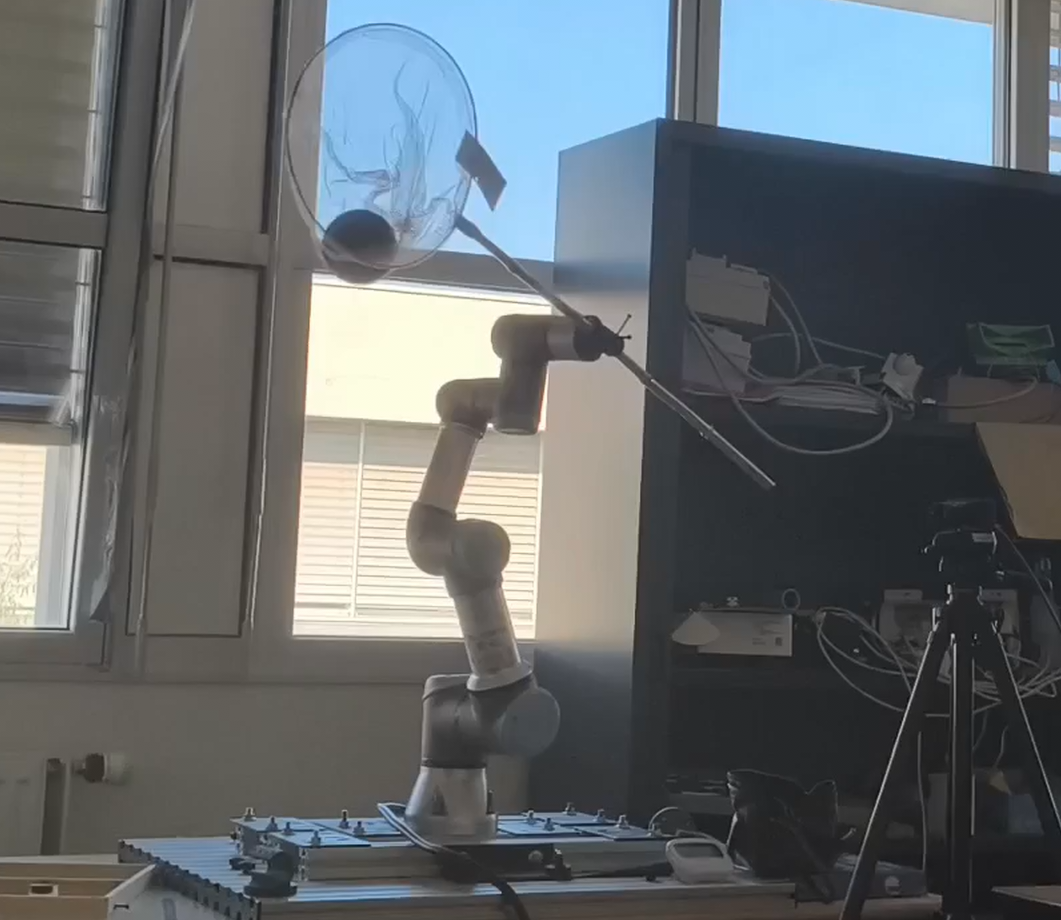
\includegraphics[width=0.58\textwidth]{images/Essais_Reels/interception_balle_reelle.png}
  \caption{Interception réussie d'une balle réelle par le UR3e. La balle est retenue dans le filet porté par l'effecteur, à partir de la seule perception événementielle.}
  \label{fig:interception-reelle}
\end{figure}

La réussite reste toutefois intermittente, environ un lancer sur cinq étant intercepté. Deux causes se dégagent des essais, sans qu'elles aient encore été quantifiées. La première est la latence de la chaîne, entre l'acquisition des événements et le mouvement effectif du robot. Le filet arrive au point d'interception avec un retard qui suffit à manquer une balle rapide. La seconde est un décalage spatial apparent entre la position visée et la position réelle de la balle, dont l'origine reste à déterminer entre un biais résiduel de la perception, une erreur résiduelle de calibration extrinsèque et l'écart entre la dynamique simulée et la dynamique réelle du robot.

L'essai réel ajoute simultanément ces différentes sources d'erreur, ce qui
explique qu'une réussite de bout en bout ne suffise pas à identifier le facteur
limitant. La comparaison avec la balle virtuelle indique néanmoins que la
chaîne de commande et la politique peuvent produire le mouvement attendu. Le
diagnostic doit maintenant porter sur l'âge réel de la mesure au moment où la
commande est exécutée et sur la cohérence spatiale entre la trajectoire
reconstruite et la position physique du filet.

Ces deux points font partie des travaux immédiatement à venir. Le taux de réussite obtenu doit donc être lu comme une première démonstration de faisabilité de la chaîne complète, et non comme une performance d'interception consolidée.

\section{Défis pour l'intégration perception-robot}

Plusieurs difficultés identifiées au début du projet pour passer d'une perception fonctionnelle à une interception fiable ont maintenant une réponse. La calibration caméra-robot est réalisée et validée numériquement, la perception 3D atteint une exactitude compatible avec la taille du filet, la chaîne de commande fonctionne sur le robot réel et les mécanismes de sécurité ont été éprouvés pendant les essais.

Les essais permettent aussi de distinguer les principales sources d'écart qui
se cumulent entre la mesure et l'interception. Le
tableau~\ref{tab:erreurs-bout-en-bout} les relie aux validations réalisées. Il
ne constitue pas un budget d'erreur chiffré, car certaines contributions n'ont
pas encore été mesurées indépendamment, mais il indique quelle expérience
permet de les isoler.

\begin{table}[H]
  \centering
  \caption{Lecture des principales sources d'erreur de la chaîne complète.}
  \label{tab:erreurs-bout-en-bout}
  \small
  \begin{tabular}{L{0.22\textwidth}L{0.31\textwidth}L{0.37\textwidth}}
    \toprule
    Source & Effet attendu & Élément de diagnostic \\
    \midrule
    Largeur apparente & Biais surtout visible sur la profondeur & Comparaison Trace/cercle et ablation de la correction sur vérité terrain. \\
    Calibration & Décalage spatial cohérent d'un lancer à l'autre & Cible carrée indépendante, reprojection multi-poses et validation croisée. \\
    Latence & Filet en retard le long de la trajectoire & Horodatage de la mesure, de la décision et du mouvement effectif. \\
    Dynamique réelle & Mouvement plus lent ou différent de la simulation & Essais avec balle virtuelle, sans erreur de perception. \\
    \bottomrule
  \end{tabular}
\end{table}

Ces contributions ne se manifestent pas de la même manière. Un défaut de
calibration déplace de façon systématique la trajectoire exprimée dans le repère
du robot. Une erreur de largeur varie davantage avec la distance et la densité
d'événements. La latence produit enfin un décalage qui augmente avec la vitesse
de la balle et du robot. Cette distinction est utile pour la suite: corriger un
décalage temporel par une translation fixe, ou inversement compenser une erreur
géométrique par une anticipation, pourrait améliorer quelques lancers tout en
dégrader d'autres.

Les points encore ouverts sont ceux que les essais réels ont fait apparaître, décrits à la section~\ref{sec:essais-interception}, la latence de bout en bout, qu'il faut instrumenter avant de pouvoir la réduire, et le décalage spatial résiduel, dont il reste à séparer les trois contributions possibles. S'y ajoute l'espace atteignable, puisque toutes les trajectoires de balle ne sont pas interceptables dans les limites articulaires et de vitesse du UR3e.

La priorité est donc de mesurer séparément le temps écoulé entre les derniers
événements utilisés, la publication de la position, la décision de la politique
et le mouvement du robot. Une fois la composante temporelle connue, un contrôle
géométrique de la position du filet et de quelques points dans le volume de
travail permettra d'estimer la part restante du décalage spatial. Cette démarche
prolonge la validation par niveaux utilisée pendant le stage et évite de régler
la politique pour masquer une erreur située en amont.

\section{Bilan par rapport au cahier des charges}

Le tableau~\ref{tab:bilan-cahier-charges} reprend les exigences définies au
chapitre~\ref{chap:poste-cadrage}. Il distingue les fonctions effectivement
démontrées des performances qui restent à consolider par davantage d'essais
réels.

\begin{table}[H]
  \centering
  \caption{État des exigences à l'issue du stage.}
  \label{tab:bilan-cahier-charges}
  \small
  \begin{tabular}{L{0.13\textwidth}L{0.18\textwidth}L{0.59\textwidth}}
    \toprule
    Exigences & État & Résultat \\
    \midrule
    F1, P1, P2 & Démontrées en simulation & Position 3D obtenue sur une part majoritaire du vol, avec une erreur nominale de \(4{,}5~\text{cm}\). \\
    F2, P4 & Réalisées & Transformation caméra-base estimée et stable en validation croisée; un contrôle physique indépendant reste souhaitable. \\
    F3, P3 & Atteintes & Estimation Trace en \(1{,}7~\text{ms}\) en moyenne et boucle de décision exécutée à \(60~\text{Hz}\). \\
    F4 & Démontrée & Une balle réelle a été interceptée, mais la réussite reste intermittente. \\
    F5 & Réalisée & Commande désarmée par défaut, limites articulaires et arrêt en cas de données manquantes. \\
    \bottomrule
  \end{tabular}
\end{table}

Le système remplit ainsi les fonctions nécessaires à une démonstration de bout
en bout. La différence entre une démonstration et une performance consolidée se
situe principalement dans la répétabilité de l'interception réelle, aujourd'hui
limitée par la latence et le décalage spatial décrits précédemment.

\chapter{Conclusion}

\section*{Bilan technique}

\begin{table}[H]
  \centering
  \caption{Récapitulatif synthétique des réalisations du stage et de l'état atteint.}
  \label{tab:bilan-realisations}
  \scriptsize
  \begin{tabular}{L{0.32\textwidth}L{0.60\textwidth}}
    \toprule
    Thème & Réalisations et état atteint \\
    \midrule
    Perception & Deux méthodes 3D développées et comparées à une vérité terrain. La méthode Trace atteint \(0{,}045~\text{m}\) d'erreur 3D en régime nominal, environ trois fois moins que l'ajustement de cercle. \\
    Calibration & Mire événementielle intrinsèque à \(0{,}149~\text{px}\) RMS et calibration caméra-robot à \(1{,}11~\text{mm}\) et \(0{,}27^\circ\) de résidu moyen. Une vérification physique indépendante reste souhaitable. \\
    Apprentissage et commande & Politique PPO apprise en simulation, boucle de décision à \(60~\text{Hz}\), consignes interpolées à \(500~\text{Hz}\) et mécanismes de sécurité pour les essais réels. \\
    Résultat final & Interception et maintien d'une balle réelle dans le filet. La réussite reste intermittente, environ un lancer sur cinq, principalement à cause de la latence et d'un décalage spatial encore à quantifier. \\
    \bottomrule
  \end{tabular}
\end{table}

L'objectif central du stage, produire une position 3D exploitable d'une balle
rapide et l'utiliser pour une interception robotique, a donc été atteint. La
démonstration réelle confirme la faisabilité de la chaîne complète, sans encore
constituer une performance stabilisée. La suite du projet devra surtout réduire
la latence et identifier l'origine du décalage spatial observé.

\section*{Bilan personnel}

Ce stage m'a permis de travailler sur un système mécatronique complet, du
capteur jusqu'au mouvement du robot, dans un contexte de recherche appliquée.
J'y ai appris à raisonner sur des compromis concrets, fenêtre temporelle contre
réactivité, robustesse contre latence, généralité contre performance temps réel,
et à ne conclure qu'à partir d'une mesure: c'est la comparaison contre une
vérité terrain, et non l'impression visuelle laissée par une trajectoire, qui a
permis de départager les deux méthodes de perception. Les essais sur le robot
réel ont été les plus formateurs. Ils m'ont montré que la mise en service d'un
système robotique repose autant sur la rigueur des procédures et sur la
discipline de l'architecture, en particulier une sécurité traitée indépendamment
de la politique apprise, que sur les algorithmes eux-mêmes. Enfin, les points
réguliers avec mes encadrants m'ont appris à présenter des résultats
intermédiaires, à en assumer les limites et à réorienter le travail en fonction
de ce qu'ils montraient, ce qui est précisément ce qui a conduit à abandonner
l'ajustement de cercle au profit de la méthode par trace.

\appendix

\chapter{Expressions des régressions de trajectoire par moindres carrés}
\label{ann:regressions}

Cette annexe détaille les expressions utilisées pour ajuster les modèles de trajectoire présentés dans la partie perception. Les coordonnées horizontales sont modélisées par une droite et la coordonnée verticale par une parabole; les coefficients sont calculés directement à partir de sommes accumulées au fil des mesures, sans résolution matricielle générale.

Pour une coordonnée linéaire \(q \in \{X,Y\}\), avec \(n\) observations \((t_i, q_i)\):

\begin{equation}
D = n \sum t_i^2 - \left(\sum t_i\right)^2,
\label{eq:mc-denominateur}
\end{equation}

\begin{equation}
a = \frac{n \sum t_i q_i - \left(\sum t_i\right)\left(\sum q_i\right)}{D},
\qquad
b = \frac{\sum q_i - a \sum t_i}{n}.
\label{eq:mc-lineaire}
\end{equation}

Pour la coordonnée quadratique \(Z\), le modèle est \(q(t) = a t^2 + b t + c\). Les grandeurs intermédiaires utilisées sont:

\begin{equation}
S_{11} = \sum t_i^2 - \frac{\left(\sum t_i\right)^2}{n},
\qquad
S_{12} = \sum t_i^3 - \frac{\left(\sum t_i\right)\left(\sum t_i^2\right)}{n},
\label{eq:mc-quad-a}
\end{equation}

\begin{equation}
S_{22} = \sum t_i^4 - \frac{\left(\sum t_i^2\right)^2}{n},
\qquad
S_{q1} = \sum t_i q_i - \frac{\left(\sum q_i\right)\left(\sum t_i\right)}{n},
\label{eq:mc-quad-b}
\end{equation}

\begin{equation}
S_{q2} = \sum t_i^2 q_i - \frac{\left(\sum q_i\right)\left(\sum t_i^2\right)}{n},
\qquad
D_q = S_{22}S_{11} - S_{12}^2.
\label{eq:mc-quad-c}
\end{equation}

Les coefficients quadratiques sont alors:

\begin{equation}
b = \frac{S_{q1}S_{22} - S_{q2}S_{12}}{D_q},
\qquad
a = \frac{S_{q2}S_{11} - S_{q1}S_{12}}{D_q},
\qquad
c = \bar{q} - b\bar{t} - a\overline{t^2}.
\label{eq:mc-quad-coeffs}
\end{equation}

La version pondérée conserve les mêmes modèles mais remplace chaque somme simple par la somme pondérée correspondante. Le poids d'un point combine un terme de récence et un terme robuste fondé sur le résidu:

\begin{equation}
w_i =
\exp\left(-3\,\frac{t_{\max}-t_i}{t_{\max}-t_{\min}}\right)
\cdot
\frac{1}{1+\left(\frac{r_i}{s}\right)^2},
\label{eq:poids-regression}
\end{equation}

où \(r_i\) est le résidu par rapport à la première régression et \(s\) une échelle robuste calculée à partir de la médiane des résidus. Les points récents et cohérents ont donc plus d'influence que les points anciens ou aberrants. Cette pondération est commune aux deux méthodes de perception.

\chapter{Pipeline détaillé de la détection par circle fitting}
\label{ann:pipeline-circle}

Cette annexe détaille les étapes internes de la méthode par circle fitting, dont la vue simplifiée est donnée par la \figref{fig:algo-fitting-circle}. La \figref{fig:pipeline-circle-detaille} décompose les trois phases du traitement, la réduction du flux d'événements, la validation du cluster avec l'ajustement du cercle, puis le calcul de la pose 3D et de la trajectoire.

\begin{figure}[H]
  \centering
  \resizebox{\textwidth}{!}{%
  \begin{tikzpicture}[
      font=\small,
      block/.style={draw, rounded corners=2pt, align=center, text width=2.6cm, minimum height=1.35cm},
      source/.style={block, fill=blue!8},
      prep/.style={block, fill=cyan!8},
      clust/.style={block, fill=orange!12},
      fitc/.style={block, fill=violet!10},
      valid/.style={block, fill=red!8},
      output/.style={block, fill=green!10},
      phase/.style={font=\small\bfseries},
      note/.style={draw, rounded corners=2pt, align=center, fill=red!5, font=\footnotesize},
      arrow/.style={-{Latex[length=2.5mm]}, thick},
      lbl/.style={font=\scriptsize\itshape, align=center}
    ]
    % Phase 1
    \node[phase] at (9.3,1.35) {Phase 1: prétraitement et réduction du flux};
    \node[source] (acq)    at (0,0)    {Acquisition\\caméra ou séquence enregistrée};
    \node[prep]   (noise)  at (3.1,0)  {Filtre à bruit\\activité isolée supprimée};
    \node[prep]   (recent) at (6.2,0)  {Fenêtre récente\\événements des derniers instants};
    \node[prep]   (ech)    at (9.3,0)  {Échantillonnage\\limitation du nombre de points};
    \node[prep]   (undist) at (12.4,0) {Correction de distorsion\\modèle intrinsèque calibré};
    \node[prep]   (roi)    at (15.5,0) {Zone d'intérêt\\restriction spatiale et temporelle};
    \node[clust]  (dbscan) at (18.6,0) {Regroupement DBSCAN\\clusters 2D triés par taille};

    \draw[arrow] (acq) -- (noise);
    \draw[arrow] (noise) -- (recent);
    \draw[arrow] (recent) -- (ech);
    \draw[arrow] (ech) -- (undist);
    \draw[arrow] (undist) -- (roi);
    \draw[arrow] (roi) -- (dbscan);

    % Phase 2
    \node[phase] at (9.3,-1.85) {Phase 2: validation du cluster et ajustement du cercle};
    \node[clust] (cand)   at (0,-3.2)    {Cluster candidat\\points, polarités,\\durée};
    \node[fitc]  (slice)  at (3.1,-3.2)  {Sous-tranche optionnelle\\par temps ou par nombre};
    \node[fitc]  (fit1)   at (6.2,-3.2)  {Premier cercle\\moindres carrés sur le contour};
    \node[valid] (polar)  at (9.3,-3.2)  {Validation des polarités\\symétrie des directions};
    \node[valid] (outl)   at (12.4,-3.2) {Rejet des aberrants\\résidu RMS par point};
    \node[fitc]  (fit2)   at (15.5,-3.2) {Second cercle\\réajustement et contrôle du rayon};
    \node[fitc]  (okc)    at (18.6,-3.2) {Cercle validé\\centre \((u,v)\),\\rayon \(r\)};

    \draw[arrow] (cand) -- (slice);
    \draw[arrow] (slice) -- (fit1);
    \draw[arrow] (fit1) -- (polar);
    \draw[arrow] (polar) -- (outl);
    \draw[arrow] (outl) -- (fit2);
    \draw[arrow] (fit2) -- (okc);

    \node[note, text width=12.4cm] (reject) at (9.3,-5.05)
      {Si une validation échoue: rejet de la sous-tranche ou du cluster, puis essai du candidat suivant.};
    \draw[arrow, dashed, red!60] (polar.south) -- (reject.north -| polar.south);
    \draw[arrow, dashed, red!60] (outl.south) -- (reject.north -| outl.south);
    \draw[arrow, dashed, red!60] (fit2.south) -- (reject.north -| fit2.south);

    % Phase 3
    \node[phase] at (9.3,-6.1) {Phase 3: pose 3D, historique et trajectoire};
    \node[output] (pose)  at (0,-7.7)    {Pose 3D\\projection inverse en millimètres};
    \node[valid]  (jump)  at (3.72,-7.7) {Rejet anti-saut\\variation de profondeur trop rapide};
    \node[output] (hist)  at (7.44,-7.7) {Historique\\positions 3D datées};
    \node[output] (regr)  at (11.16,-7.7){Régression\\\(X,Y\) linéaires,\\\(Z\) quadratique};
    \node[output] (pub)   at (14.88,-7.7){Publication\\position 3D pour la partie robotique};
    \node[output] (disp)  at (18.6,-7.7) {Affichage\\vues 2D et 3D de contrôle};

    \draw[arrow] (pose) -- (jump);
    \draw[arrow] (jump) -- (hist);
    \draw[arrow] (hist) -- (regr);
    \draw[arrow] (regr) -- (pub);
    \draw[arrow] (pub) -- (disp);

    % Inter-phase connectors
    \draw[arrow] (dbscan.south) -- ++(0,-0.5) -| ($(cand.north)+(0,0.5)$) -- (cand.north);
    \draw[arrow] (okc.south) -- ++(0,-2.9) -| ($(pose.north)+(0,0.5)$) -- (pose.north);

    % Formules
    \node[align=center, font=\small] at (9.3,-9.6)
      {\(Z = \dfrac{f_x\,R}{r}\) \qquad
       \(X = \dfrac{(u-c_x)\,Z}{f_x}\) \qquad
       \(Y = \dfrac{(v-c_y)\,Z}{f_y}\) \qquad
       avec \(R\) le rayon réel de la balle.};
  \end{tikzpicture}}
  \caption{Pipeline détaillé de la détection 3D par circle fitting, en trois phases: réduction du flux d'événements, validation du cluster et ajustement du cercle, puis pose 3D et trajectoire. Les formules du bas donnent la conversion du cercle image \((u,v,r)\) en position 3D dans le repère caméra.}
  \label{fig:pipeline-circle-detaille}
\end{figure}

\section*{Expressions de la validation par symétrie des polarités}

La validation décrite dans le corps du rapport repose sur la répartition angulaire des polarités autour du centre du cercle candidat. Pour chaque événement \(p_i\), on calcule le vecteur radial normalisé

\begin{equation}
d_i = \frac{p_i - c}{\|p_i - c\|},
\label{eq:direction-radiale}
\end{equation}

où \(c\) est le centre du cercle estimé. Ces vecteurs sont ensuite séparés selon leur polarité et accumulés:

\begin{equation}
D_+ = \sum_{p_i = +} d_i,
\qquad
D_- = \sum_{p_i = -} d_i.
\label{eq:sommes-polarites}
\end{equation}

L'angle moyen de chaque polarité s'en déduit,

\begin{equation}
\theta_+ = \operatorname{atan2}(D_{+,y}, D_{+,x}),
\qquad
\theta_- = \operatorname{atan2}(D_{-,y}, D_{-,x}),
\label{eq:angles-moyens}
\end{equation}

et la séparation entre ces deux directions doit rester proche de \(\pi\) à une tolérance \(\varepsilon\) près, c'est-à-dire que les deux groupes doivent être approximativement opposés:

\begin{equation}
\left||\theta_+ - \theta_-| - \pi\right| < \varepsilon.
\label{eq:critere-opposition}
\end{equation}

\section*{Diagnostic du biais de profondeur en fonction de la vitesse}

Ce diagnostic, évoqué dans le corps du rapport, cherche à savoir si l'écart au plan de lancer attendu croît avec la vitesse de la balle. La vue de dessus ajuste d'abord une droite \(Y = aX + b\) aux estimations 3D projetées dans le plan \(X/Y\); cette droite représente le plan vertical attendu vu du dessus. Pour chaque estimation \(P_i = (X_i,Y_i,Z_i)\), la distance orthogonale à cette droite vaut

\begin{equation}
d_i =
\frac{|aX_i - Y_i + b|}{\sqrt{a^2 + 1}}.
\label{eq:distance-plan}
\end{equation}

La vitesse de comparaison est celle dans le plan caméra \(X/Z\), obtenue à partir de la régression de trajectoire:

\begin{equation}
v_{XZ}(t) =
\sqrt{a_X^2 + \left(2a_Zt + b_Z\right)^2}.
\label{eq:vitesse-plan-camera}
\end{equation}

La distance \(d_i\) est tracée en fonction de \(v_{XZ}(t_i)\), puis une régression linéaire \(d \approx \alpha v_{XZ} + \beta\) est ajustée. La \figref{fig:circle-fitting-speed-depth-bias} présente cette analyse.

\begin{figure}[H]
  \centering
  
\includegraphics[width=\textwidth]{\detokenize{images/Algo_Cricle_Fitting/Estimation_coef.png}}
  \caption{Analyse du biais de profondeur. En haut à droite, la vue de dessus montre le décalage des estimations par rapport au plan attendu; le graphique adjacent trace la distance orthogonale à ce plan en fonction de la vitesse estimée dans le plan caméra. La tendance linéaire suggère une proportionnalité entre vitesse et erreur de profondeur.}
  \label{fig:circle-fitting-speed-depth-bias}
\end{figure}

\chapter{Détails de la reconstruction du ruban de trace}
\label{ann:trace-details}

Cette annexe détaille les critères et les expressions utilisés par la méthode par trace événementielle pour reconstruire le ruban, dont les étapes principales sont résumées dans la partie perception.

\section*{Repère local de la trace}

Le centre \(c\) du nuage est estimé de manière robuste avec les médianes des coordonnées, puis les points trop éloignés sont retirés à partir d'un quantile radial. Une PCA globale fournit ensuite la direction principale \(d\) de la trace. Pour les trajectoires courbes, cette direction est corrigée par des PCA temporelles calculées sur plusieurs sous-parties de la trace; l'orientation finale combine la direction globale, la moyenne pondérée des directions locales et le déplacement temporel entre le début et la fin de la trace. Le repère local est défini par:

\begin{equation}
s = (p - c) \cdot d,
\qquad
h = (p - c) \cdot n,
\label{eq:repere-trace}
\end{equation}

où \(p\) est un événement image et \(n=(-d_y,d_x)\) est la normale à la trace. Dans les schémas de cette annexe, l'axe \(h\) est dessiné verticalement comme une hauteur; il s'agit en réalité de la coordonnée transversale à la trace, et l'étendue des événements selon \(h\) correspond donc à la largeur locale du ruban, celle mesurée dans chaque bin.

\section*{Bins spatiaux}

La trace est découpée en bins spatiaux le long de \(s\). Chaque bin \(j\) produit une estimation locale unique, composée de trois valeurs:

\begin{equation}
(s_j,h_{\text{bas},j}),
\qquad
(s_j,h_{\text{milieu},j}),
\qquad
(s_j,h_{\text{haut},j}),
\qquad \text{avec} \quad
h_{\text{milieu},j}=\frac{h_{\text{haut},j}+h_{\text{bas},j}}{2}.
\label{eq:bin-estimations}
\end{equation}

La position \(s_j\) du bin est une valeur représentative des coordonnées \(s\) de ses événements, par exemple la médiane, et la largeur locale vaut \(w_j = h_{\text{haut},j}-h_{\text{bas},j}\).

\section*{Détection des bords soutenus}

Prendre directement \(h_{\text{bas}}=\min h_i\) et \(h_{\text{haut}}=\max h_i\) serait trop sensible au bruit, un seul événement isolé devenant un faux bord et faussant la largeur, donc la profondeur. Un bord n'est donc accepté que s'il est soutenu par assez d'événements voisins. Le support requis \(n_{\text{support}}\) est une fraction du nombre d'événements du bin, bornée entre un minimum et un maximum fixés.

Les valeurs de \(h\) sont triées, puis balayées depuis chaque extrémité. Pour le bord bas, le balayage part du plus petit \(h\) et retient le premier candidat \(h_k\) dont la fenêtre \([h_k,\ h_k+r_s]\) contient au moins \(n_{\text{support}}\) événements, où \(r_s\) est le rayon de support, exprimé en pixels et fixé par réglage. Le bord haut est obtenu de manière symétrique, en partant des grandes valeurs de \(h\). La \figref{fig:trace-support-edges} illustre cette logique. Les points isolés aux extrémités ne sont pas retenus comme bords s'ils ne possèdent pas assez de voisins proches.

\begin{figure}[H]
  \centering
  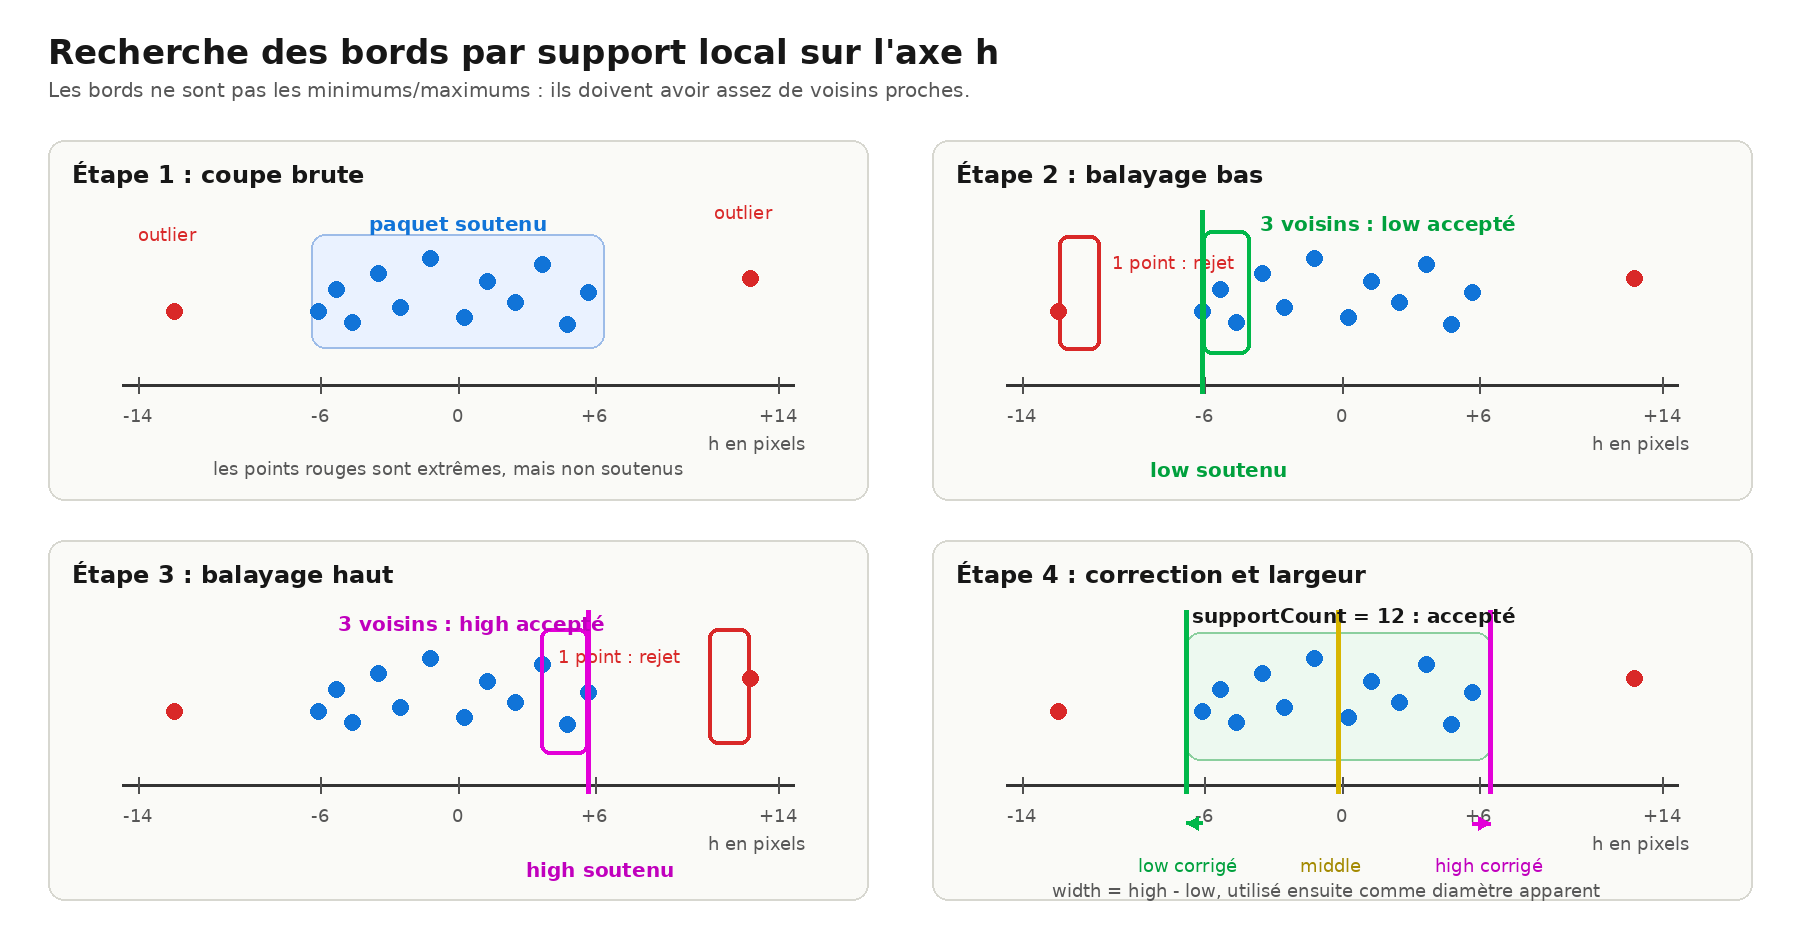
\includegraphics[width=\textwidth]{images/Algo_Trace/Trace_Support_Edges_crop.png}
  \caption{Recherche locale des bords par support sur l'axe \(h\). Les événements isolés sont ignorés; seuls les extrêmes possédant assez de voisins proches deviennent \(h_{\text{bas}}\) et \(h_{\text{haut}}\). L'écart entre ces deux bords, dessiné ici comme une hauteur, est la largeur locale du bin.}
  \label{fig:trace-support-edges}
\end{figure}

Comme les événements correspondent aux centres des pixels, le bord apparent
peut se trouver légèrement au-delà du dernier événement soutenu. La correction
introduite dans~\eqref{eq:correction-largeur-trace} déplace donc chaque bord vers
l'extérieur. Elle comprend une constante \(\delta_{px}=0{,}75~\text{px}\), qui
compense la quantification centre-pixel, et un terme
\(\kappa\bar{s}_{\text{bord}}\) avec \(\kappa=1{,}75\), qui dépend de
l'espacement médian mesuré entre les événements proches du bord. Cette seconde
contribution augmente pour une trace peu dense et devient faible lorsque les
échantillons sont rapprochés. La coupe est enfin validée. Elle est rejetée si
elle contient trop peu d'événements, si
\(h_{\text{haut}}\leq h_{\text{bas}}\), si la largeur brute est trop faible, ou
si le nombre d'événements compris entre les deux bords finaux reste inférieur
au support minimal.

\section*{Filtrage des estimations locales}

Le filtrage se fait en deux niveaux. Le premier vérifie la cohérence globale du ruban. Un modèle polynomial simple, linéaire ou quadratique selon le nombre d'échantillons, est ajusté sur les lignes médianes, et un bin est rejeté si sa ligne médiane est trop éloignée de la tendance générale ou si sa largeur locale est trop différente de la largeur médiane du ruban.

Le second niveau vérifie la cohérence locale. Pour chaque bin \(j\), une petite régression sur les bins voisins, par exemple \(j-4\) à \(j+4\) en ignorant le bin courant pour éviter qu'il ne se valide lui-même, prédit les valeurs attendues \(\hat{h}_{\text{bas},j}\), \(\hat{h}_{\text{milieu},j}\), \(\hat{h}_{\text{haut},j}\) et \(\hat{w}_j\). Le bin est supprimé s'il casse la continuité locale:

\begin{equation}
\begin{aligned}
|w_j - \hat{w}_j| &> \tau_w,
& |h_{\text{bas},j}-\hat{h}_{\text{bas},j}| &> \tau_{\text{bas}}, \\
|h_{\text{milieu},j}-\hat{h}_{\text{milieu},j}| &> \tau_{\text{milieu}},
& |h_{\text{haut},j}-\hat{h}_{\text{haut},j}| &> \tau_{\text{haut}}.
\end{aligned}
\label{eq:filtrage-local}
\end{equation}

où les seuils \(\tau\) dépendent de la largeur médiane du ruban et de la dispersion locale, estimée par l'écart absolu médian des échantillons voisins. Cette étape évite deux erreurs opposées, garder un bin totalement incohérent qui ferait exploser la largeur, donc la profondeur; ou supprimer un bin simplement parce qu'il s'écarte de la moyenne globale alors qu'il reste cohérent avec son voisinage. La \figref{fig:trace-local-neighbour-filter} résume ce principe.

\begin{figure}[H]
  \centering
  \begin{tikzpicture}[x=1.05cm,y=0.9cm,>=Latex]
    \draw[-Latex,thick] (0,0) -- (9.2,0) node[right] {$s$};
    \draw[-Latex,thick] (0,-0.2) -- (0,3.2) node[above] {$h$};

    \foreach \x/\y in {0.8/0.8,1.6/1.0,2.4/1.15,3.2/1.35,4.0/1.55,4.8/2.85,5.6/1.85,6.4/2.0,7.2/2.15,8.0/2.35}
      \fill[black] (\x,\y) circle (1.8pt);

    \draw[dashed,thick] (0.6,0.75) .. controls (2.5,1.1) and (6.2,1.9) .. (8.2,2.35);
    \draw[red,thick] (4.8,2.85) circle (5pt);
    \node[above] at (4.8,3.05) {bin aberrant};
    \node[below] at (4.8,-0.15) {$j$};
    \draw[decorate,decoration={brace,amplitude=5pt}] (2.4,-0.55) -- (7.2,-0.55)
      node[midway,below=5pt] {voisins utilisés pour prédire le bin $j$};
  \end{tikzpicture}
  \caption{Principe du filtrage local. Le bin courant est comparé à une prédiction construite avec ses voisins; s'il crée une rupture trop forte, il est supprimé.}
  \label{fig:trace-local-neighbour-filter}
\end{figure}

\section*{Courbes du ruban}

Après filtrage, il reste trois listes d'échantillons \(\{(s_j,h_{\text{bas},j})\}\), \(\{(s_j,h_{\text{milieu},j})\}\) et \(\{(s_j,h_{\text{haut},j})\}\). Les trois courbes sont ajustées indépendamment, ce qui laisse le ruban souple, car le bord haut et le bord bas ne sont pas forcés d'avoir exactement la même forme, ce qui est utile si la trace est asymétrique ou si une polarité domine localement.

L'ajustement est local: autour d'une position \(s_0\), les échantillons proches pèsent davantage que les échantillons éloignés. Pour un ajustement local quadratique centré sur \(s_0\):

\begin{equation}
h(s) = a(s-s_0)^2 + b(s-s_0) + c,
\qquad
h(s_0)=c.
\label{eq:fit-local}
\end{equation}

Les coefficients sont recalculés pour plusieurs positions \(s_0\) le long du ruban, et la fenêtre locale peut être élargie dans les zones pauvres en échantillons afin de conserver une estimation stable. Chaque point estimé est ensuite reconverti dans le repère image avec:

\begin{equation}
p(s_0) = c_{\text{trace}} + s_0 d + h(s_0)n,
\label{eq:retour-image}
\end{equation}

où \(c_{\text{trace}}\) est le centre du ruban, \(d\) sa direction principale et \(n\) sa normale. La \figref{fig:trace-local-fit-curves} illustre cet ajustement.

\begin{figure}[H]
  \centering
  \begin{tikzpicture}[x=0.95cm,y=0.8cm,>=Latex]
    \draw[-Latex,thick] (0,0) -- (9,0) node[right] {$s$};
    \draw[-Latex,thick] (0,-1.2) -- (0,3.0) node[above] {$h$};

    \foreach \x/\yb/\ym/\yh in {0.8/0.2/1.0/1.8,1.6/0.35/1.12/1.9,2.4/0.55/1.3/2.05,3.2/0.75/1.45/2.18,4.0/0.9/1.55/2.28,4.8/1.05/1.68/2.42,5.6/1.15/1.82/2.55,6.4/1.35/1.98/2.68,7.2/1.55/2.15/2.8,8.0/1.75/2.35/2.95}
    {
      \fill[magenta] (\x,\yb) circle (1.6pt);
      \fill[orange] (\x,\ym) circle (1.6pt);
      \fill[green!60!black] (\x,\yh) circle (1.6pt);
    }

    \draw[magenta,thick] (0.7,0.15) .. controls (2.7,0.55) and (5.3,1.05) .. (8.2,1.78);
    \draw[orange,thick,dashed] (0.7,0.95) .. controls (2.8,1.35) and (5.4,1.75) .. (8.2,2.35);
    \draw[green!60!black,thick] (0.7,1.78) .. controls (2.8,2.05) and (5.4,2.52) .. (8.2,2.95);

    \node[right] at (8.25,2.95) {$h_{\text{haut}}(s)$};
    \node[right] at (8.25,2.35) {$h_{\text{milieu}}(s)$};
    \node[right] at (8.25,1.78) {$h_{\text{bas}}(s)$};

    \draw[gray,densely dashed] (4.8,-1.05) -- (4.8,3.0);
    \node[above right] at (4.8,0.05) {$s_0$};
    \draw[decorate,decoration={brace,amplitude=5pt}] (3.2,-0.95) -- (6.4,-0.95)
      node[midway,below=8pt] {fenêtre locale de fit};
  \end{tikzpicture}
  \caption{Les trois courbes du ruban sont ajustées à partir des échantillons valides. L'ajustement est local, et autour de \(s_0\) les points proches pèsent davantage que les points éloignés.}
  \label{fig:trace-local-fit-curves}
\end{figure}

\chapter{Paramètres des séquences simulées}
\label{ann:sequences}

Les séquences de validation présentées dans la partie perception ont été générées avec Isaac Sim \cite{nvidia-isaac-sim}, puis converties en flux événementiel avec \texttt{v2e} \cite{v2e-github,v2e-paper}, avec les paramètres suivants:

\begin{itemize}
  \item résolution vidéo: \(640 \times 480\);
  \item fréquence d'entrée: \(500~\text{fps}\);
  \item rayon de balle: \(0.02~\text{m}\);
  \item calibration synthétique: \(f_x=f_y=520~\text{px}\), \(c_x=320~\text{px}\), \(c_y=240~\text{px}\);
  \item résolution temporelle des événements: \(200~\mu\text{s}\);
  \item seuils de génération ON/OFF: \(0.15\).
\end{itemize}

La chaîne de perception, l'outil de rejeu hors ligne qui produit les mesures de la section~\ref{sec:comparaison-quantitative} et les scripts de tracé des figures calculées de ce rapport sont publics \cite{repo-stage}.

\chapter{Paramètres de l'environnement d'apprentissage}
\label{ann:env-apprentissage}

Cette annexe complète la description de l'environnement d'apprentissage par
renforcement présentée dans la partie robotique et rassemble les valeurs
nécessaires pour reproduire l'entraînement. L'environnement de simulation et la
configuration d'apprentissage sont publics \cite{repo-isaac}, de même que la
chaîne de perception et la boucle temps réel \cite{repo-stage}.

\section*{Façonnage de la récompense}

À chaque pas de temps, la récompense est la somme de six termes:

\begin{equation}
r_t = r_{\text{dist}} + r_{\text{passage}} + r_{\text{fin}}
      + r_{\text{amplitude}} + r_{\text{saturation}} + r_{\text{lissage}}.
\label{eq:reward-total}
\end{equation}

En notant \(d_t\) la distance entre le centre du filet et la balle, en mètres,
\(a_t \in [-1,1]^6\) l'action après saturation, \(\tilde{a}_t\) la sortie brute
du réseau avant saturation et \(a_{t-1}\) l'action précédente:

\begin{equation}
r_{\text{dist}} = e^{-2 d_t} - d_t,
\qquad
r_{\text{passage}} = 400 \cdot \mathbf{1}[\text{la balle traverse le filet}],
\qquad
r_{\text{fin}} = -100 \cdot \mathbf{1}[\text{fin d'épisode}],
\label{eq:reward-tache}
\end{equation}

où la fin d'épisode pénalisée correspond à un contact de la balle avec le bras
ou à sa chute au sol. Les trois termes de régularisation valent:

\begin{equation}
\begin{aligned}
r_{\text{amplitude}} &= -\sum_{j=1}^{6} c_j(t)\, a_{j,t}^2, \\
r_{\text{saturation}} &= -\frac{1}{2}\sum_{j=1}^{6}
  \max\left(|\tilde{a}_{j,t}|-1,\ 0\right)^2, \\
r_{\text{lissage}} &= -\frac{w(t)}{2}\sum_{j=1}^{6}
  \left(a_{j,t}-a_{j,t-1}\right)^2.
\end{aligned}
\label{eq:reward-regularisation}
\end{equation}

Les coefficients \(c_j\) dépendent de l'articulation et augmentent
progressivement au cours de l'entraînement, ce qui laisse la politique
apprendre d'abord le geste d'interception avant de l'affiner en mouvements plus
sobres. Avec \(u = \min(t/150\,000,\ 1)\) où \(t\) compte les pas de temps de
l'entraînement, la rampe et les coefficients sont:

\begin{equation}
w(t) = 3u^2 - 2u^3,
\qquad
c_j(t) = c_j^{\text{début}} + \left(c_j^{\text{fin}} - c_j^{\text{début}}\right) w(t).
\label{eq:reward-rampe}
\end{equation}

\begin{table}[H]
  \centering
  \caption{Coefficients de pénalisation de l'amplitude des actions, par articulation.}
  \label{tab:penalites-articulaires}
  \begin{tabular}{lrr}
    \toprule
    Articulation & \(c_j^{\text{début}}\) & \(c_j^{\text{fin}}\) \\
    \midrule
    Rotation d'épaule & \(0{,}85\) & \(2{,}55\) \\
    Élévation d'épaule & \(0{,}95\) & \(2{,}85\) \\
    Coude & \(0{,}65\) & \(2{,}00\) \\
    Poignet 1 & \(0{,}30\) & \(0{,}90\) \\
    Poignet 2 & \(0{,}25\) & \(0{,}70\) \\
    Poignet 3 & \(0{,}15\) & \(0{,}50\) \\
    \bottomrule
  \end{tabular}
\end{table}

Les axes les plus massifs, qui déplacent le plus d'inertie, sont ainsi pénalisés
environ cinq fois plus que le dernier poignet, ce qui pousse la politique à
préférer un mouvement de poignet à un mouvement d'épaule lorsque les deux
permettent d'atteindre la balle.

\section*{Hyperparamètres de l'apprentissage}

L'algorithme est PPO \cite{schulman-ppo} dans son implémentation Isaac Lab
\cite{nvidia-isaac-lab}. Le tableau~\ref{tab:hyperparametres-ppo} donne les
valeurs utilisées pour les deux entraînements retenus.

\begin{table}[H]
  \centering
  \caption{Hyperparamètres des entraînements PPO retenus.}
  \label{tab:hyperparametres-ppo}
  \small
  \begin{tabular}{L{0.46\textwidth}L{0.44\textwidth}}
    \toprule
    Élément & Valeur \\
    \midrule
    Environnements parallèles & \(12\,000\) \\
    Pas de simulation / période de décision & \(1/120~\text{s}\) / \(1/60~\text{s}\) \\
    Durée maximale d'un épisode & \(4~\text{s}\) \\
    Réseaux de politique et de valeur & même architecture de \(256\), \(128\) et \(64\) neurones, activations ELU \\
    Politique & gaussienne, écart-type initial \(e^{-0{,}5}\), borné entre \(e^{-5}\) et \(e^{0{,}5}\) \\
    Longueur de collecte avant mise à jour & \(32\) pas \\
    Époques d'apprentissage / mini-lots & \(4\) / \(16\) \\
    Facteur d'actualisation \(\gamma\) & \(0{,}995\) \\
    Paramètre GAE \(\lambda\) & \(0{,}95\) \\
    Taux d'apprentissage & \(10^{-4}\), adapté sur la divergence de Kullback-Leibler (cible \(0{,}02\), bornes \(10^{-5}\) et \(3\cdot10^{-4}\)) \\
    Écrêtage du rapport de vraisemblance / de la valeur & \(0{,}2\) / \(0{,}2\) \\
    Écrêtage de la norme du gradient & \(0{,}5\) \\
    Poids de l'entropie / de la fonction de valeur & \(0{,}005\) / \(0{,}5\) \\
    Normalisation des observations et des valeurs & moyenne et variance glissantes \\
    Graine aléatoire & \(42\) \\
    Durée configurée de l'entraînement & \(400\,000\) étapes de collecte \\
    \bottomrule
  \end{tabular}
\end{table}

\section*{Enveloppe des lancers simulés}

Les valeurs ci-dessous sont celles de la variante gauche, celle déployée sur le
robot réel; la variante droite en est le symétrique par rapport au plan vertical
médian du robot.

\begin{itemize}
  \item apparition de la balle: entre \(1{,}2\) et \(2{,}1~\text{m}\) devant le robot, à une hauteur de \(0{,}5\) à \(1{,}2~\text{m}\) et avec un décalage latéral de \(0{,}2\) à \(0{,}6~\text{m}\);
  \item vitesse initiale vers le robot: \(4{,}0\) à \(5{,}0~\text{m/s}\);
  \item composante latérale: \(-0{,}6\) à \(+0{,}7~\text{m/s}\);
  \item composante verticale initiale: \(0{,}2\) à \(1{,}5~\text{m/s}\);
  \item vol libre disponible pour réagir: environ \(0{,}3\) à \(0{,}5~\text{s}\);
  \item balle simulée: rayon \(3~\text{cm}\), masse \(50~\text{g}\); zone de passage du filet: rayon \(0{,}10~\text{m}\);
  \item dispersion de la position d'apparition: écart-type de \(5~\text{cm}\);
  \item observation dégradée volontairement: bruit gaussien d'écart-type \(2~\text{cm}\) sur la position de balle, \(0{,}2~\text{m/s}\) sur sa vitesse, et retard de \(1\) à \(3\) pas de décision, soit \(17\) à \(50~\text{ms}\).
\end{itemize}

Le bruit et le retard d'observation ne sont pas cosmétiques: ils reproduisent
les deux défauts principaux de la perception réelle, une position bruitée et une
information légèrement en retard, et conditionnent donc la tolérance de la
politique lors du déploiement. Les récompenses et les conditions de fin
d'épisode utilisent en revanche l'état exact du simulateur. Enfin, une balle qui
traverse le filet réapparaît aussitôt pour un nouveau lancer, sans interrompre
l'épisode.

\chapter{Résultats numériques de la calibration caméra-robot}
\label{ann:handeye}

Cette annexe regroupe les valeurs numériques de la calibration extrinsèque caméra-robot décrite dans la partie intégration robotique. Elles correspondent à la transformation publiée dans le système robotique et utilisée pour les essais d'interception. Les longueurs sont en mètres et les quaternions sont donnés dans l'ordre \((x, y, z, w)\). La mire est affichée sur un écran de \(2712 \times 1220~\text{px}\) mesurant \(154{,}50 \times 69{,}55~\text{mm}\), soit un pas entre disques de \(18{,}97~\text{mm}\).

La pose de la caméra dans le repère de la base du robot est:

\begin{equation}
t_{B \to C} =
\begin{bmatrix}
0{,}4099 \\
-0{,}5858 \\
0{,}4397
\end{bmatrix}~\text{m},
\qquad
q_{B \to C} =
\begin{bmatrix}
0{,}4445 \\
0{,}5764 \\
-0{,}5385 \\
-0{,}4244
\end{bmatrix},
\label{eq:pose-camera-base-num}
\end{equation}

soit une orientation d'environ \((-93{,}4^\circ,\ -0{,}6^\circ,\ 104{,}2^\circ)\) en angles roulis-tangage-lacet.

La transformation entre l'effecteur du robot et le centre de la zone active de l'écran, issue de la géométrie du support et des mesures de bords, est:

\begin{equation}
t_{E \to S} =
\begin{bmatrix}
-0{,}0060 \\
-0{,}0025 \\
0{,}1598
\end{bmatrix}~\text{m},
\qquad
q_{E \to S} =
\begin{bmatrix}
0{,}0044 \\
0{,}7146 \\
-0{,}0088 \\
0{,}6995
\end{bmatrix}.
\label{eq:pose-mire-effecteur-num}
\end{equation}

Pour cette seconde transformation, la représentation en angles d'Euler est à éviter, car le tangage proche de \(90^\circ\) place la conversion au voisinage du blocage de cardan, et seule la forme quaternion est numériquement fiable.

Les critères de validation associés à cette calibration sont rassemblés dans le tableau~\ref{tab:handeye-metrics}:

\begin{table}[H]
  \centering
  \caption{Métriques de validation de la calibration extrinsèque caméra-robot.}
  \label{tab:handeye-metrics}
  \begin{tabular}{L{0.52\textwidth}L{0.38\textwidth}}
    \toprule
    Métrique & Valeur \\
    \midrule
    Accord entre les deux résolutions indépendantes & \(0{,}62~\text{mm}\) / \(0{,}007^\circ\) \\
    Résidu de translation (moyen / max) & \(1{,}11~\text{mm}\) / \(1{,}87~\text{mm}\) \\
    Résidu de rotation (moyen / max) & \(0{,}27^\circ\) / \(0{,}58^\circ\) \\
    Sensibilité au retrait d'une pose (pire cas) & \(1{,}79~\text{mm}\) / \(0{,}16^\circ\) \\
    Erreur de reprojection (RMS / max, 247 points) & \(0{,}98~\text{px}\) / \(2{,}59~\text{px}\) \\
    Diversité des axes de rotation des poses & \(\approx 90^\circ\) \\
    \bottomrule
  \end{tabular}
\end{table}

L'estimation de la position de la zone active de l'écran dans le téléphone, utilisée pour construire la transformation effecteur-écran, repose sur les mesures de bords données par le tableau~\ref{tab:smartphone-screen-offsets}:

\begin{table}[H]
  \centering
  \caption{Estimation des bords entre le téléphone et la zone active de l'écran.}
  \label{tab:smartphone-screen-offsets}
  \begin{tabular}{lcc}
    \toprule
    Élément & En pixels & En millimètres estimés \\
    \midrule
    Bord gauche & \(\approx 23~\text{px}\) & \(\approx 2{,}92~\text{mm}\) \\
    Bord droit & \(\approx 21\) à \(22~\text{px}\) & \(\approx 2{,}67\) à \(2{,}80~\text{mm}\) \\
    Bord haut & \(\approx 23~\text{px}\) & \(\approx 2{,}93~\text{mm}\) \\
    Bord bas & \(\approx 26~\text{px}\) & \(\approx 3{,}31~\text{mm}\) \\
    \bottomrule
  \end{tabular}
\end{table}

\chapter{Support imprimé en 3D du filet d'interception}
\label{ann:support-filet}

Le filet à papillon utilisé pour l'interception est solidarisé au poignet du UR3e par une pièce conçue et imprimée en 3D pendant le stage. La \figref{fig:support-filet-ensemble} montre l'ensemble monté sur le robot et la \figref{fig:support-filet-zoom} détaille la fixation.

\begin{figure}[H]
  \centering
  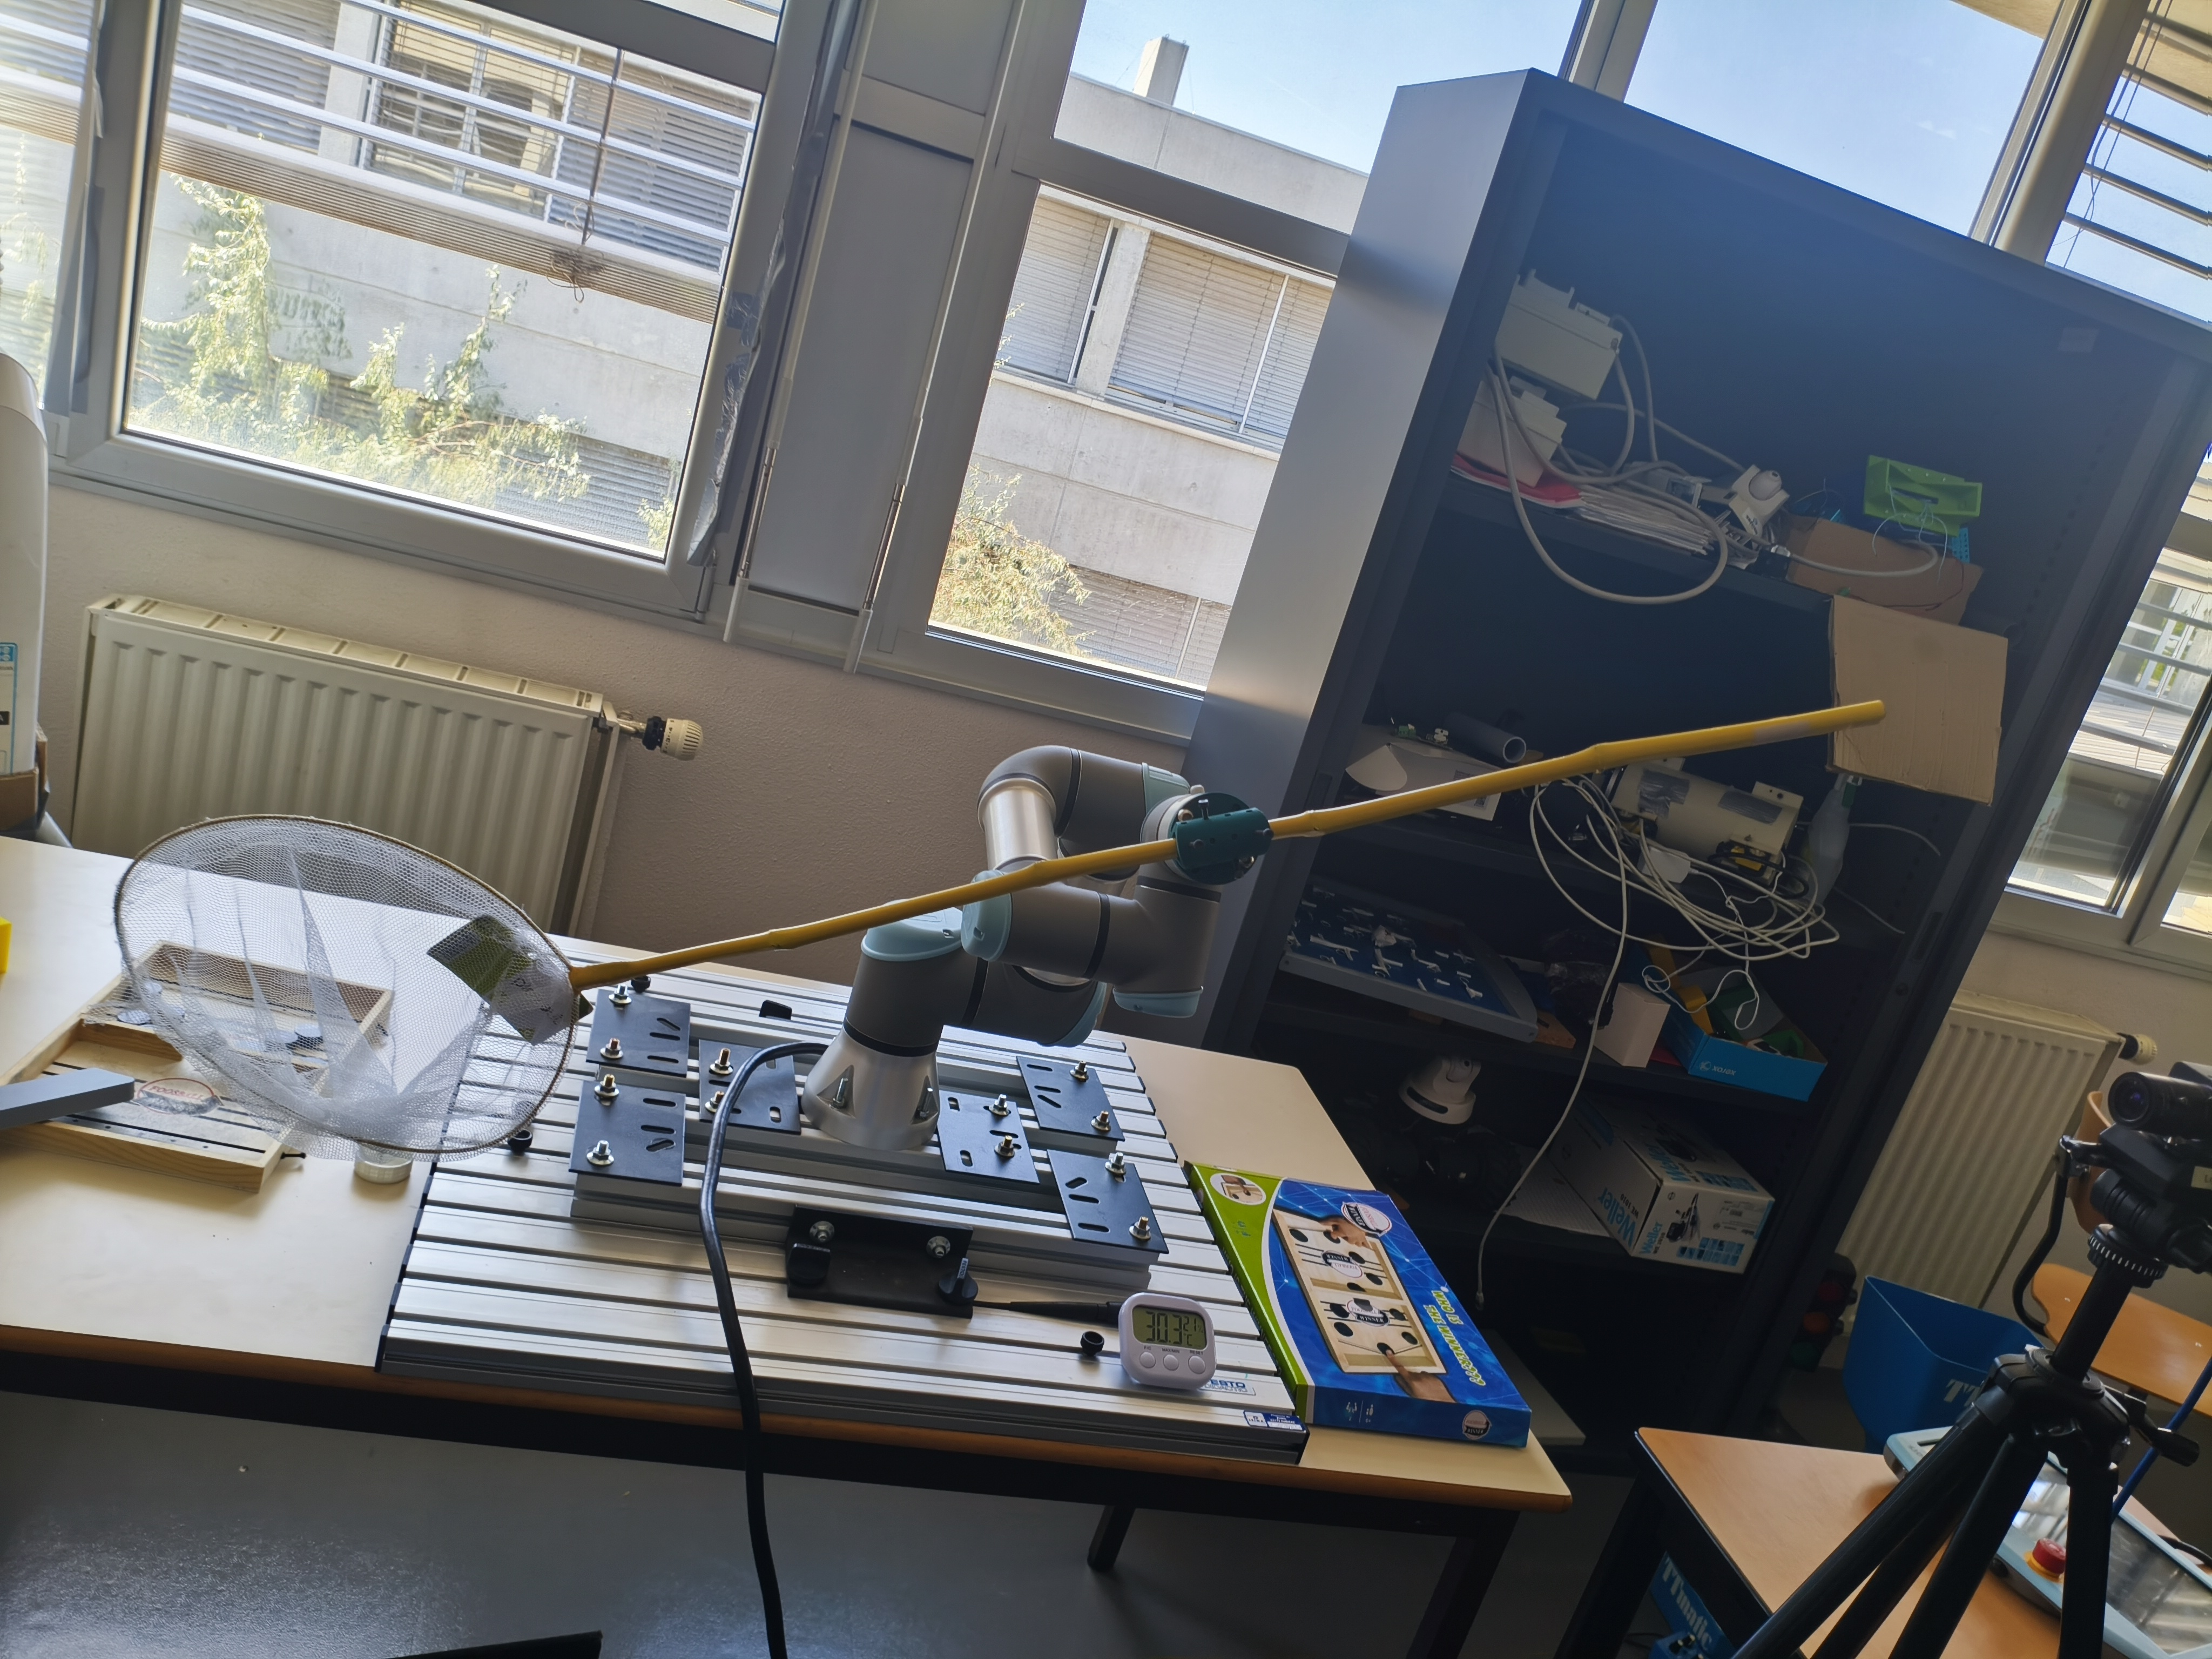
\includegraphics[width=0.72\textwidth]{images/Support_Filet.jpg}
  \caption{Filet d'interception monté sur le UR3e par le support imprimé en 3D, dans la configuration des essais réels.}
  \label{fig:support-filet-ensemble}
\end{figure}

La pièce se monte sur le poignet du robot et reçoit le manche du filet dans un logement traversant. Le maintien est assuré par des vis de pression qui viennent serrer directement le manche. Comme un filetage imprimé résisterait mal au serrage répété, des écrous sont noyés dans la pièce pendant l'impression et font office de filetage, les vis prenant dans un pas métallique, ce qui permet un serrage ferme sans dégrader le plastique. Le manche est ainsi maintenu perpendiculairement à l'axe du poignet, ce qui place le cercle du filet en porte-à-faux d'un côté de l'effecteur. C'est cette géométrie, et notamment le côté de montage, qui définit la position du centre du filet utilisée par la politique d'interception; elle correspond aux deux variantes gauche et droite évoquées dans le corps du rapport, une politique apprise pour un côté n'étant pas transférable à l'autre.

Le compromis principal de conception est la masse et le bras de levier, car le filet doit rester assez rigide pour que la position de son centre reste prévisible pendant les mouvements rapides du robot, tout en ajoutant le moins d'inertie possible en bout de bras.

\begin{figure}[H]
  \centering
  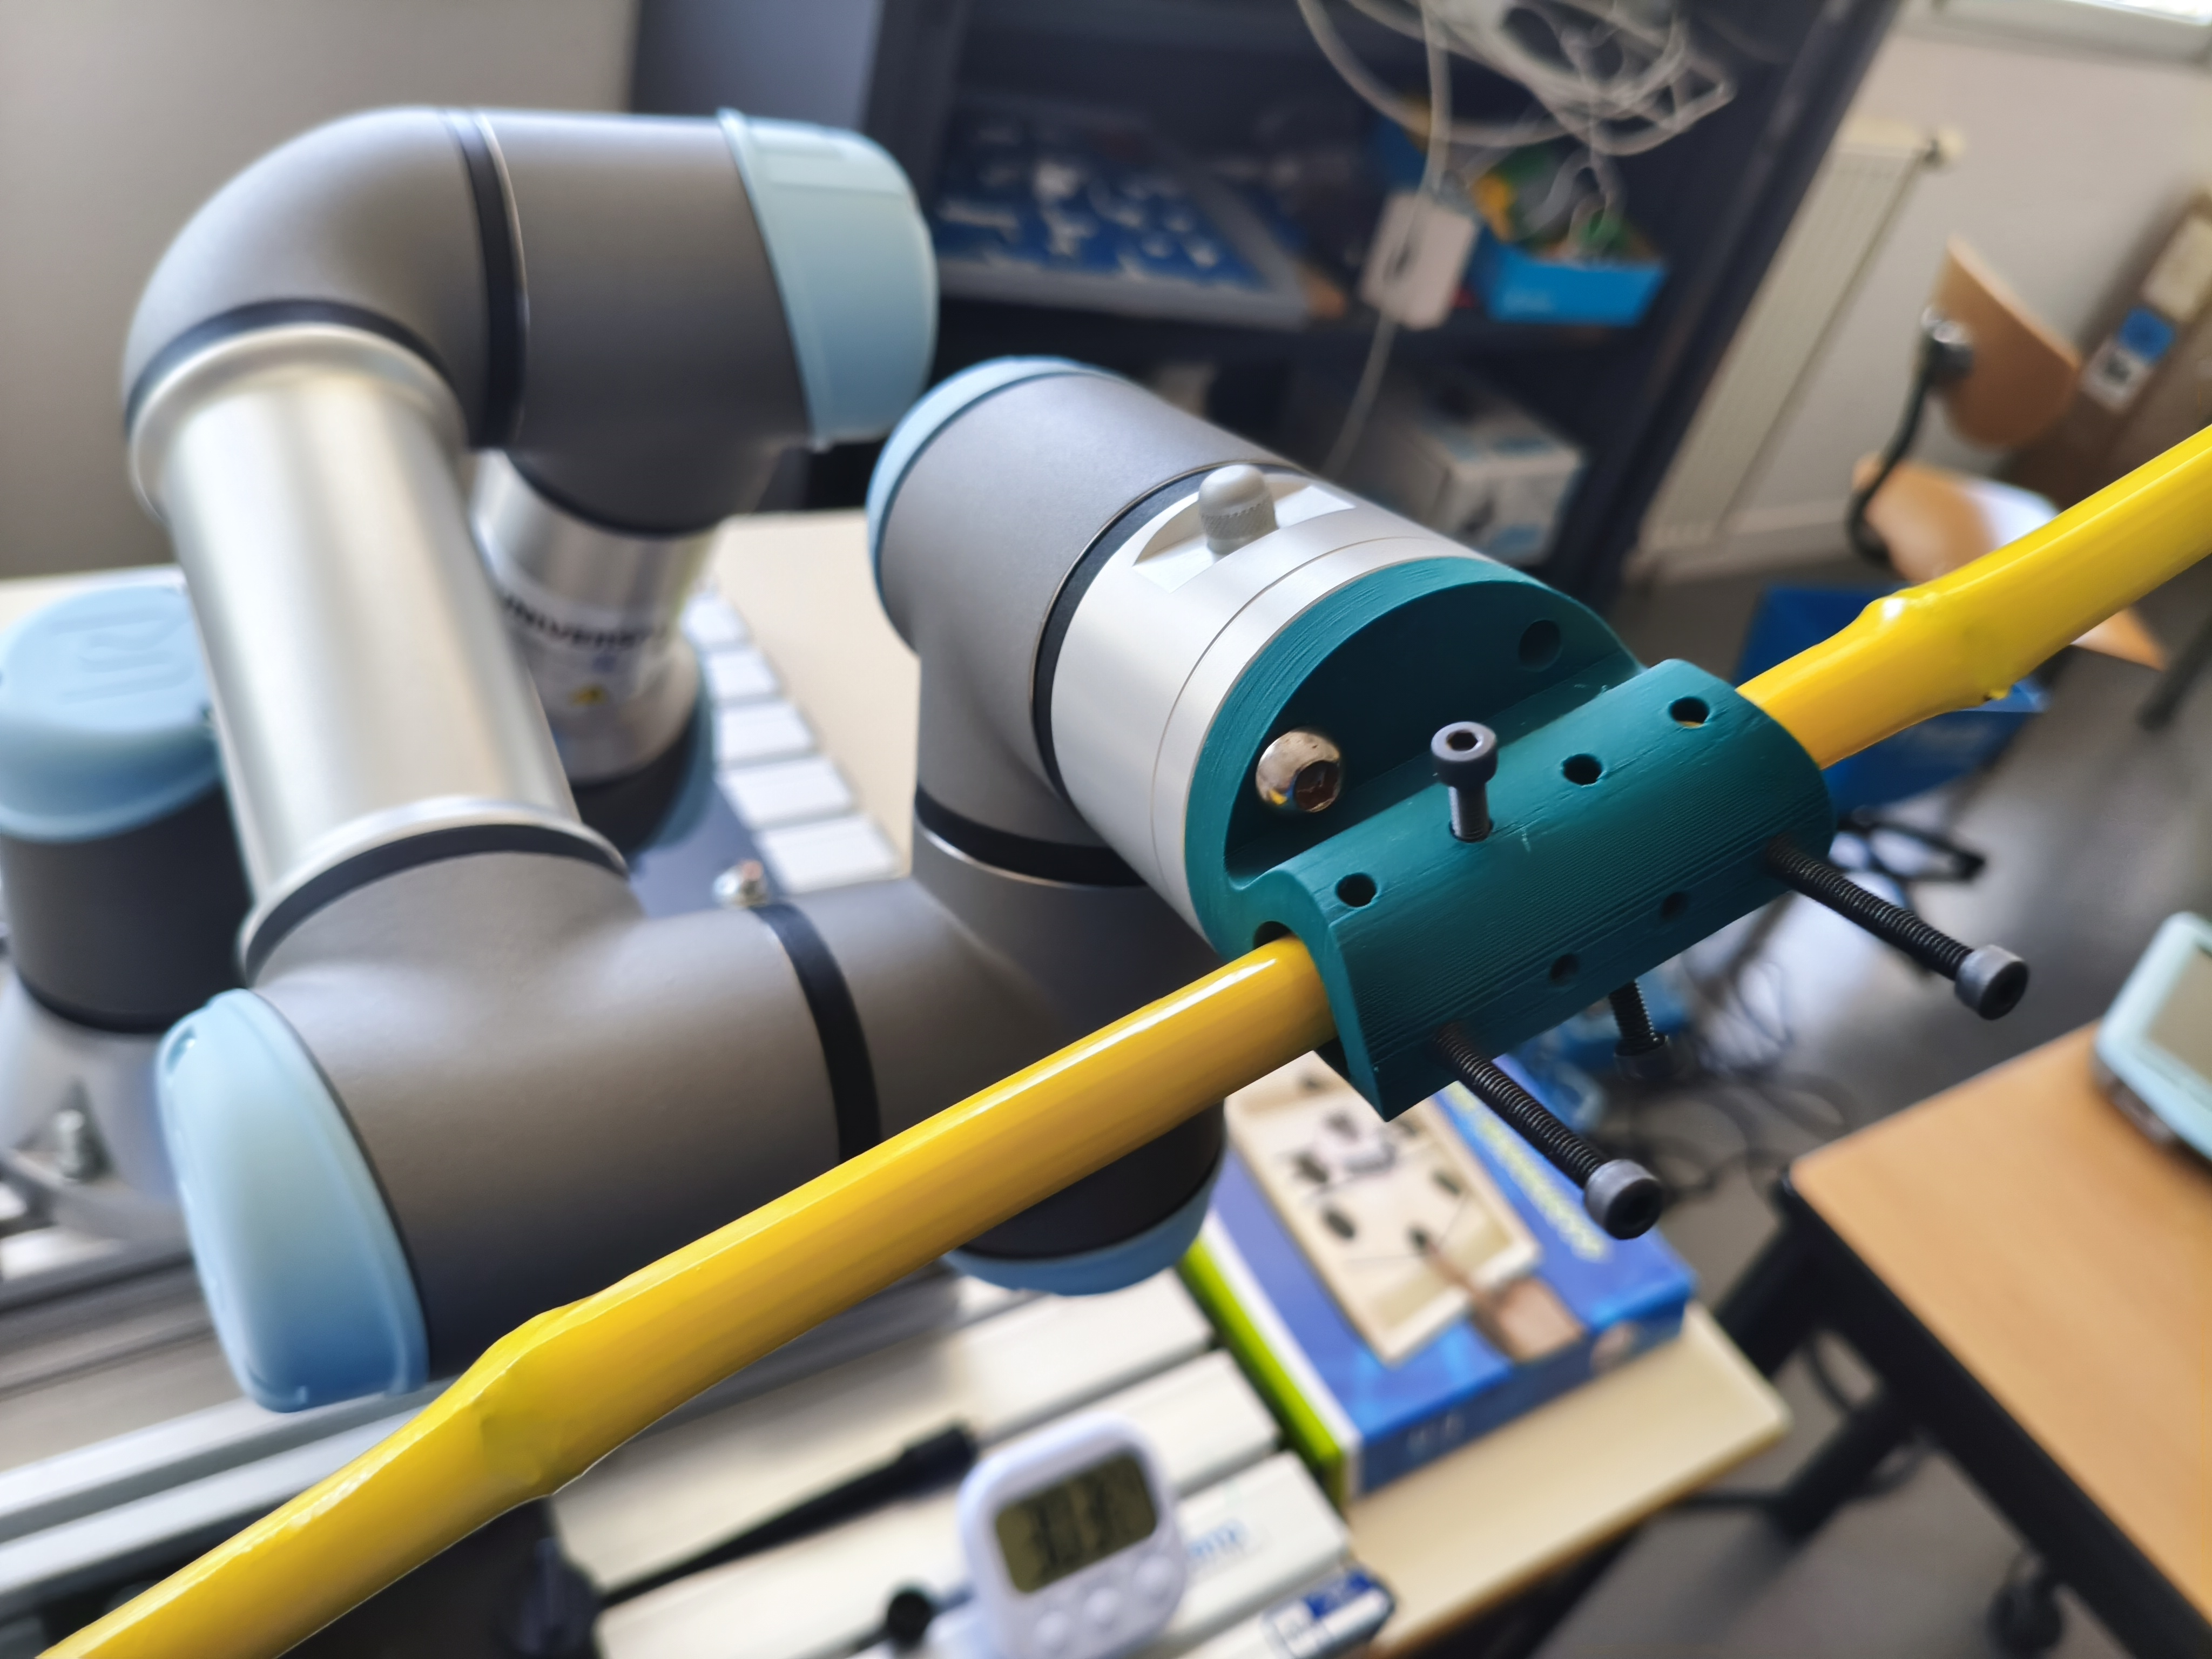
\includegraphics[width=0.72\textwidth]{images/Support_filet_Zoom.jpg}
  \caption{Détail de la fixation: le manche du filet traverse la pièce imprimée et est bloqué par des vis de pression, qui prennent dans des écrous noyés dans l'impression.}
  \label{fig:support-filet-zoom}
\end{figure}

\clearpage
\phantomsection
\addcontentsline{toc}{chapter}{Bibliographie et webographie}
\begin{thebibliography}{99}

\bibitem{antonio-stage}
Antonio Claudio De Sousa Dos Santos Filho,
\emph{Computer Vision, Reinforcement Learning and Skill Transfer in Robotic: Application to a Dynamic Task}, rapport de stage, document fourni.

\bibitem{cir-itps}
CAP 20-25,
\emph{Le Centre International de Recherche ``Innovative Transportation and Production Systems'' - CIR ITPS}.
\url{https://cap2025.fr/fr/challenge2}

\bibitem{cir-itps-useful}
CAP 20-25,
\emph{Useful information of CIR ITPS}.
\href{https://cap2025.fr/en/research/scientific-challenges/international-research-centre-on-innovative-transportation-and-production-systems/useful-information-of-cir-itps}{https://cap2025.fr/.../useful-information-of-cir-itps}

\bibitem{uca-universite}
Université Clermont Auvergne,
\emph{Site institutionnel de l'Université Clermont Auvergne}.
\url{https://www.uca.fr/}

\bibitem{institut-pascal}
Institut Pascal,
\emph{Présentation de l'Institut Pascal}, site officiel.
\url{http://www.institutpascal.uca.fr/index.php/fr/l-institut-pascal/presentation}

\bibitem{ispr-axe}
Institut Pascal,
\emph{Axe Image, Systèmes de Perception, Robotique (ISPR)}, site officiel.
\url{http://www.institutpascal.uca.fr/index.php/fr/presentation-ispr}

\bibitem{ip-maccs}
Institut Pascal,
\emph{Équipe MACCS -- Modélisation, Autonomie et Contrôle dans les Systèmes Complexes}, site officiel.
\url{http://www.institutpascal.uca.fr/index.php/fr/maccs}

\bibitem{ip-comsee}
Institut Pascal,
\emph{Équipe ComSee -- Computers that See}, site officiel.
\url{http://www.institutpascal.uca.fr/index.php/fr/comsee}

\bibitem{inivation-dvxplorer}
iniVation,
\emph{DVXplorer -- Hardware documentation}, documentation officielle.
\url{https://docs.inivation.com/hardware/current-products/dvxplorer.html}

\bibitem{inivation-docs}
iniVation,
\emph{Documentation officielle iniVation}.
\url{https://docs.inivation.com/}

\bibitem{lichtsteiner-dvs}
Lichtsteiner, P., Posch, C. et Delbruck, T.,
\emph{A 128$\times$128 120\,dB 15\,$\mu$s Latency Asynchronous Temporal Contrast Vision Sensor},
IEEE Journal of Solid-State Circuits, vol. 43, n\textsuperscript{o} 2, p. 566--576, 2008.

\bibitem{gallego-survey}
Gallego, G., Delbrück, T., Orchard, G., Bartolozzi, C., Taba, B., Censi, A., Leutenegger, S., Davison, A. J., Conradt, J., Daniilidis, K. et Scaramuzza, D.,
\emph{Event-based Vision: A Survey},
IEEE Transactions on Pattern Analysis and Machine Intelligence, vol. 44, n\textsuperscript{o} 1, p. 154--180, 2022.

\bibitem{delbruck-goalie}
Delbruck, T. et Lang, M.,
\emph{Robotic Goalie with 3\,ms Reaction Time at 4\,\% CPU Load Using Event-Based Dynamic Vision Sensor},
Frontiers in Neuroscience, vol. 7, 2013.

\bibitem{falanga-avoidance}
Falanga, D., Kleber, K. et Scaramuzza, D.,
\emph{Dynamic Obstacle Avoidance for Quadrotors with Event Cameras},
Science Robotics, vol. 5, n\textsuperscript{o} 40, 2020.

\bibitem{glover-ball}
Glover, A. et Bartolozzi, C.,
\emph{Event-driven Ball Detection and Gaze Fixation in Clutter},
IEEE/RSJ International Conference on Intelligent Robots and Systems (IROS), 2016.

\bibitem{glover-tracking}
Glover, A. et Bartolozzi, C.,
\emph{Robust Visual Tracking with a Freely-moving Event Camera},
IEEE/RSJ International Conference on Intelligent Robots and Systems (IROS), 2017.

\bibitem{monforte-prediction}
Monforte, M., Arriandiaga, A., Glover, A. et Bartolozzi, C.,
\emph{Exploiting Event Cameras for Spatio-Temporal Prediction of Fast-Changing Trajectories},
IEEE International Conference on Artificial Intelligence Circuits and Systems (AICAS), 2020.

\bibitem{muglikar-calibration}
Muglikar, M., Gehrig, M., Gehrig, D. et Scaramuzza, D.,
\emph{How to Calibrate Your Event Camera},
IEEE/CVF Conference on Computer Vision and Pattern Recognition Workshops (CVPRW), 2021.

\bibitem{ros2-docs}
Open Robotics,
\emph{ROS 2 Documentation}, documentation officielle.
\url{https://docs.ros.org/}

\bibitem{opencv-calib3d}
OpenCV,
\emph{Camera Calibration and 3D Reconstruction -- calib3d module}, documentation officielle.
\url{https://docs.opencv.org/4.x/d9/d0c/group__calib3d.html}

\bibitem{raylib}
raylib,
\emph{raylib -- A simple and easy-to-use library to enjoy videogames programming}, site officiel.
\url{https://www.raylib.com/}

\bibitem{nvidia-isaac-sim}
NVIDIA,
\emph{Isaac Sim -- Robotics Simulation and Synthetic Data Generation}, site officiel.
\url{https://developer.nvidia.com/isaac/sim}

\bibitem{nvidia-isaac-lab}
NVIDIA,
\emph{Isaac Lab -- Robot Learning Framework}, site officiel.
\url{https://developer.nvidia.com/isaac/lab}

\bibitem{v2e-github}
SensorsINI,
\emph{v2e: From video frames to DVS events}, dépôt GitHub.
\url{https://github.com/SensorsINI/v2e}

\bibitem{v2e-paper}
Hu, Y., Liu, S.-C. et Delbruck, T.,
\emph{v2e: From Video Frames to Realistic DVS Events}, CVPR Workshops, 2021.
\url{https://openaccess.thecvf.com/content/CVPR2021W/EventVision/html/Hu_v2e_From_Video_Frames_to_Realistic_DVS_Events_CVPRW_2021_paper.html}

\bibitem{schulman-ppo}
Schulman, J., Wolski, F., Dhariwal, P., Radford, A. et Klimov, O.,
\emph{Proximal Policy Optimization Algorithms}, arXiv, 2017.
\url{https://arxiv.org/abs/1707.06347}

\bibitem{repo-stage}
Ajvazi, R.,
\emph{Perception événementielle, calibration et interception temps réel: chaîne C++/ROS 2 du stage}, dépôt de code.
\url{https://github.com/RigonAj/Stage}

\bibitem{repo-isaac}
Ajvazi, R.,
\emph{Environnement Isaac Lab et apprentissage PPO de l'interception avec un UR3e}, dépôt de code.
\url{https://github.com/RigonAj/6-Dof-Ur3e-Catch-a-ball}

\end{thebibliography}

\end{document}
